\chapter{激光单空泡在软、固界面附近的脉动}


空泡在不同边界条件下的脉动是一个常作常新的研究课题。本章主要针对空泡处于不同环境中的脉动进行仿真计算。其中液体环境大致分为水与软物质相接触和与固体物质相接触的状态。而水与软物质也可大概区分为液-气、液-液两种条件。在探讨空泡在这些界面附近的脉动时,我们忽略现实中存在的多种界面形状,而只分析平面的界面。

 \section{单空泡在自由域内的脉动}
%通过前述模型计算获得的能量沉积型空泡在自由域内脉动的半径-时间曲线与 Keller-Miksis 模型的对比如图所示。
通过前文\ref{chap2.5}中设计的算法,数值模拟获得能量沉积型空泡在自由域内的脉动。结果如图\ref{fig3.single}所示。
\begin{figure}[h]
    \centering
    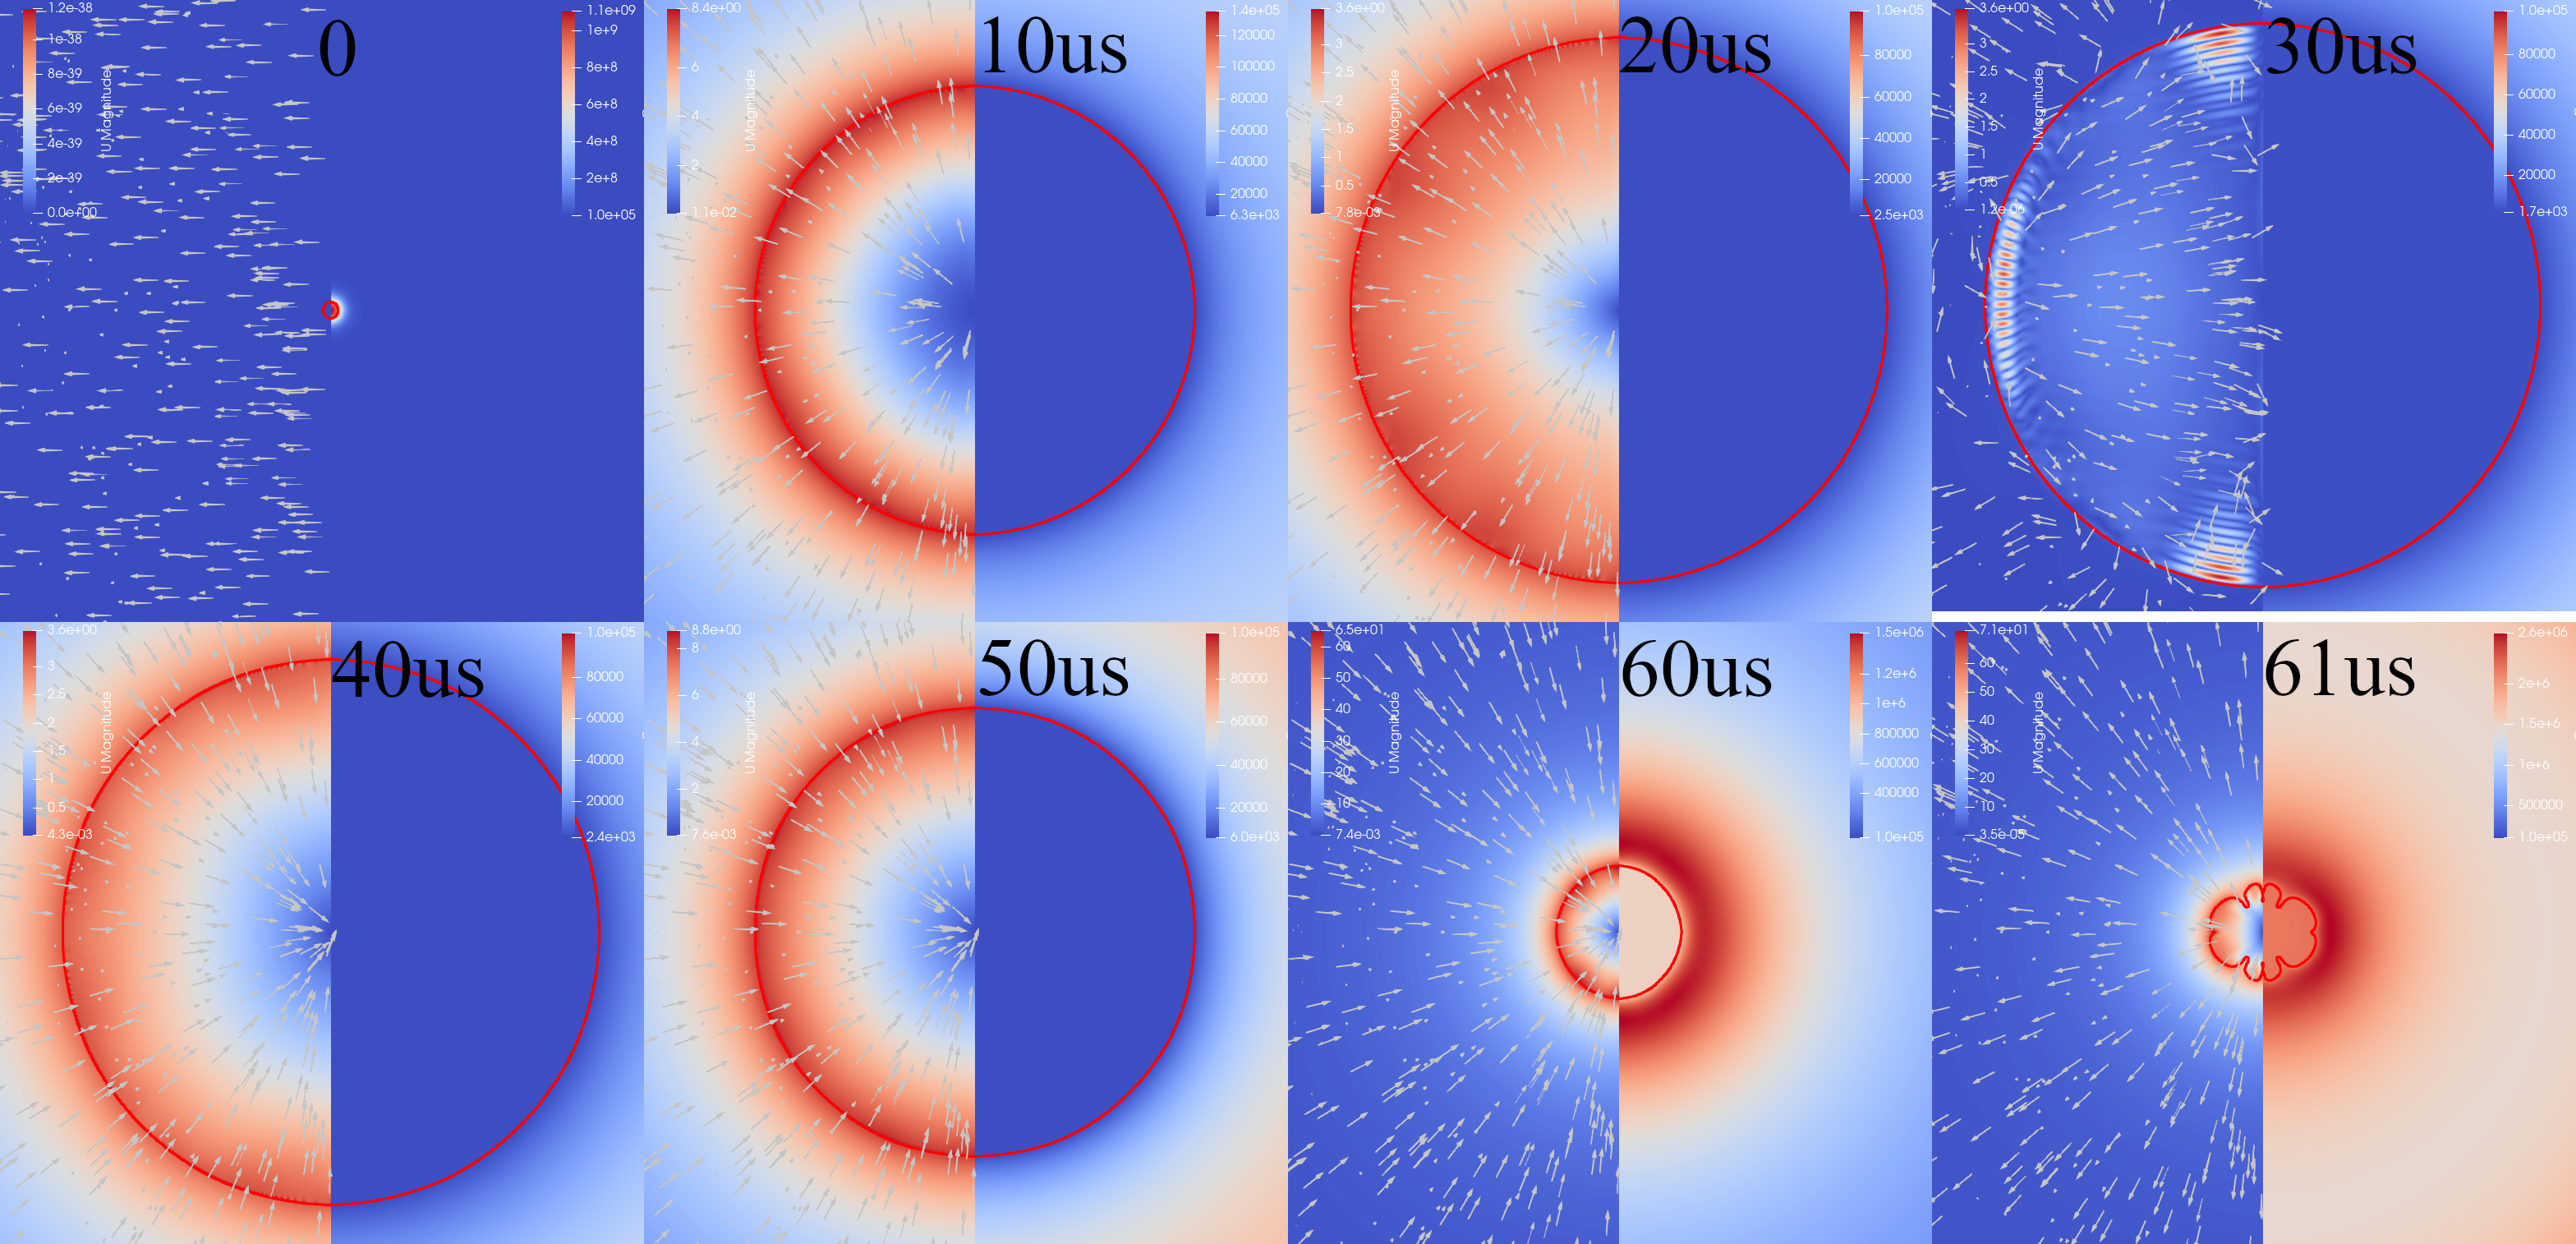
\includegraphics[width=0.9\linewidth]{img/fig3.single.png}
    \caption[自由域内单空泡的相-压力-速度云图]{自由域内单空泡的相-压力-速度云图,空泡壁面用红色线标识,每一帧的右侧是压力场云图,左侧是速度场云图,用颜色表示速度值,用箭头表示速度的方向。}
    \label{fig3.single}
\end{figure}

图\ref{fig3.single}中,空泡经历了一个完整的生命周期,从初始状态,然后随之高速膨胀,和减速膨胀,到最大泡半径。随后开始缓慢收缩,随着周围水的运动加速,收缩加剧,在$60\mu s $左右收缩到最小状态,水体相互碰撞,辐射一个冲击波,最后开始再次膨胀。

此例的计算主要为模拟空泡在自由域中的脉动,获得自由域中的体积等效半径,以为下文中空泡半径对比的基准。算法的有效性经过前文验证。同时应该注意,自由域的含义是一个简化的理想的环境,其不考虑重力和边界等问题。这样的环境在物理现实中并不存在。


\section{单空泡在水与软物质界面附近的脉动}



本章中重新定义了异于上一章但通行于学界的用于量化单空泡与界面距离的无量纲距离参数 $\gamma$:
$$\gamma=\frac {D} {R_\mathrm{0}}
$$
此处 $D$ 代表了空泡初生位置距离界面的距离,$R_\mathrm{0}$ 代表了空泡在自由域内脉动时的最大泡半径。
针对界面两边不同的物质,定义了水、气、和硅油($\mathrm{C_2H_6OSi}$),其性质如表\ref{tab:3.1}所示。

\begin{table}[h]
    \centering
    \begin{tabular}{|c|c|c|c|}
    \hline
    \textbf{液体参量} &  \textbf{水} &  \textbf{气} &  \textbf{硅油($\mathrm{C_2H_6OSi}$)}   \\  \hline
    \textbf{B} & 3.036e8&0 &1.5e8 \\  \hline
    \textbf{$\rho_0$} & 998.2061&0.12 &960 \\  \hline
    \textbf{$p_0$} &  101325&10320 &101325 \\  \hline
    \textbf{$\gamma$} &  7.15&1.33 &604 \\  \hline
    \textbf{$Cp$} & 4195 & 1007&2240 \\  \hline
    \textbf{$Hf$} &  0&0 &0 \\  \hline
    \textbf{$\mu$} & 1e-3& 1.84e-5&1e-1 \\  \hline
    \textbf{$Pr$} & 2.289& 0.7&6  \\  \hline

    \textbf{$\sigma_{air}$} & 0.0725& /&0.02  \\  \hline
        \textbf{$\sigma_{water}$} & /& 0.0725&0.03  \\  \hline
            \textbf{$\sigma_{oil}$} & 0.03& 0.02&  / \\  \hline
    
    \end{tabular}
    \caption[水,气,硅油($\mathrm{C_2H_6OSi}$)的液体参量]{水,气,硅油($\mathrm{C_2H_6OSi}$)的液体参量,另附表面张力系数于下。}
    \label{tab:3.1}
\end{table}

\begin{figure}[h]
    \centering
    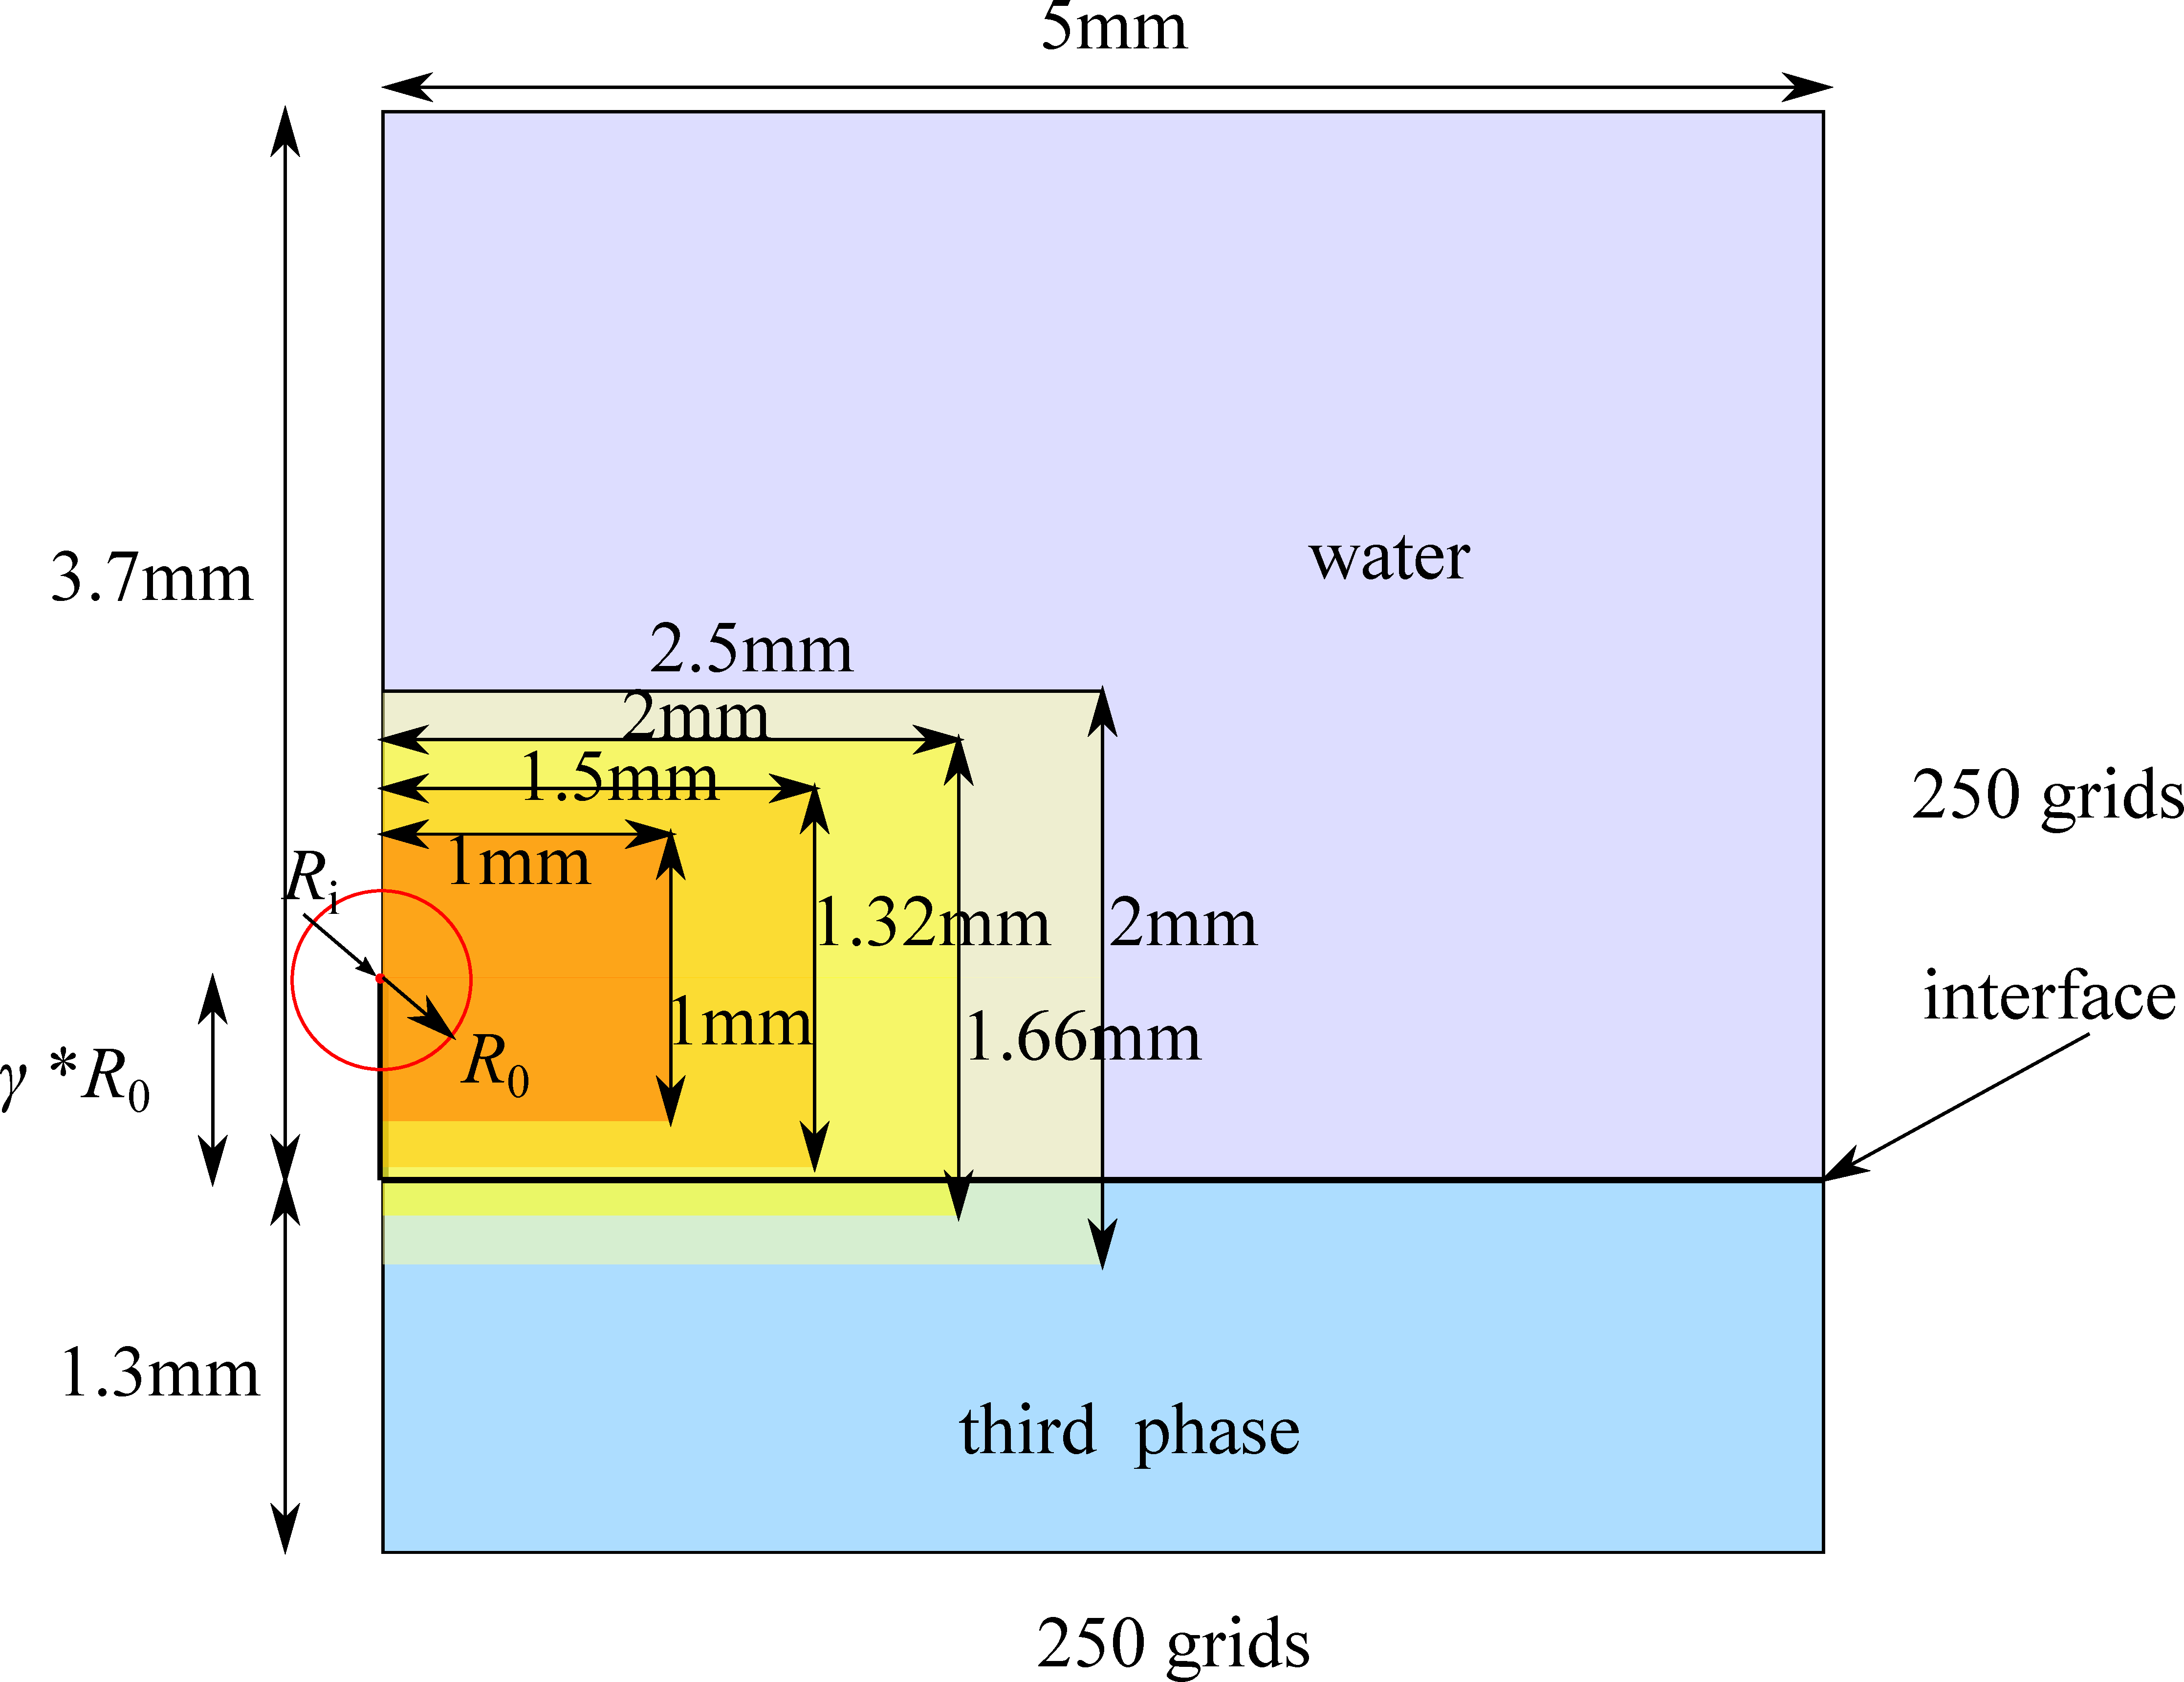
\includegraphics[width=0.7\linewidth]{img/interface.pdf}
    \caption{激光致空泡在软物质界面附近的脉动计算域设置}
    \label{fig:interface}
\end{figure}

软物质界面情景除了物性,使用相同的计算域和计算设置。除了对称轴使用对称边界,旋转面使用wedge边界,其他边界都是“wavetransform”的无反射压力边界,和速度“pressureInletOutletVelocity” 流入流出边界。初始的网格密度为$250\div5mm=50/mm$。经过四次加密,每次加密在选定区域内的$X,Y$方向上数量加倍,也就是区域内一个网格变四个网格。在能够覆盖空泡最大泡半径的区域内,网格密度达到了$800/mm$。不同$\gamma$下的计算域由图\ref{fig:interface}给出。其中空泡的初始半径和最大泡半径使用(12.5$\mu$m-320$\mu$m)这一组合。初始空泡时,半径用10个网格解析。全流场计算域网格数917200。图中的第三相在水气界面案例中为与空泡同物性的气,在水油界面中为硅油。共计算了$\gamma\in \left[0.1:0.1:2\right]$共20组案例。


\subsection{单空泡在水气界面附近的脉动}



\begin{figure}[h]
    \centering
    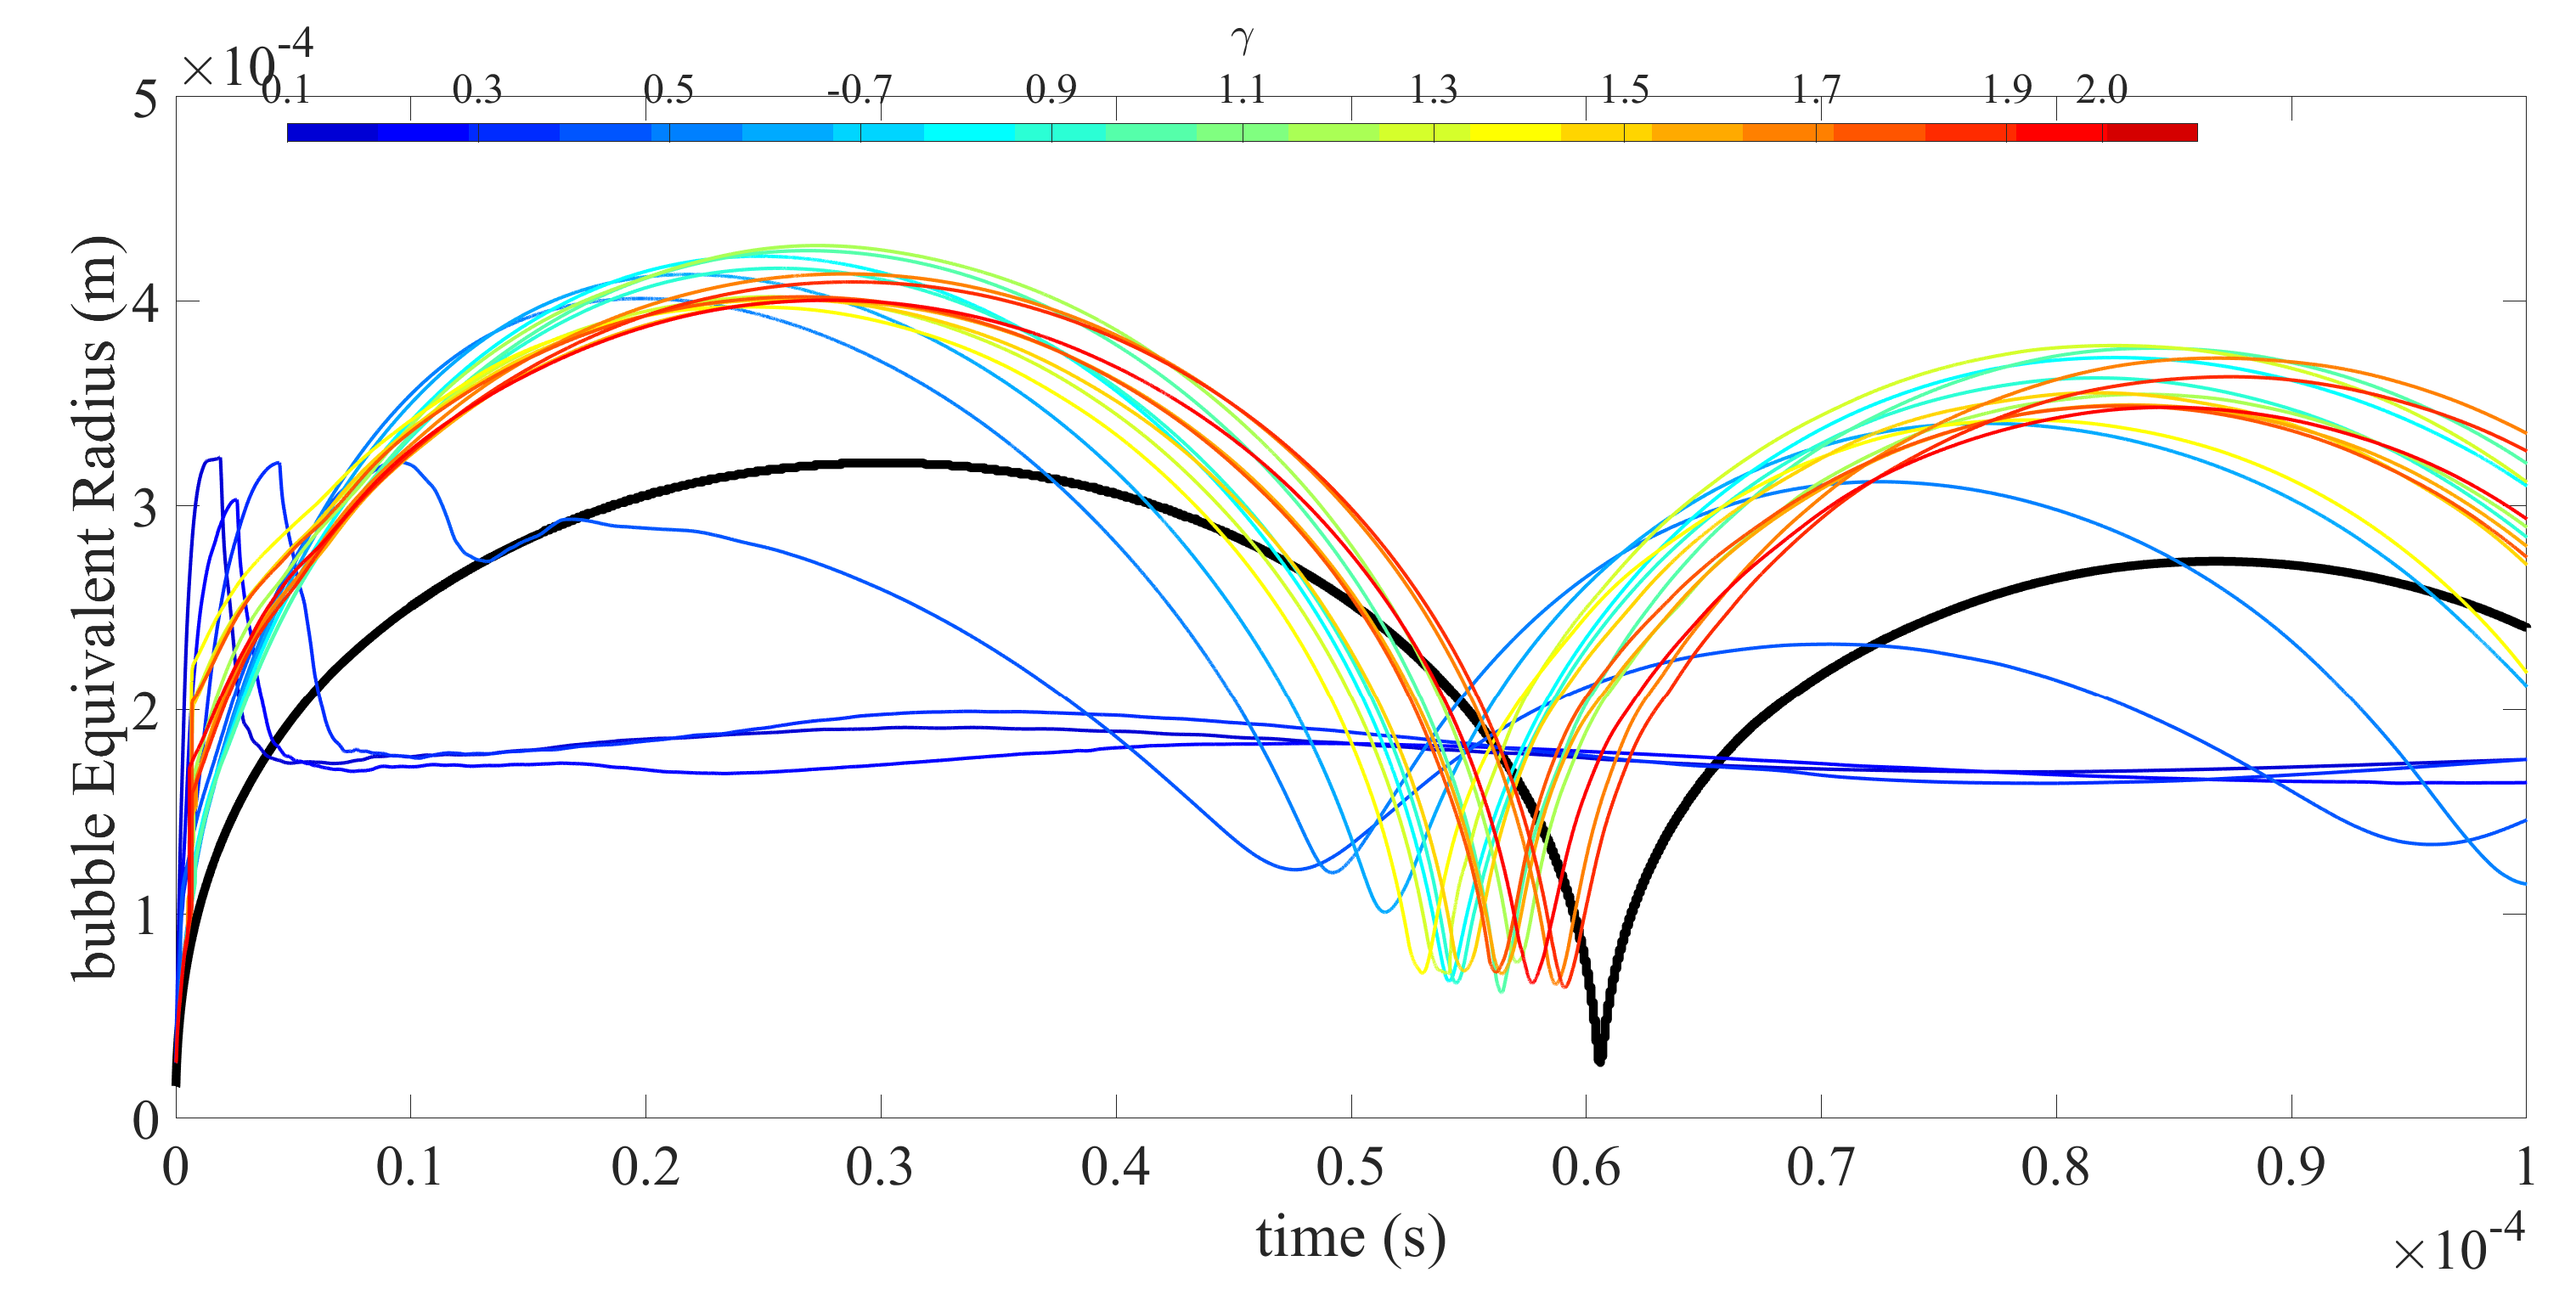
\includegraphics[width=0.9\linewidth]{img/fig3.airradius.eps}
    \caption[空泡距水气界面不同相对距离情形下的泡半径对比图]{空泡距水气界面不同相对距离情形下的泡半径对比图。图中黑色实线为自由域中的模拟结果。}
    \label{fig3.airradius}
\end{figure}

空泡在水气界面附近脉动时,会形成独特的动力学特征,比如双向的射流和王冠形喷溅等。本节中,忽略重力的作用,仅从压强、惯性、张力、粘性和密度等角度考虑空泡在水气界面附近的运动。

图\ref{fig3.airradius}是20组空泡距水气界面不同相对距离情形下的泡半径对比图。图中数据通过模拟计算中每一步记录的空泡体积获得。即$R=\sqrt[3]{\frac{3((360/\alpha)V)}{4\pi}}$。$\alpha$是计算域的张角,前文中有述。
首先发现,空泡在水气界面附近的情况下,最大泡半径获得了提升,而生存周期则获得减小。这是因为在水气界面附近时,空泡推动低密度,低粘的气体相比水更加容易,也就使得惯性驱动的空泡膨胀能够获得更大的半径。

同时可以看到在$\gamma\leq0.3$时,空泡体积等效半径形成的曲线会出小一个暴增,然后急剧减小,随后保持稳定的过程。这是因为空泡距离界面过近形成爆破(burst)效果。爆破指空泡的气体在膨胀过程中,冲破液体表面的阻隔,直接与液面外的气体相联通。在这几个案例中,空泡的气体释放到外界气体中。但因为在模型计算中,将界面气体处理成具有气体物性的第三相,故而仍能追踪其逸出部分在101325Pa下的体积。在其他情景下,空泡半径随$\gamma$增长而减小,其生存周期也逐渐趋同于自由域空泡。

综合考量这20组模拟结果,粗略的将其分为三种情况:A.爆破式($\gamma\leq 0.3$);B.皇冠射流式($0.4\leq\gamma\leq 1.4$);C.突起式$\gamma\geq 1.5$)。因忽略重力作用,实验的分界点与以上的三个值可能稍有不同。


\begin{figure}[h]
    \centering
    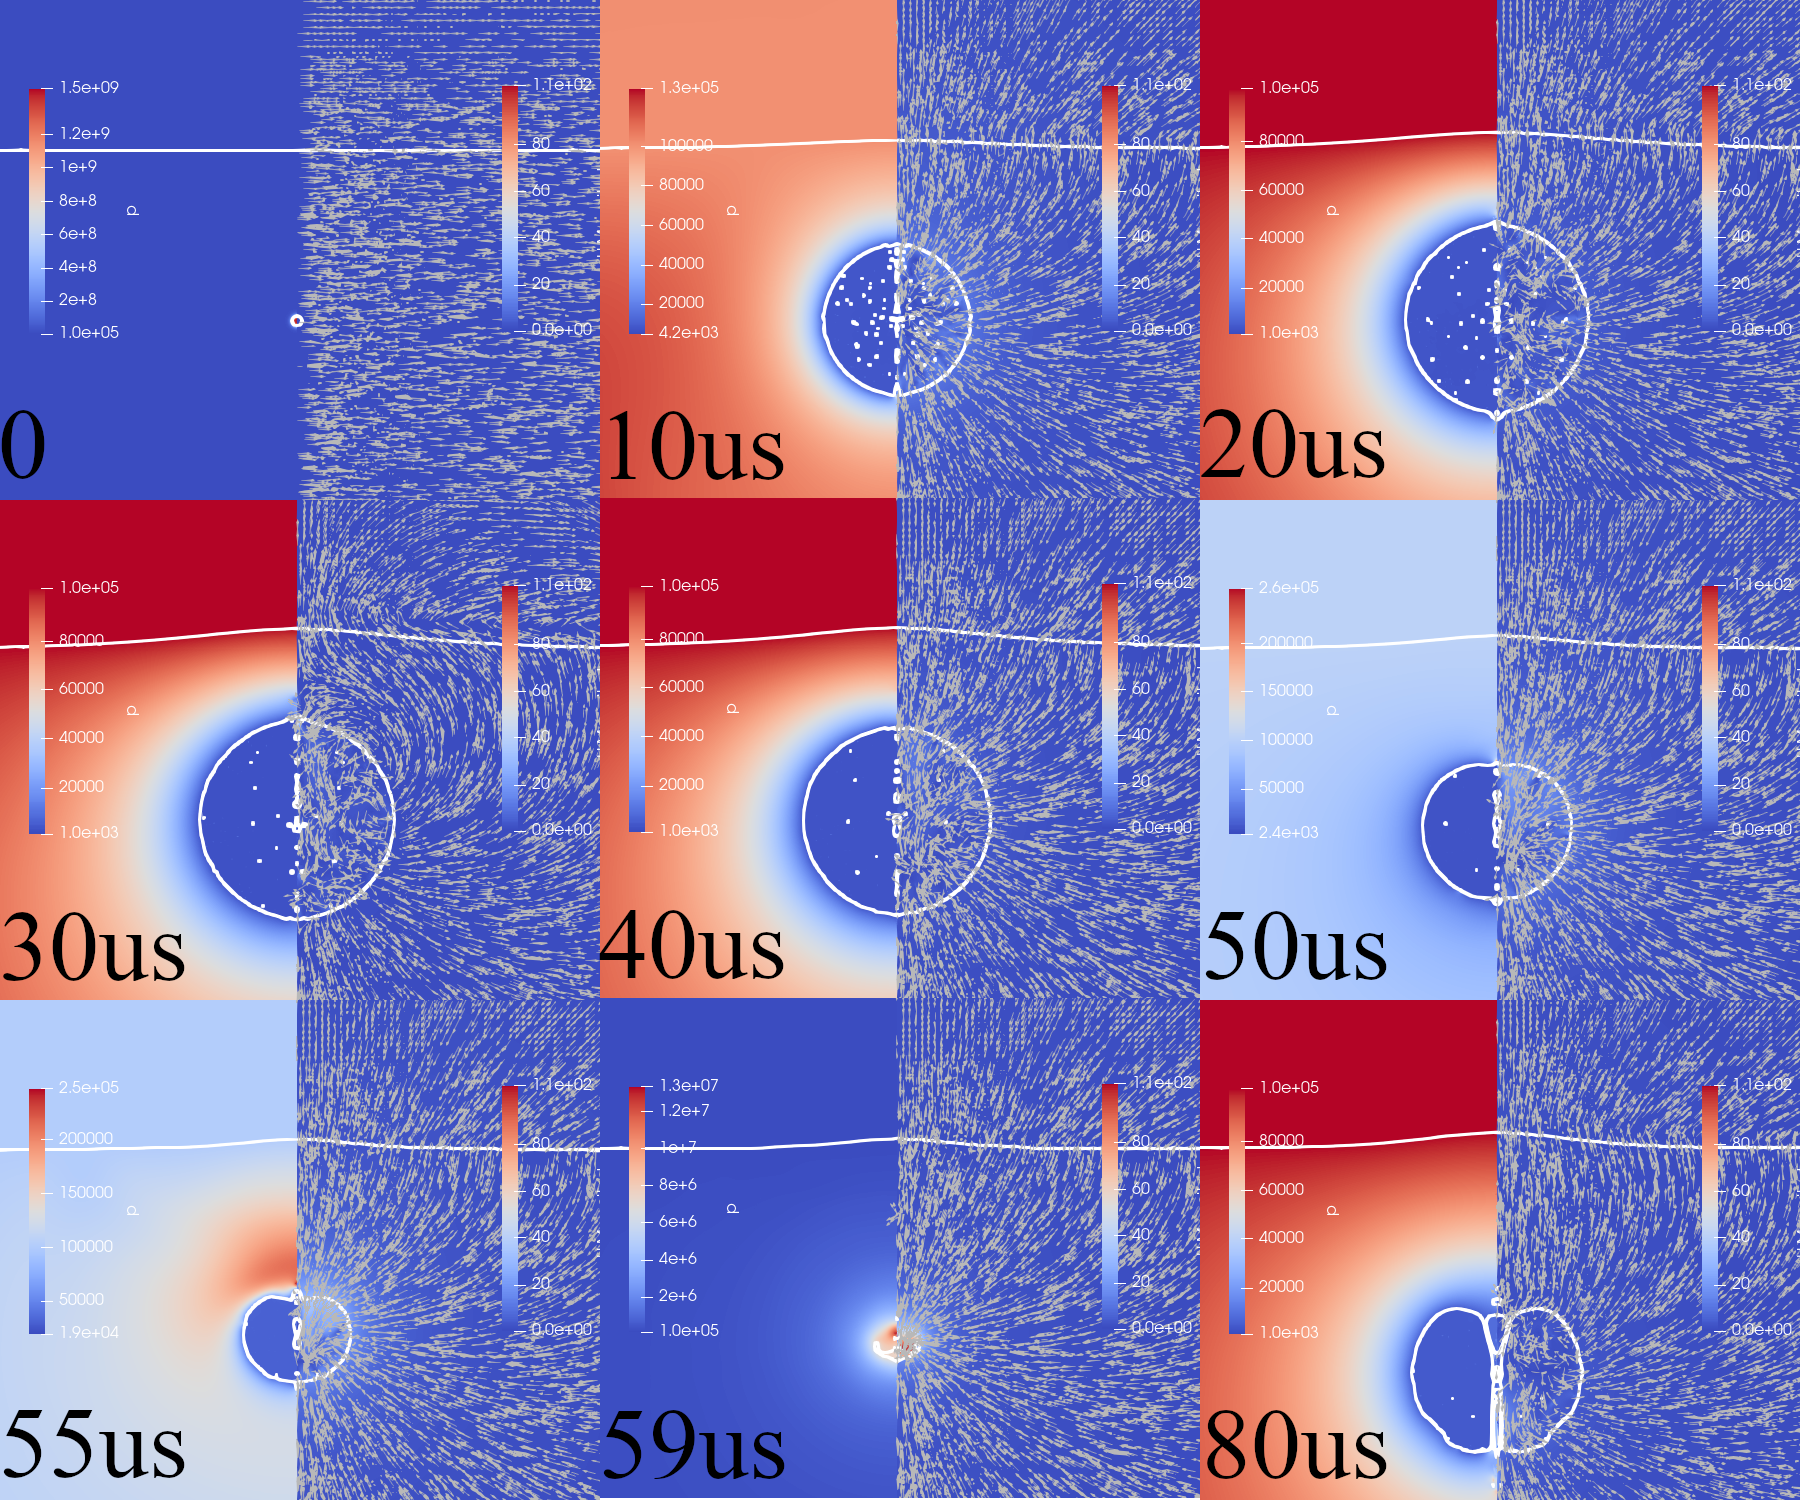
\includegraphics[width=0.9\linewidth]{img/fig3.air2.0.png}
    \caption[空泡距水气界面$\gamma=2.0$情形下的相-速度-压力云图]{空泡距水气界面$\gamma=2.0$情形下的相-速度-压力云图。图中白线代表水气界面。界面以上为气,界面以下为水。白线包裹的封闭联通域是空泡。每一帧的右侧是流域的速度场(单位m/s),左侧是压力场(单位Pa)。灰色箭头是速度场的方向。该帧的具体时刻标注在压力场的空白处。以下三个相-速度-压力云图按照同样的标注方式作图。}
    \label{fig3.air2.0pvp}
\end{figure}

图\ref{fig3.air2.0pvp}显示了空泡距水气界面$\gamma=2.0$情形下的相-速度-压力云图。其作为C.突起式$\gamma\geq 1.5$)空泡溃灭的一个典型案例。在这种情景下,空泡的射流情况可以用开尔文脉冲理论解释,即空泡形成远离界面的射流。同时,空泡的膨胀和收缩能够对水气界面形成改造。

第一栏的第一帧显示了该种情况下的计算初始情况,即一个存在于101325Pa的零速度域内的高压初始球形域。随后在第二帧($ 10\mu s$)中,空泡膨胀,在空泡内形成辐射状速度方向。但字啊空泡外的水中,在空泡下壁面,即南极附近,速度矢量仍呈辐射状。但在空泡下壁面以上的位置,水域的速度均最终指向自由界面。这是因为界面以上的气体的密度和粘度均小于水所形成的。值得注意的是,此时因空泡膨胀的推动,此时空泡正上方位置形成突起。第三帧($ 20\mu s$)中,空泡保持膨胀趋势。空泡内部的低压域自由液面以上的气体环境的101325Pa形成明显区别。

第二栏第一帧($ 30\mu s$)附近,空泡到达其最大泡半径,其空泡内部速度降到0,并丧失矢量方向。空泡外的上方形成自空泡始而指向空泡上方的气体区域。下一帧($ 40\mu s$)时,空泡的逐渐收缩。其主要受外界高压的驱动。在速度场中可以看到,与上两帧形成对比的是,速度方向形成了反转。这就在空泡外的上部形成速度自界面开始而指向空泡中心。在空泡外的下方,形成辐射状的指向空泡中心的收缩。在下一帧($ 50\mu s$)中,空泡继续收缩,同时空泡的上表面形成平化现象。相比横向的方向,指向空泡上方方向的速度矢量更多,同样也强于均匀的辐射收缩的下方。

在第三栏第一帧($ 55\mu s$)中,速度流延续了上文中的趋势,继续密集的指向了空泡上方位置。而因这种挤压在空泡的上方位置形成一个高压区域。这个高压区域将驱动空泡上方位置的水体继续加速的向空泡内部流动,即驱动形成射流,也成为支撑界面突起的一个因素。在下一帧($ 59\mu s$)中,自空泡上方射入的射流击穿空泡并撞击空泡下壁面。如此,形成撞击的高压。此时场内的速度仍如同上一帧一般的指向空泡的中心位置。在最后一帧($80 \mu s$)中,空泡中的击穿射流仍然存在,但同时空泡已经开始进入第二个生命周期。后续将在其新位置继续脉动。

本例中,空泡离界面位置较远,其形成的相互作用效果不明显。但其射流方向与使用开尔文脉理论(见章节\ref{chapter1.2.2.2})的参数$\bm\zeta=+0.195 \gamma^{-2} \bm n $计算获得的$\bm\zeta$预言的矢量方向和射流强度相一致。同时,自由界面并没有形成鲜明的变化,而只是因为空泡膨胀和空泡的不均匀收缩形成轻微的突起。

\vfill



\begin{figure}[h]
    \centering
    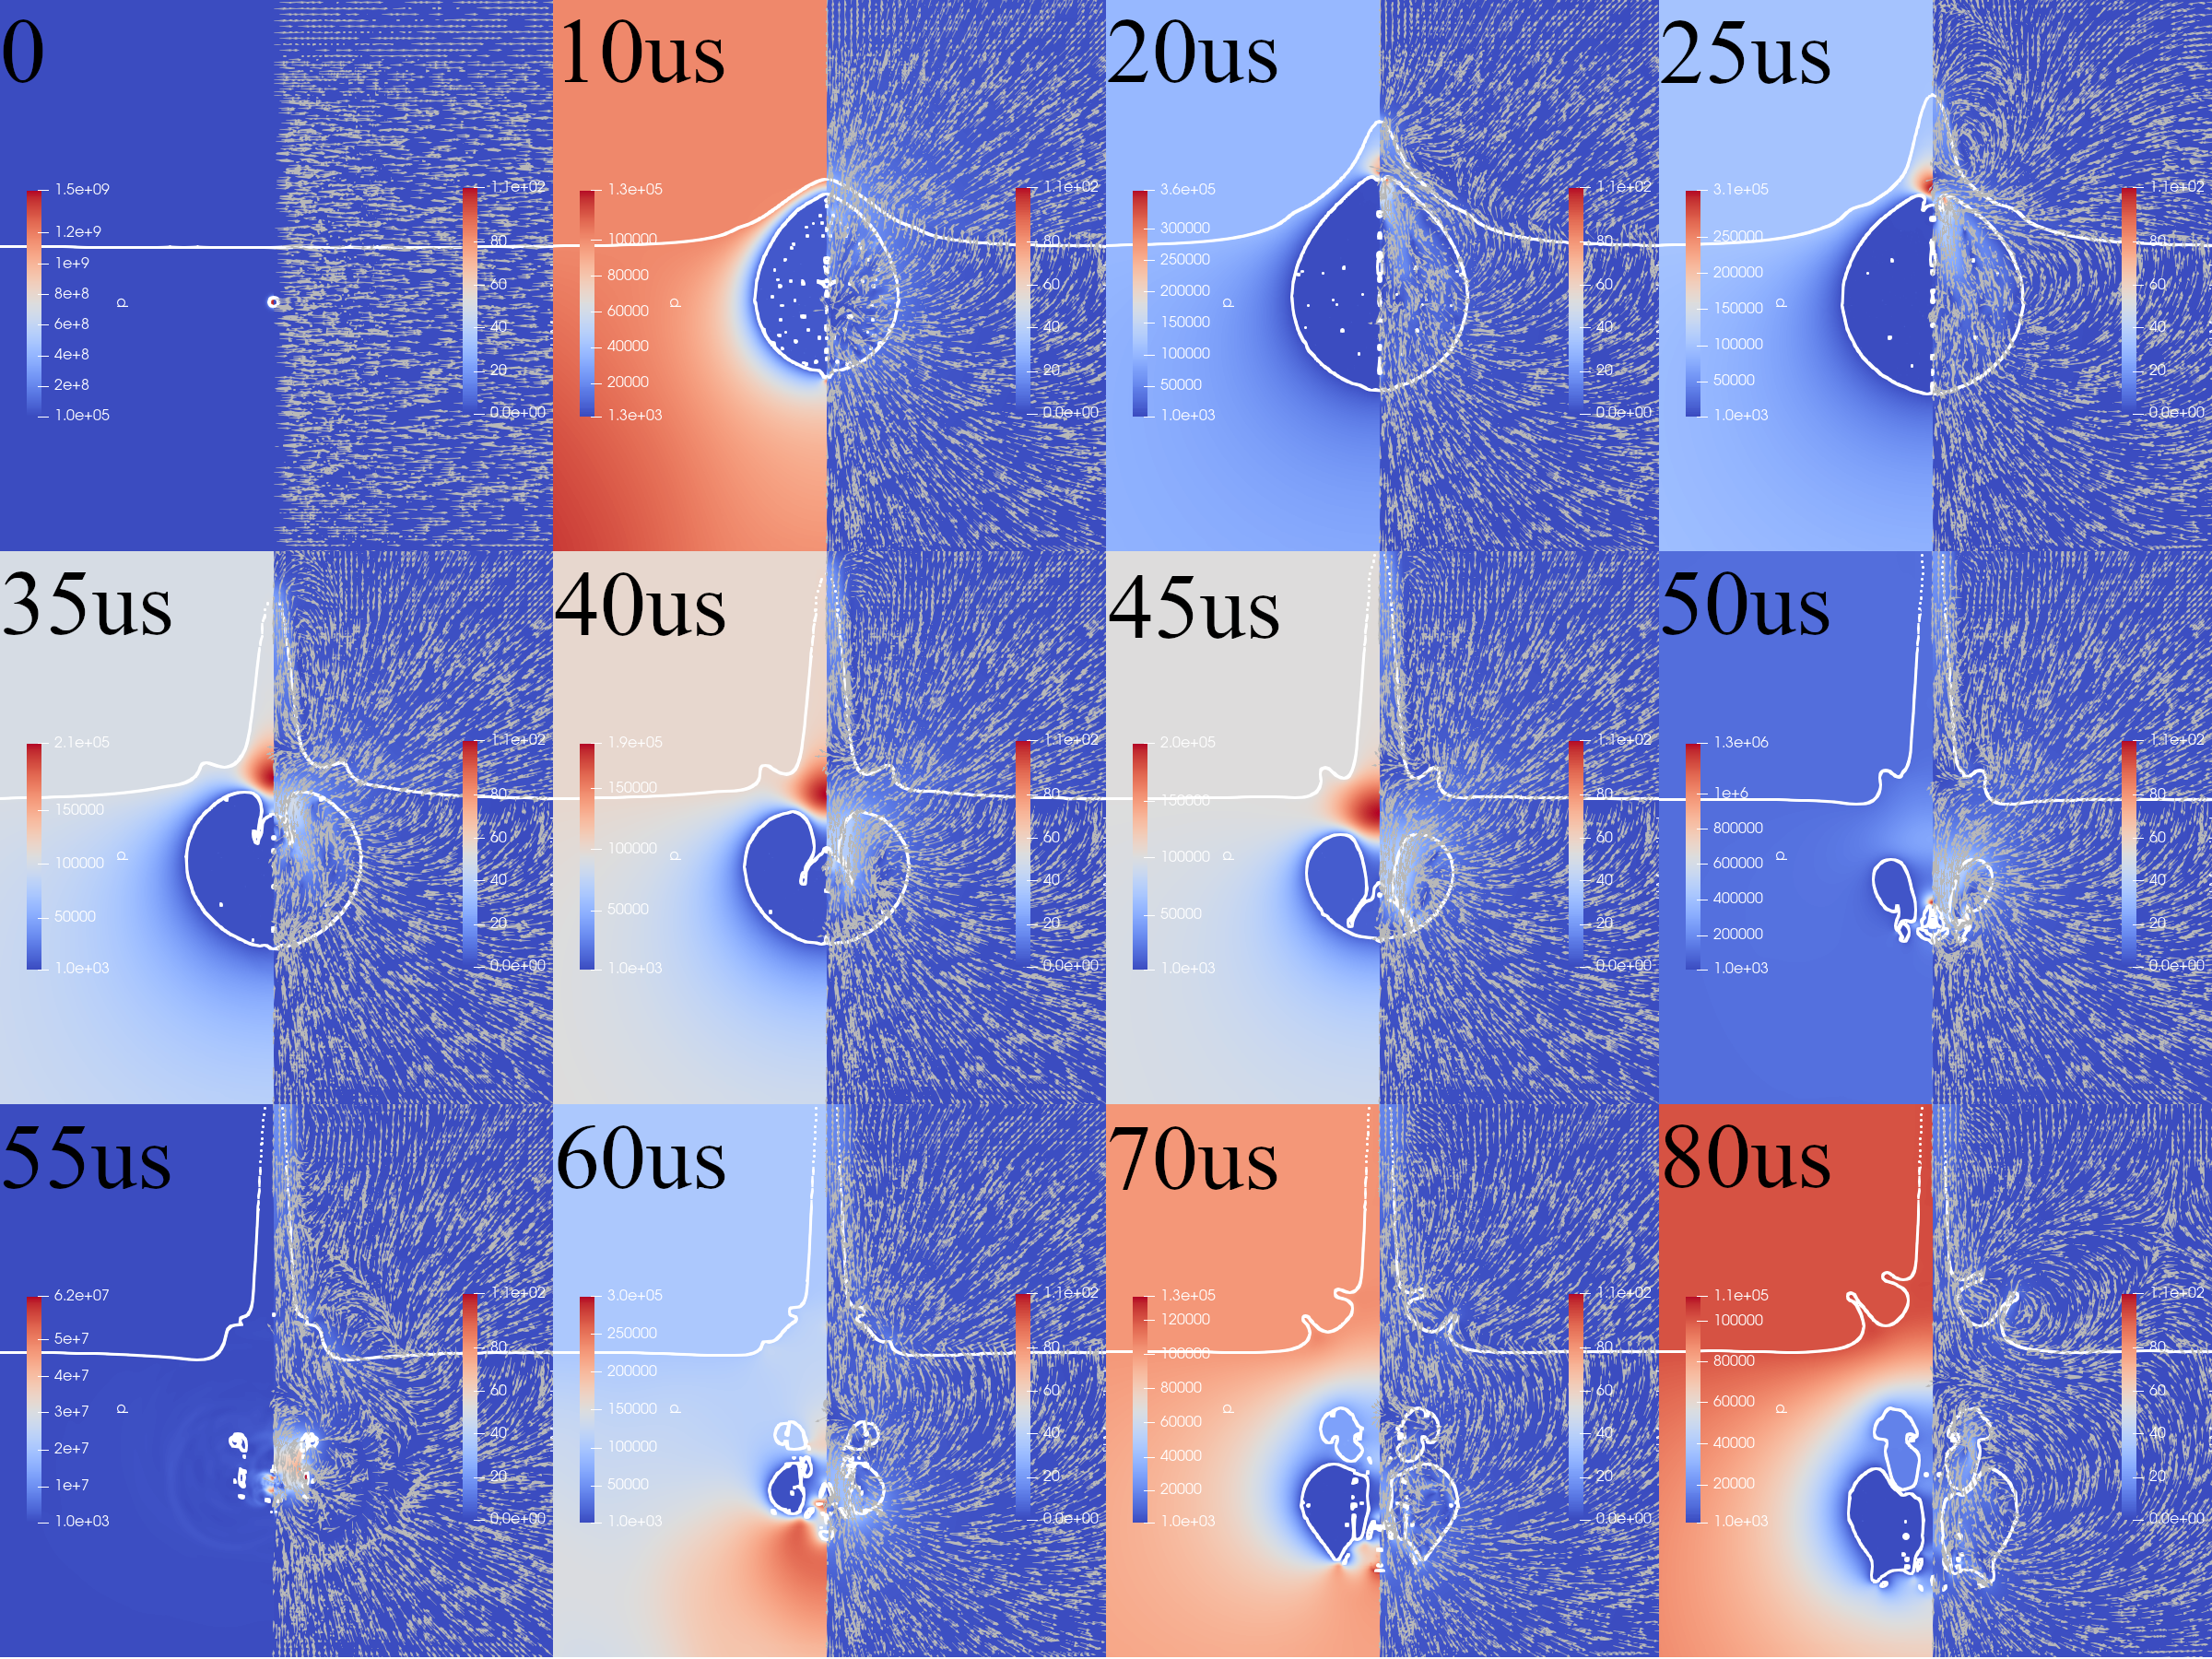
\includegraphics[width=0.9\linewidth]{img/fig3.air0.7.png}
    \caption{空泡距水气界面$\gamma=0.7$情形下的相-速度-压力云图}
    \label{fig3.air0.7pvp}
\end{figure}

图\ref{fig3.air0.7pvp}显示了空泡距水气界面$\gamma=0.7$情形下的相-速度-压力云图。该情景下形成了一种特殊的射流方式,即皇冠(crown)射流。其通常发生在空泡膨胀期,并形成于收缩过程中。本例作为B.皇冠射流式($0.4\leq\gamma\leq 1.4$)的一个典型案例解释该类型空泡脉动过程中的动力学现象。

在第一栏中,第一帧仍是空泡的初始状态。第二帧($10 \mu s$)中,空泡膨胀形成一个卵形壁面形状。这是空泡近界面处的水的质量更小,外界气体密度和粘度更小导致的。这就使得空泡在靠近界面处的反向延展。同时,可以看到,空泡推动水体形成近辐射状速度。在空泡的下方(南极)附近形成相比$\gamma=2.0$情况下更窄范围的辐射状流速度。在这个范围以上形成弯曲的指向自由面的速度,并在界面处形成速度突变。而在空泡的上方由于推动效果,水体的速度更快。在下一帧($20\mu s$)中,由于速度指向自由面,在空泡的水平中轴以上部分的空泡壁面推动水体想空泡上方那个汇集,于是在空泡的正上方位置形成局部高压。这个高压将推动汇集到空泡正上方的水体向上和下两个方向运动,也就是射流的形成。在第四帧($25 \mu s$)中,自空泡中轴以上向空泡上方汇集的速度仍然存在,自空泡下方指向自由面的速度也仍然存在。因这种汇集作用继续推动,空泡上方的高压区域继续加强和扩展。同时也在自由面附近的位置也就是空泡壁面横向最大处的上方形成一个突起,这个突起将在后续形成皇冠式喷溅。而高压区域继续推动深入自由气体域和指向空泡的射流继续运动。

在第二栏第一帧($ 35\mu s$)中,空泡开始收缩,空泡外流场内的速度矢量出现方向反转。但在射向气体域的射流中,高压区域以上,速度矢量仍旧保持向上,也就是射流仍向上延展。高压区域同时仍旧推动射入空泡内部的射流继续运动。但注意到,因自由面处形成突起,其在收缩时处于落后状态,继而会在此处形成所谓的皇冠喷溅。在下一帧($ 40\mu s$)中,空泡继续收缩,双向射流在高压区域的推动下继续运动。而高压区域的的高压最值近从2.1$\times10^5$Pa下降到了1.9$\times10^5$Pa。此时空泡上方的速度进入到空泡内部,并知道靠近下壁面的位置减速为零。而因这个自上而下的速度的限制,自其他方向进入空泡的速度,也在壁面附近减速为零。在下一帧($45 \mu s$)中,射流到达空泡下壁面。注意因空泡在溃灭后期形成的高速度,也就是在内外压强差的驱动下,水体向空泡内的汇聚速度持续加快,从而形成空泡上方的射流源处压力再次增强。由此推动射流的继续加速。在该栏第四帧中,向下的射流击穿空泡向上的射流继续向上运动。而空泡形成被射流击穿的双层结构。

在第三栏第一帧($ 55\mu s$)中,空泡发生溃灭后的小空泡多次溃灭。其辐射的冲击波对场内速度指向形成改造。可见图中杂乱的速度方向。在图中未显示到的,在计算域内可见多层的速度方向的突变。注意到此时的皇冠射流随速度指向已经运动到更靠近向上射流的位置。在第二($ 60\mu s$)、第三($ 70\mu s$)和最后一帧($ 80\mu s$)中,空泡再次形成膨胀和收缩过程,此时又形成新的皇冠射流,形成多层的类似树叉型的射流状态。

在本例中,空泡距离自由面的距离较近,其机制以膨胀形成双向射流和收缩时形成皇冠射流为特征。这种情况下,空泡与界面的相互作用更加激烈,空泡对界面形成明显的外形改造,而界面则为空泡的射流加速,即所谓的弹弓效应。




\begin{figure}[h]
    \centering
    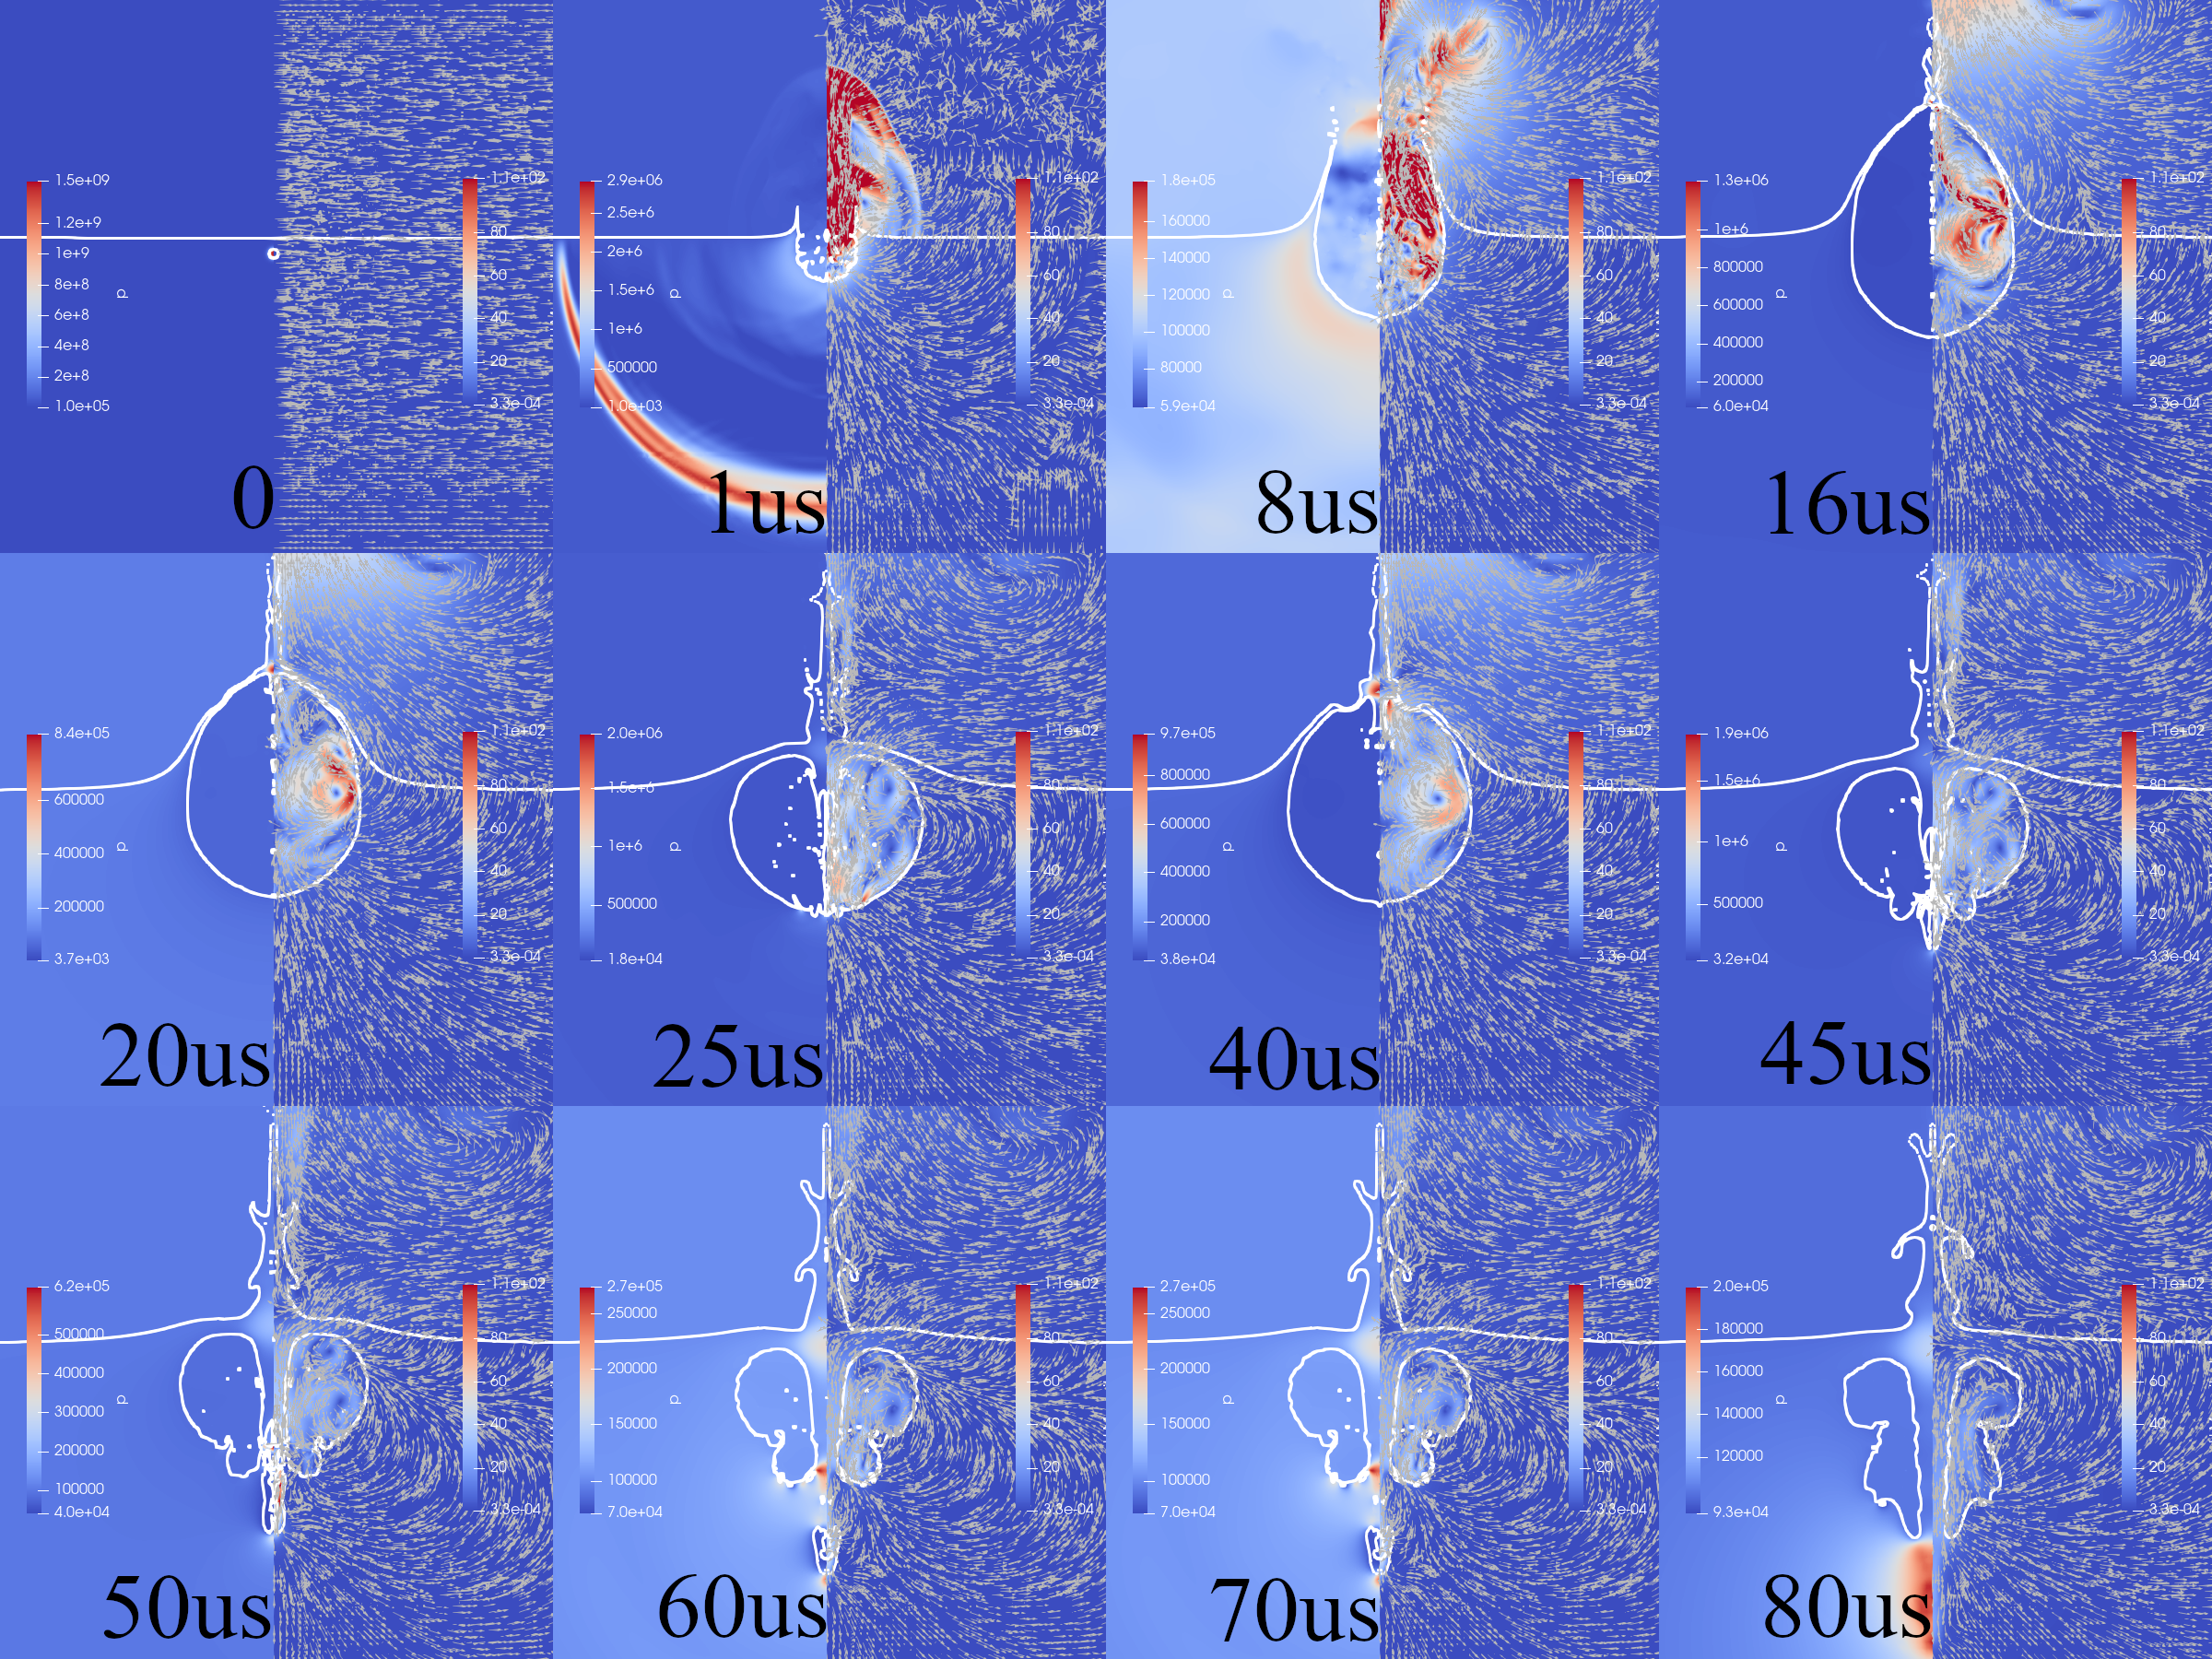
\includegraphics[width=0.9\linewidth]{img/fig3.air0.2.png}
    \caption{空泡距水气界面$\gamma=0.2$情形下的相-速度-压力云图}
    \label{fig3.air0.2pvp}
\end{figure}


图\ref{fig3.air0.2pvp}显示了空泡距水气界面$\gamma=2.0$情形下的相-速度-压力云图。其作为A.爆破式($\gamma\leq 0.3$)空泡与界面的相互作用的典型代表在此处给出其形态学和动力学过程。

图中第一栏第一帧是空泡的初始状态。第二帧($ 1\mu s$)中,空泡膨胀,但因距离界面过近,空泡与自由气体的之间的水体过薄,在推动空泡外水体运动时,形成的拉伸效果将该水体拉断,从而形成图中的爆破效果。因密度和粘度的限制,空泡主要的能量释放方向是近自由面。远自由面方向空泡壁面的运动主要由惯性驱动。从图中速度图可以看到,在爆破形成时,空泡内的气体向自由气体域高速运动。其速度在本帧时刻仍在100m/s数量级,远高于空泡内其他位置的气体。空泡内气体释放到自由气体中后,空泡内外压强行成一次再平衡,这也补充了空泡重生再膨胀的能量。
空泡爆破形成的水尖刺,因空泡气体的推动和空泡推动液体形成的挤压而持续向上运动,形成类似射流的效果。同时可以看到空泡在形成初期辐射的冲击波。因本算法的初始设置更加物理,其对空泡与冲击波的伴生现象相对更加物理,可以用来解释冲击波衰减后的现象,此处不详述。空泡推动形成的辐射状速度场矢量方向,在除空泡下方南极附近辐射指向外,其他方向因冲击波的改造形成指向壁面。
在下一帧($ 8\mu s$)中,空泡的爆破效果愈发明显。自空泡向自由气体域喷射的气体仍高速向竖直上方运动,同时也在横向的推动其本地气体运动。同时水尖刺也在向上延展,并且有横向的向对称轴运动的趋势。空泡横向中心轴以上的位置的速度继续挤压这个水尖刺,促使其继续运动。空泡内部没有形成如上两例中直到低压极限的表现,而是高达一半的大气压,这是与自由气体连通的效果。图中红色高速区域即外界气体进入空泡内部的表现。
在第四帧($ 16\mu s$)中,上述的尖刺结构横向运动后撞击,并形成向上和向下的射流的物质释放通道。此时场内的速度矢量仍多数指向自由面。空泡在水体内的膨胀,使得空泡横向中心轴以上部分仍挤压这个尖刺结构。同时可以看到,进入空泡内部的自由域气体在空泡内部形成特殊的高速读结构,其会冲击空泡壁面,造成一定的形变。此时空泡内的气体再次封闭,形成卵状结构。

在第二栏第一帧($20 \mu s$)中,空泡封闭后形成的双向射流继续向双方向发展。而封闭的尖刺结构因空泡推动和后续速度的挤压,在空泡正上方,也就是碰撞区域形成一个高压点。这个高压区域将继续推动双向射流的发展。而因为空泡的封闭,外来气体的速度撞击,以及水体惯性运动形成的空泡的继续膨胀,空泡内部压强减小,形成空泡的收缩趋势。因密度和粘度的问题,空泡在压强差驱动下的收缩仍最先发生在近自由面,也就是空泡的上方壁面最先开始收缩,即本栏第二帧($25 \mu s$)。此时的空泡下部仍在继续膨胀,空泡上方因压差形成尖刺结构的内凹,并由此将射流分裂出类似皇冠射流的结构,上射流形成多层结构。射流根部空泡上部的高压将推动空泡和射流形状的继续演化,即下一帧($40 \mu s$)中,上射流形成类似竖叉式结构,而下射流继续向射流相对壁面运动。而此时空泡上方的水层因空泡的收缩和速度的汇集,以及再次加厚,成为水射流稳定的物质来源。最后一帧($45 \mu s$)中,下射流击穿空泡,使空泡产生凸起结构,为接下来的双层空泡结构奠定基础。

在第三栏($ 50\mu s$,$60 \mu s$,$70 \mu s$,$ 80\mu s$)中,主要展示了远离自由面,指向空泡内部的水射流贯穿空泡的动力学过程。因射流的高速运动,射流裹带空泡气体向下方向运动,形成了特殊的双层空泡结构。即空泡部分在原位置,一部分突破的空泡位置的下方。在这个过程中空泡的泡内气体的物质量充足,没有发生溃灭现象。而且,射流在这个过程中因后续速度的继续挤压,仍旧向上延展和变形。注意,在实际中,因重力的作用,上射流会更早地进入回退进程,此处不讨论。

在本例中,空泡与自由气体之间的水体层过薄,在膨胀初期即破裂,由此形成这种空泡的爆破机制。空泡膨胀时推动液体向其上部运动,形成尖刺结构,这种结构在后续水体的推动下相互碰撞,继而产生上下两股射流。因空泡破裂与外界压强发生平衡,所以空泡最后没有形成溃灭现象,而是被射流推动形成多层结构。


\begin{figure}[h]
    \centering
    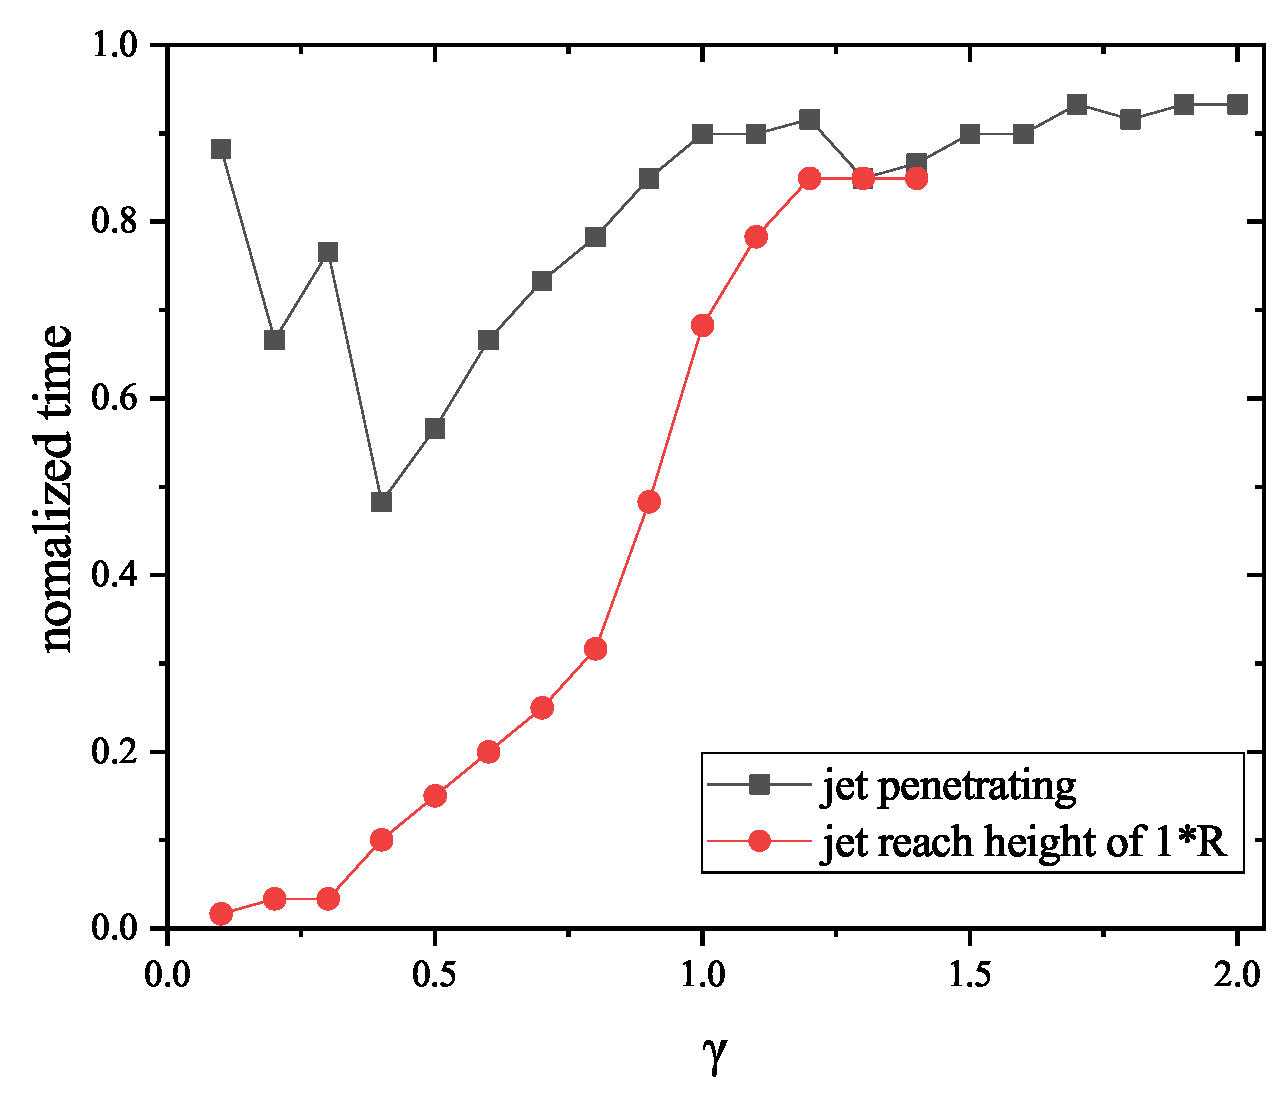
\includegraphics[width=0.6\linewidth]{img/fig3.airjettime.eps}
    \caption[水气界面附近情景下射流击穿时间和上射流到达一倍半径的归一化时间]{空泡距水气界面不同相对距离情形下的下射流击穿时间和上射流到达一倍半径距离的归一化时间。黑色是射流击穿时间,红色是上射流到达一杯空泡半径距离时间。}
    \label{fig3.airjettime}
\end{figure}

在共20组结果中,每组都发生了非对称的溃灭现象,即射流。为了对空泡与自由面的相互作用和射流的强度进行某种量化,将指向空泡内部的射流到达对立壁面的时间作统一的归一化处理,即$T_\mathrm{nomalizd penetrating}=t_\mathrm{penetrating}/t_\mathrm{freeosc}$。其中$t_\mathrm{penetrating}$指空泡射流到达对立面的时间, $t_\mathrm{penetrating}$指上文中空泡在自由域的体积最小时间。同时我们对上射流的更关注其形成后的速度,也定义了一个能间接反应其速度的归一化时间,$T_\mathrm{nomalizd-jet-reach}=t_\mathrm{jet-reach}/t_\mathrm{freeosc}$。其中$t_\mathrm{jet-reach}$指空泡的上射流到达1倍自由域内空泡最大泡半径$R=330mm $的时间。

从图\ref{fig3.airjettime}中可以看到,下射流的击穿空泡时间在$\gamma \geq 0.4$范围中,是随着$\gamma $的增长而变晚的。在$\gamma \leq 0.3$中因形成了爆破式相互作用,其射流形成机制与其他情形不同,故而较晚。但整个过程中形成的上射流,即指向自由气体域的射流到达一倍R的时间是越来越晚的,就表明上射流的初始速度是随着空泡与界面距离的增加而减弱的。因$\gamma \geq 1.5$没有形成向上的水射流,而仅是凸起形态,此处不涉及。


\begin{figure}[h]
    \centering
    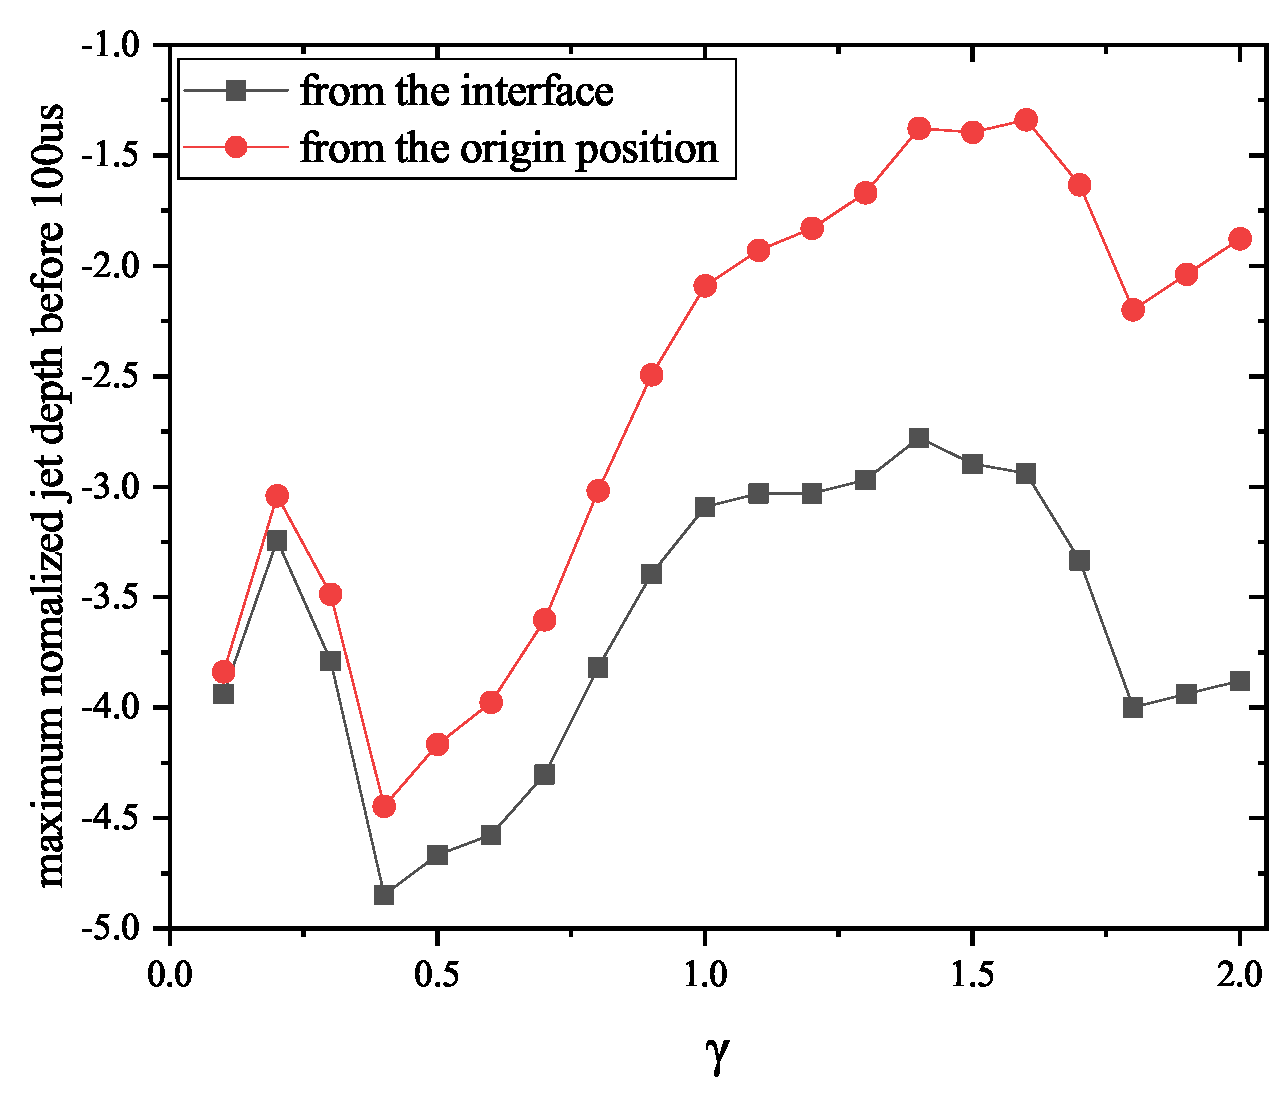
\includegraphics[width=0.6\linewidth]{img/fig3.airdistance.eps}
    \caption[空泡距水气界面不同相对距离情形下的归一化射流深度]{空泡距水气界面不同相对距离情形下的归一化射流深度。黑线是以界面为基准,测量的深度。红色是以空泡初始位置为基准形成的深度。负值表示深度。}
    \label{fig3.airdistance}
\end{figure}

向下的射流,即击穿空泡的射流,在水中受到水的阻滞,其传播距离有限。通常在较长时间范围内,通过空泡的多次脉动,其可以达到十几倍R的距离。此处我们只关注其在第一个生命周期结束后直到第二次生命周期结束前的$100\mu s $内传播的最远距离。从图\ref{fig3.airdistance}中,我们可以看到,在B.皇冠射流式($0.4\leq\gamma\leq 1.4$)相互作用范围内,空泡的射流深度是随着$\gamma $的增加而变浅的,反映了自由面对空泡的弹弓效应是随着自由面与空泡初始位置的距离变大而减弱的。在C.突起式$\gamma\geq 1.5$)相互作用范围内,其存在一个过渡的区域和一个彻底的凸起式的区域,但其深度确实在一定范围内比某些情况深。而在A.爆破式($\gamma\leq 0.3$)范围内,因涉及到压力再平衡,其溃灭烈度远小于未连通的其他两种情况,从而其射流深度也小于B的某些情况。









\subsection{单空泡在水油界面附近的脉动}
硅油是一种稳定无毒的有机油类。其在工业上应用广泛。特别的,通常因其可调节粘度,而作为一种研究空泡受粘度影响的环境液体。本文选取一种实验室易获得的硅油($\mathrm{C_2H_6OSi}$)作为液-液界面情况的第三相,见图\ref{fig:interface}。
这种硅油的具体性质已在在上文中给出(表\ref{tab:3.1})。其本身的实际物理参数表现为一种高粘性液体。如果要针对某一个具体的特性研究其对空泡的影响,可以设置实际实验上难以获得的物性参数。但此处仍选择其真实物理性质。

通常激光空泡的环境液体因为粘性增加,会加剧了空泡脉动的能量耗损,从而造成空泡脉动现象的减弱,包括生存周期变小和射流现象的减弱。而高粘液体作为流域的一部分,也会对空泡造成相似的影响。因兼具可流动和高粘度的边界特性,水油界面附近水体内产生的空泡,会表现出兼具自由界面和固体界面附近的特性。

\begin{figure}[h]
    \centering
    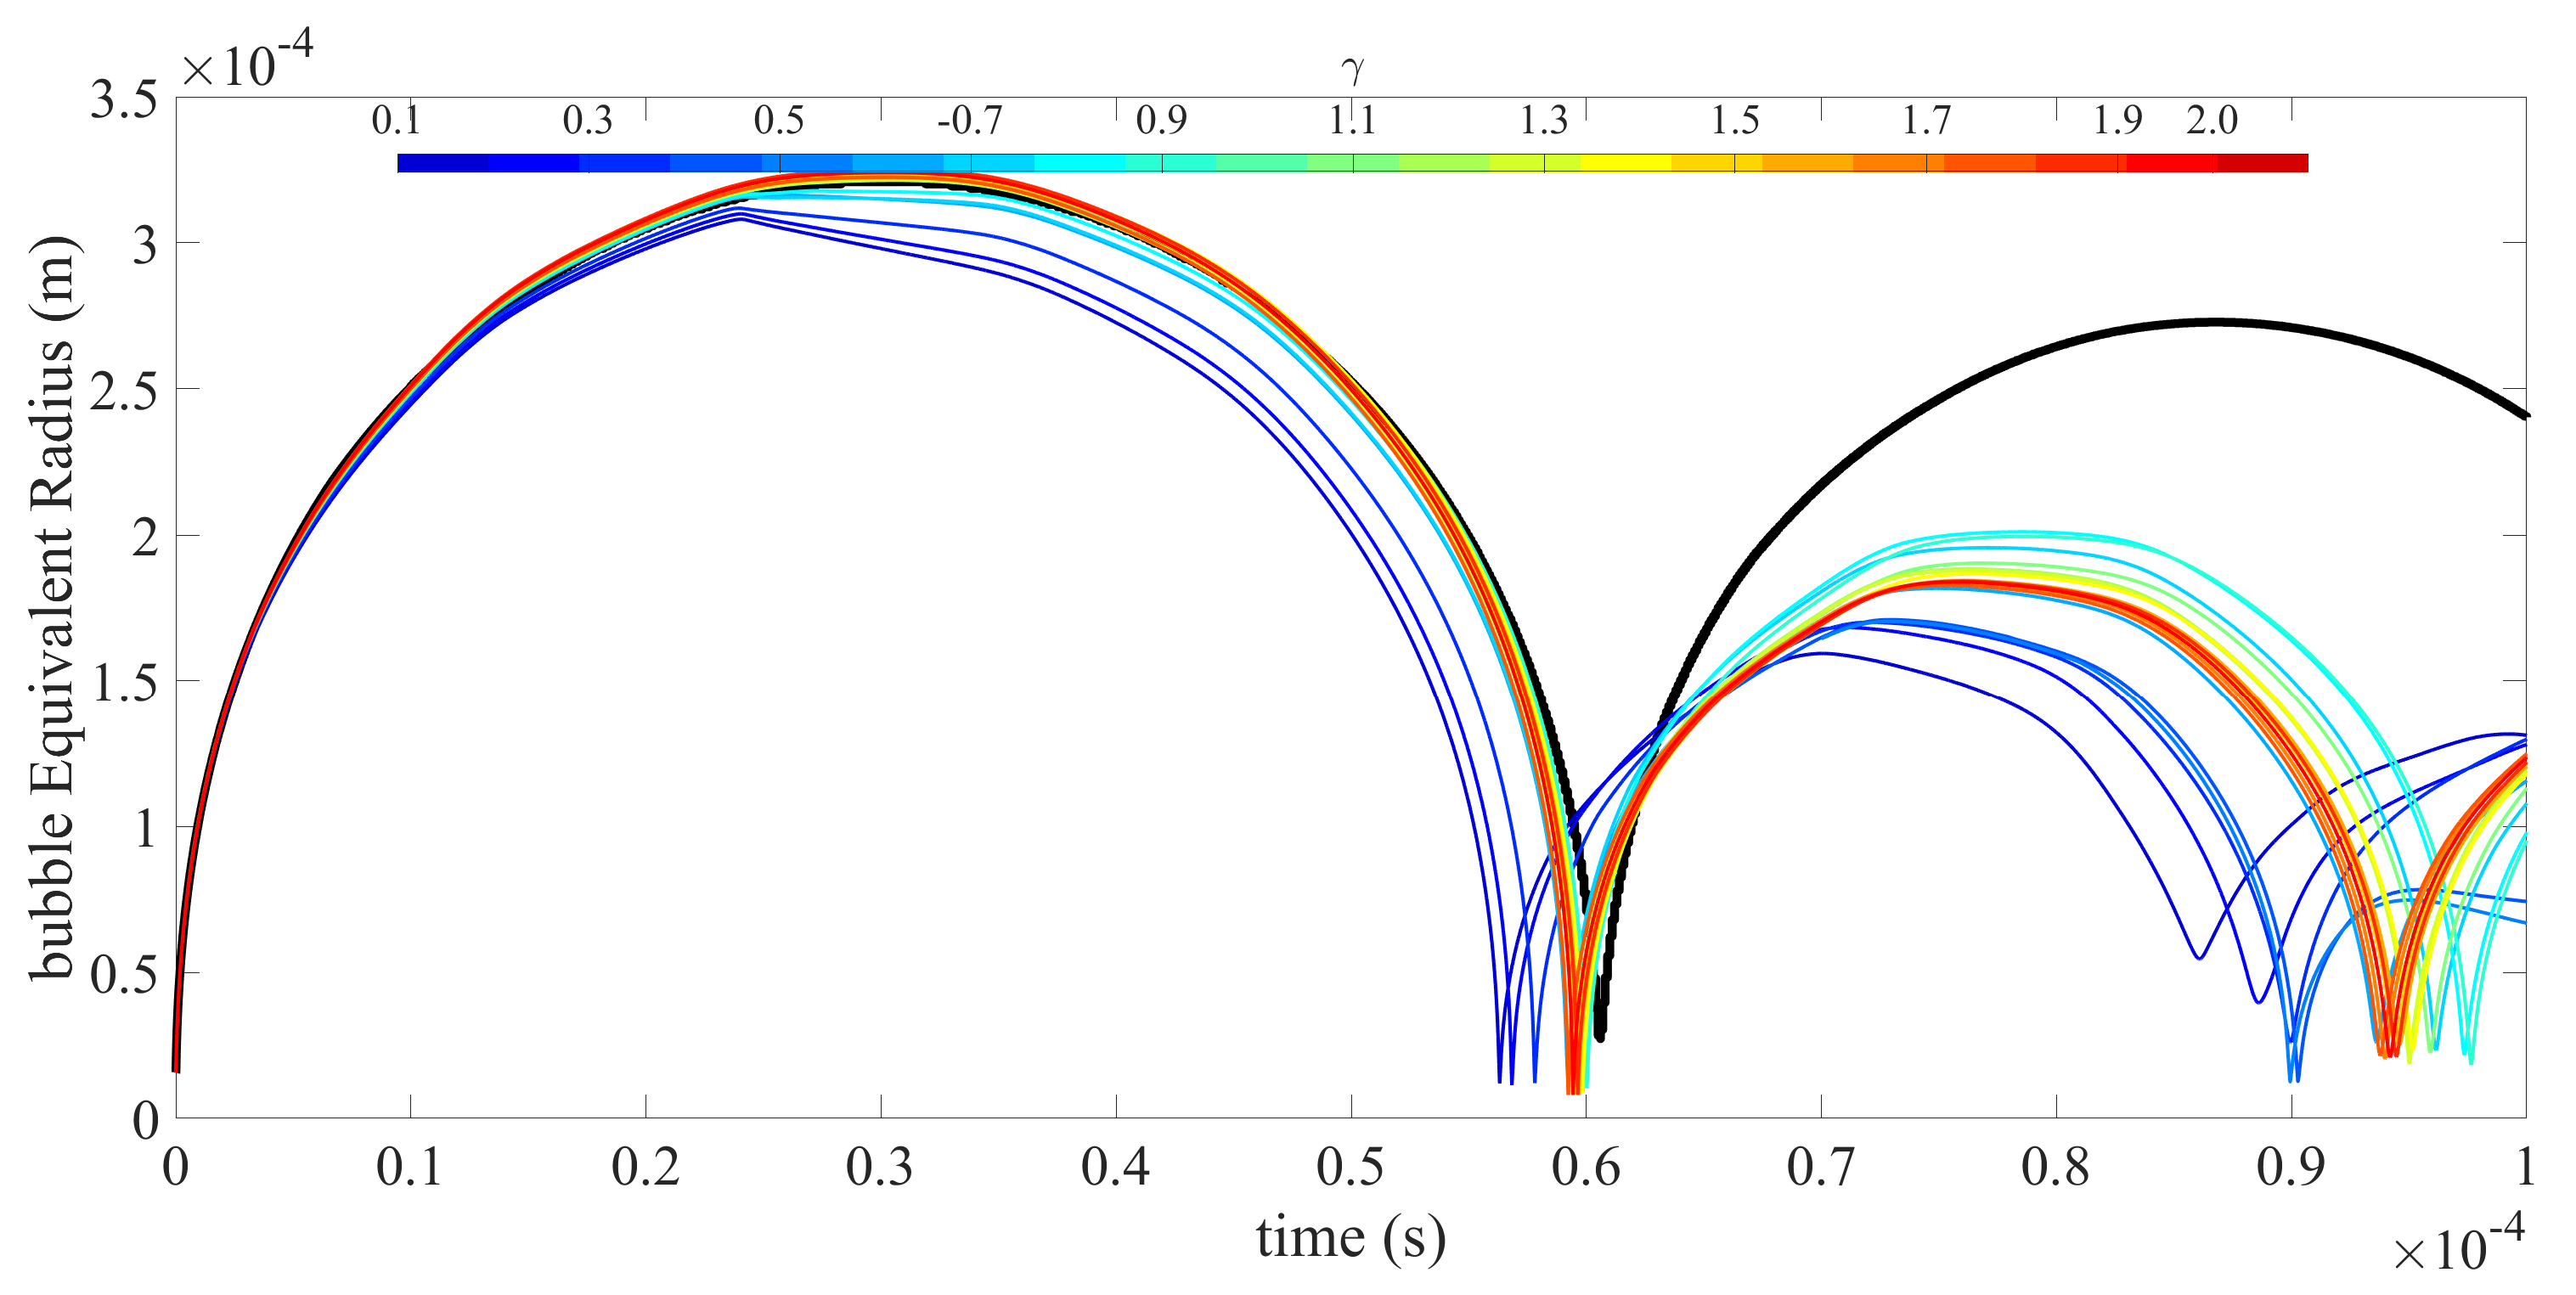
\includegraphics[width=1\linewidth]{img/fig3.oilradius.eps}
    \caption[空泡距水-硅油界面不同相对距离情形下的泡半径对比图]{空泡距水-硅油界面不同相对距离情形下的泡半径对比图,图中黑色实线为自由域中的模拟结果。}
    \label{fig3.oilradius}
\end{figure}

\begin{figure}[H]
    \centering
    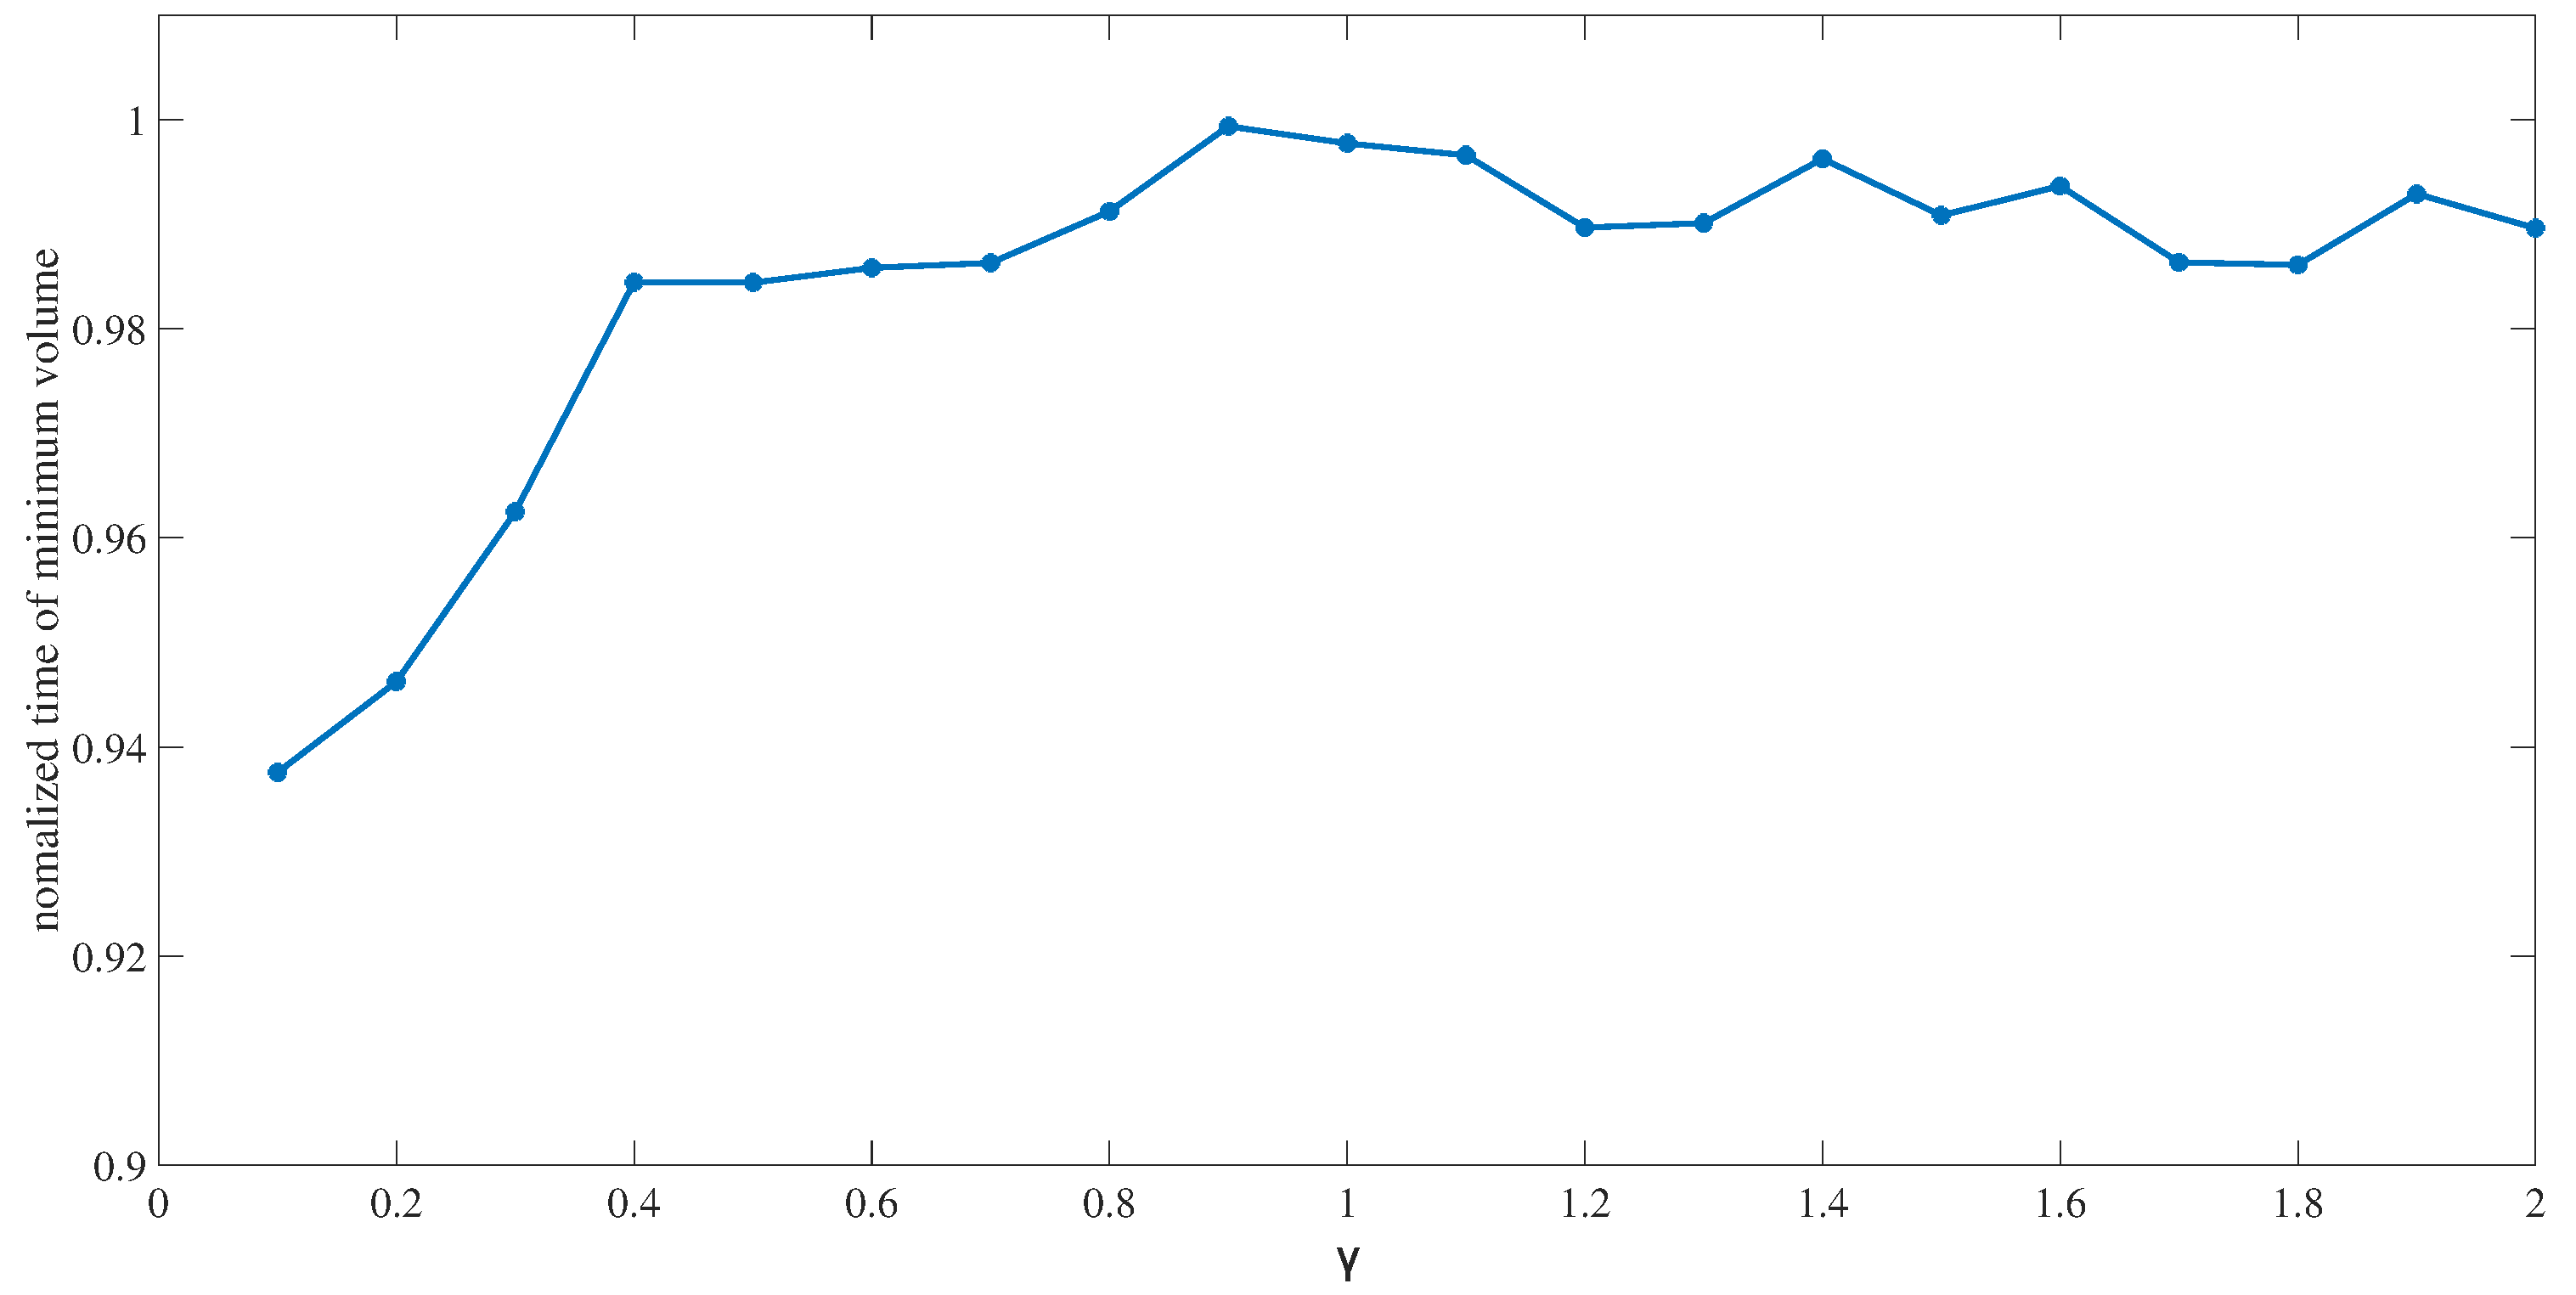
\includegraphics[width=0.9\linewidth]{img/oilclpstime.eps}
    \caption[水-油界面附近空泡的归一化溃灭时间]{水-油界面附近空泡的归一化溃灭时间。归一化时间通过模拟计算中获得的体积最小时间除以自由域中的体积最小时间60.06$\mu s $获得。}
    \label{fig:oilcolltime}
\end{figure}

图\ref{fig3.oilradius}中给出了空泡与水油界面在不同相对距离$\gamma$处的体积等效半径对比图。可以看到,在$\gamma$越大,也就是越接近自由的情况下,空泡的体积等效半径越接近在自由域中的脉动。
在$\gamma\leq 0.3$,也就是空泡在界面附近时,空泡的半径在膨胀到最大泡半径之前,大约$24\,\mu s$左右开始出现明显地受压迫而减缓增长加速溃灭的现象。这是因为由于与界面距离过近,膨胀过程中推动密度高,粘性高的硅油而耗费能量,并因张力影响而提前回弹。从图\ref{fig:oilcolltime}中通过归一化放大溃灭时间的差异后,可以看到空泡的生存时间形成明显的阶段性区分。$\gamma\leq 0.3$ 时,溃灭时间形成一个明显的上升趋势。$\gamma$其脉动时间越接近自由脉动。
$0.4\leq\gamma\leq 0.6$时,溃灭时间形成一个平台。
$\gamma\geq 0.7$时,溃灭时间形成一个波动曲线。这三个阶段的体积等效半径的变化对应了不同的空泡脉动形式。通过对其场内各向异性的性质研究,我们可以获得更细致的信息。



从空泡自身溃灭形式的角度区分,空泡总体上可以分为两种溃灭模式,断裂式($\gamma\leq 0.6$)和射流式($\gamma\geq 0.7$)。断裂式指空泡溃灭时,横向的受到冲击,从而形成接近界面和远离界面的两部分。射流式指空泡在溃灭后期纵向的形成射流的趋势,并在随后的回弹中表现出强射流的溃灭。其中断裂式又可以细分为:A.断裂接触式($\gamma\leq 0.3$)和B.断裂射流式($0.4\leq\gamma\leq 0.6$)。A.断裂接触式指空泡在溃灭时,其横向的冲击在空泡内部没有形成纵向的击穿空泡的射流,而是以空泡贴近界面的方式影响界面。而B.断裂射流式指空泡在横向断裂时,同时产生了射向界面的射流了,并击穿空泡射向界面。
下文中将结合三种情况的典型案例($\gamma= 0.1$,$\gamma= 0.5$,$\gamma= 2.0$)的相-速度-压力图详细地解释几种机制的动力学过程。


\begin{figure}[h]
    \centering
    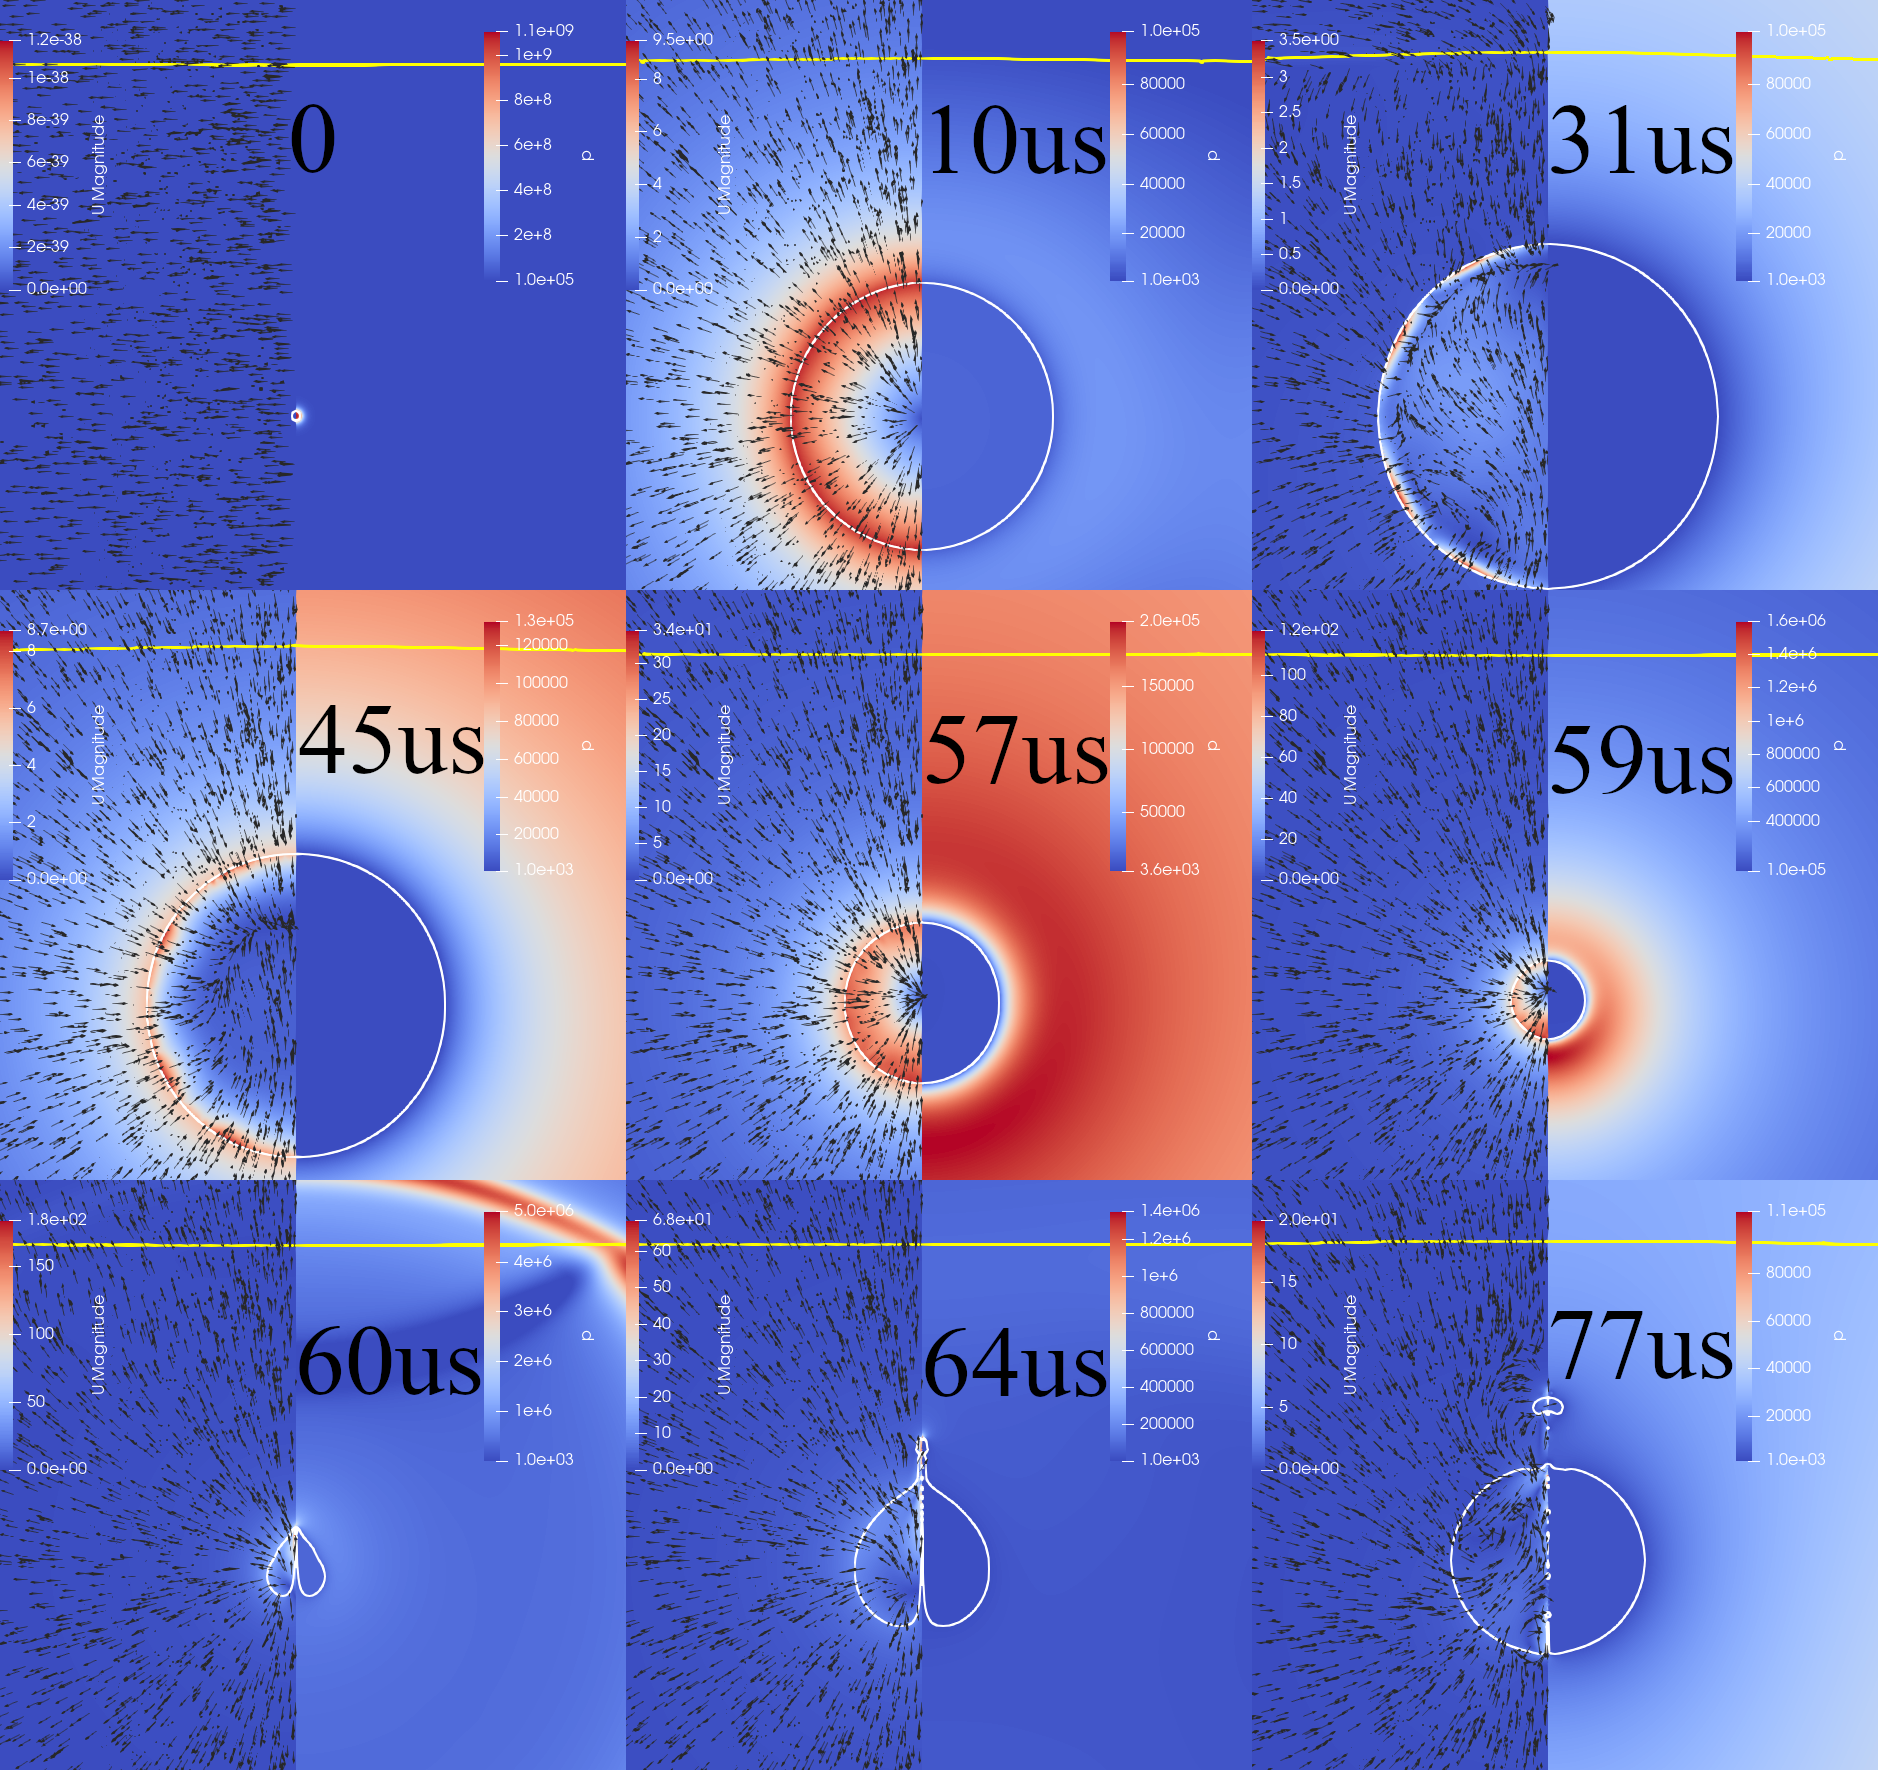
\includegraphics[width=0.9\linewidth]{img/fig3.oil.2.0.png}
    \caption[空泡距水-硅油界面$\gamma = 2.0$情形下的相-速度-压力云图]{空泡距水-硅油界面$\gamma = 2.0$情形下的相-速度-压力云图。图中黄线代表水油界面。界面以上为油,界面以下为水。每一帧的左侧是流域的速度场(单位m/s),右侧是压力场(单位Pa)。白色线表示气体空泡的轮廓。黑色箭头是速度场的方向。该帧的具体时刻标注在压力场的空白处。以下三个相-速度-压力云图按照同样的标注方式作图。}
    \label{fig3.oil2.0}
\end{figure}

图\ref{fig3.oil2.0}显示了空泡距水-硅油界面$\gamma = 2.0$情形下的相-速度-压力云图。第一帧表示该情景下的初始状态,即0时刻。第二帧($10\mu s$)中,显示了空泡的初始膨胀阶段。此时空泡壁面在向外急剧的扩张,速度仍近100m/s,场内的速度矢量自空泡初始位置呈放射状发展。这是由于空泡在初始时刻向外释放的冲击波几何传播,推动当地液体实现的。而由于空泡膨胀超出了其均衡半径,此时其泡内压降到了环境压以下。在膨胀一段时间后,空泡在$31\mu s$左右达到最大泡半径。可以看到第三帧中空泡外已经形成指向空泡内运动的速度。而空泡内部与自由域的最大泡半径时空泡各向同的向内收缩不同,此时空泡受界面影响形成局部的压力梯度,空泡内部形成自远离界面到靠近壁面方向的速度。速度的终点在靠近空泡上壁面附近。这也为射流的形成埋下伏笔。

在第二栏中,显示了空泡收缩的过程。其中第一帧($45\mu s$)中上述的速度终点区域向泡中心移动,稍微远离了空泡壁面。空泡壁面的速度达到了约8m/s。在下一帧($57\mu s$)中速度终点的位置持续向中心移动,但仍处于空泡内部的上方位置。全流域受泡外压的驱动向空泡运动,同时因速度提升和几何限制的原因,空泡壁外的压力受到一定的提升,并作用于速度的继续提升。而这时,空泡壁面速度已经达到30m/s以上。随后在第三帧($59\mu s$)中,约两微秒的时间,空泡壁面的速度已经达到了120m/s。而上述的压力提升在空泡的下方,也就是远离水油界面的位置,产生了更高的压强。这为空泡自空泡下方形成向上的射流提供了必要条件。

第三栏中,就显示了空泡的射流击穿,及其后续的再膨胀过程。第一帧($60\mu s$)中,空泡非球型溃灭,空泡向外辐射了一个冲击波。而其因非球型溃灭形成的击穿射流,此时也击穿空泡近界面的壁面。这个射流的速度在180m/s左右。辐射的冲击波在界面处发生了透射和发射。在射流击穿后($64\mu s$)继续向界面移动并持续减速,空泡继续膨胀。在第($77\mu s$)图像中显示,射流裹带的气体因速度减小,以及表面张力和空泡收缩的共同作用,被留在原地成为一个独立的小空泡。而大空泡将继续其脉动生命周期。

在本例中,空泡的脉动表现出接近自由域的脉动性质,同时也产生了受液面影响的射流。这与使用章节\ref{chapter1.2.2.2}中
$\bm\zeta=0.195 \gamma^{-2}\left(\rho_{1}-\rho_{2}\right)\left(\rho_{1}+\rho_{2}\right)^{-1} \boldsymbol{n}$计算获得的$\bm\zeta$预言的矢量方向和射流强度相一致。




\begin{figure}[h]
    \centering
    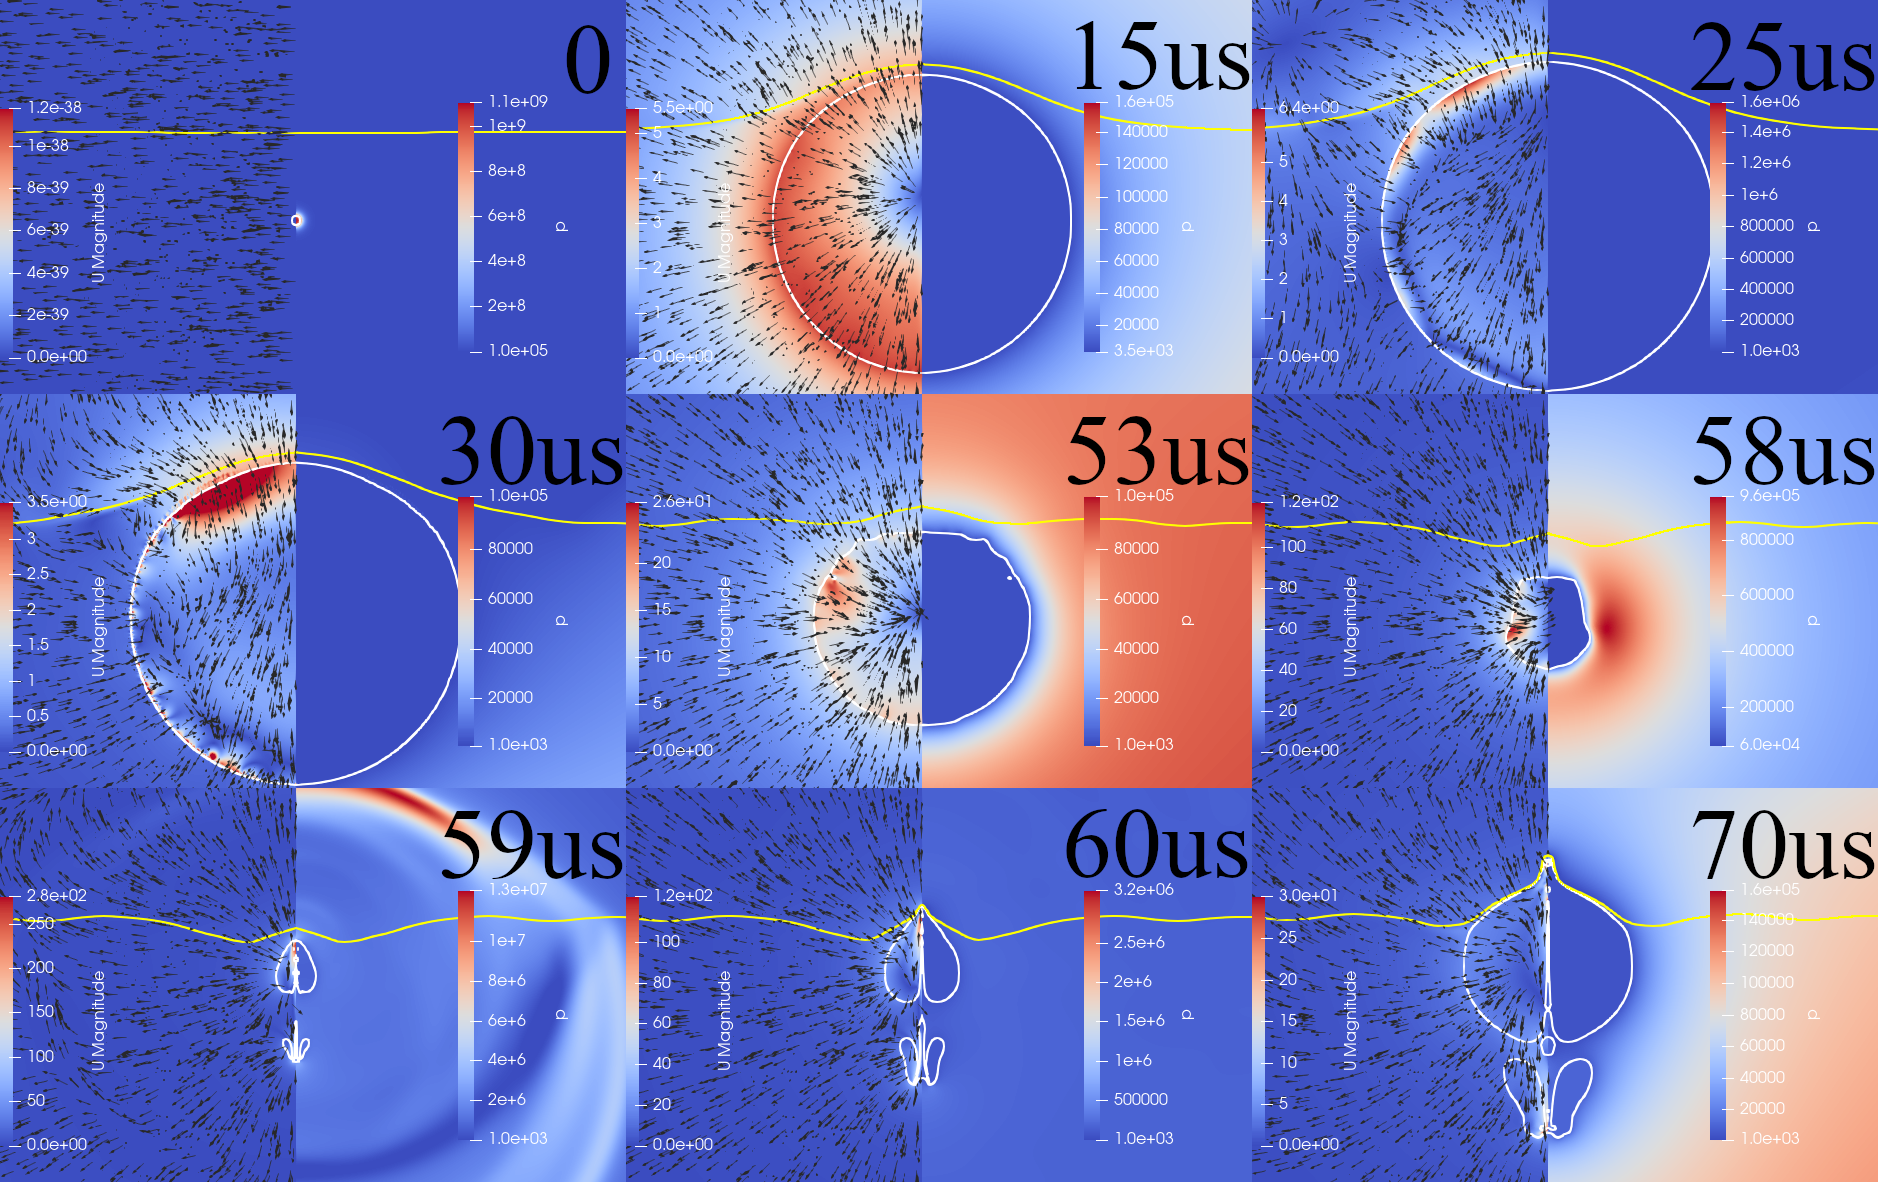
\includegraphics[width=0.9\linewidth]{img/fig3.oil.0.5.png}
    \caption{空泡距水-硅油界面$\gamma = 0.5$情形下的相-速度-压力云图}
    \label{fig3.oil0.5}
\end{figure}

图\ref{fig3.oil0.5}显示了空泡距水-硅油界面$\gamma = 0.5$情形下的相-速度-压力云图。
第一栏第一帧显示了空泡的初始状态。第二帧($ 15\mu s$)显示空泡的初始膨胀阶段。在这帧中,空泡向外辐射状的膨胀。在壁面到达界面附近时,推动界面变形。因硅油更重更粘,其流动较水的流动变化更满,速度更慢。从而使空泡更倾向于在远离界面方向释放空泡能量。也就是在空泡远离界面的壁面的速度相较与界面相对的壁面速度更快。因泡内低压少物质的特点,泡内的速度中心也就是零速度点,约等于空泡南北极速度的中心点,位置向上移动到靠近壁面处。在第三帧($ 25\mu s$)中,空泡远离界面的下壁面因水的惯性仍在向外膨胀中。而界面附近处的上壁面因其速度一直慢于下壁面,而且界面因张力而倾向于恢复其初始状态,使上壁面相比下壁面更早的进入到收缩周期。此处就对应着图\ref{fig3.oilradius}中的转折部分。进而空泡形成自界面向水体内的速度。

在第二栏中,($30\mu s$)帧显示了空泡下壁面膨胀到最大的情景。上壁面持续向内收缩,下壁面内的气体有向外膨胀的速度,但泡外的水已经开始进入回归进程。下一帧($ 53\mu s$)中,空泡持续收缩,并且在靠近界面的上壁面发生平化现象。而界面则将空泡膨胀形成的挤压和拉伸以剪切波的形式传播了出去,形成了界面特殊的形变。而此时,空泡的速度终点位置已经回到空泡的初始位置附近。特别的,我们可以注意到,在空泡水平轴以上和平化壁面以下位置,形成一片高速度区域。这片高速度区域是在界面回弹的基础上叠加收缩形成的。在($ 58\mu s$)时其非常明显的形成一个向内凹陷的区域。因为其对应着速度终点的位置,域内的流体物质向速度终点汇集,继而引发该位置的高压和高速度。而高压高速度将变成壁面的驱动力,以完成下一栏的动力学表现。

第三栏中,第一帧($ 59\mu s$)表示了上栏第三帧的下一微秒的状态。此时空泡,因高压高速区域驱动壁面运动,继而撞击,形成水锤辐射高压并将空泡自撞击位置切断。水锤压在弯曲界面处发生复杂的反射和投射,形成特殊的压力场。而因为撞击前特殊的空泡形状,撞击后形成特殊形状的水射流,即在靠近壁面的部分中形成单束水射流,而在远离界面的部分中形成辐射状的圆锥射流。从而使上部分的残留空泡内形成单射流撞击。在下部分残留空泡形成特殊而花托状。下一帧($ 60\mu s$)则更加清晰,单射流击穿上部分空泡,并对界面造成尖刺状形变。而空泡也随着射流向界面运动,形成心形$\spadesuit$射流。下部分空泡则明显的形成了一种圆锥状溅射。在最后一帧$ 70\mu s$)中,射流裹带空泡气体向界面运动到失去速度,而因空泡膨胀射流失去后续水射流的填充,继而在空泡内发生断裂,成小液滴。而下部空泡的膨胀也挤压使圆锥状射流合并和脱落。

这种情况下,空泡膨胀时会推动水油界面移动和变形,油体会对空泡壁面移动进行减速和推动空泡重心位置变动。在空泡收缩时,界面同样使空泡壁面发生变形,从而形成特殊的撞击溃灭结构,进而使空泡横向的撞击溃灭,分裂成两部分,其中靠近界面的一部分被射流击穿,进而射流推动界面运动。

\begin{figure}[h]
    \centering
    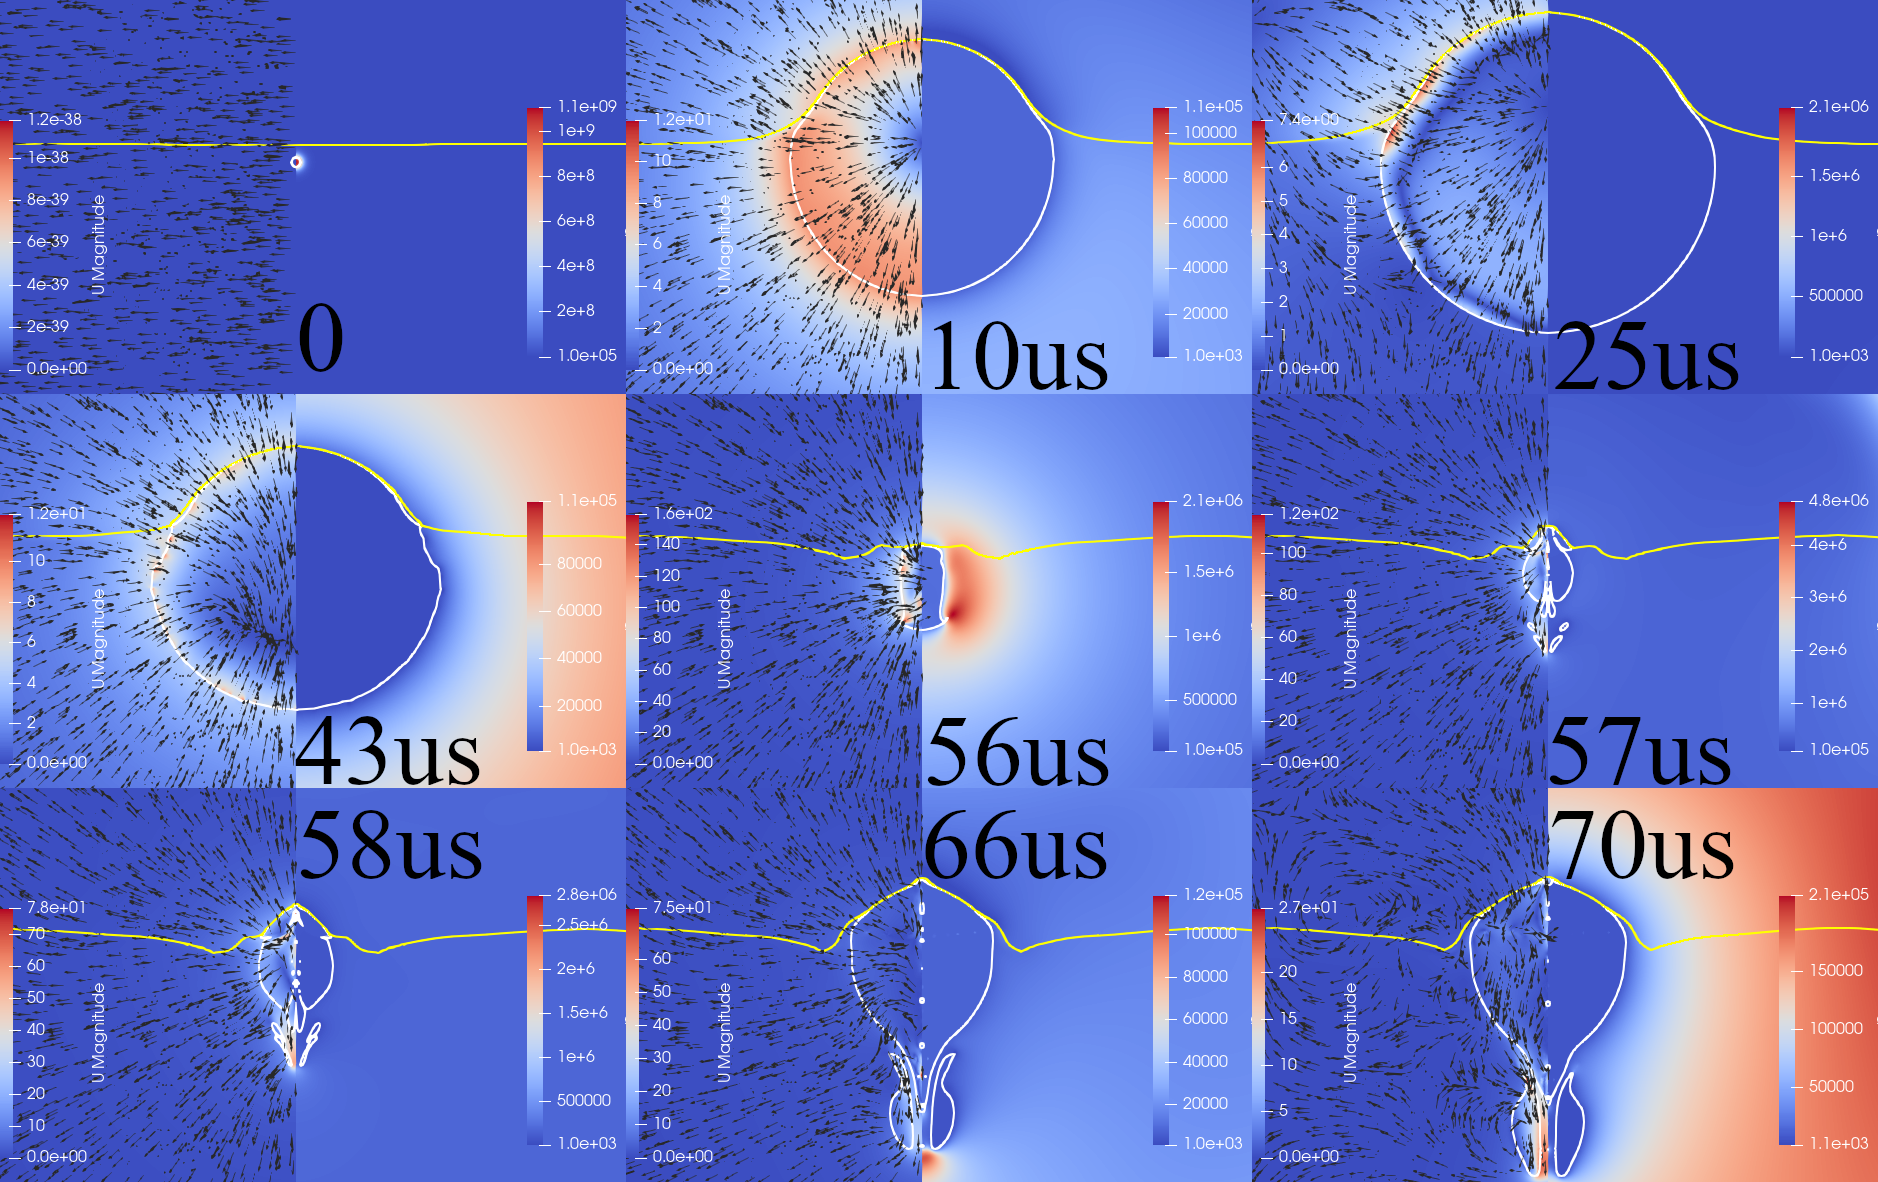
\includegraphics[width=0.9\linewidth]{img/fig3.oil.0.1.png}
    \caption{空泡距水-硅油界面$\gamma = 0.1$情形下的相-速度-压力云图}
    \label{fig3.oil0.1}
\end{figure}

图\ref{fig3.oil0.1}显示了空泡距水-硅油界面$\gamma = 0.1$情形下的相-速度-压力云图。这种情况下,空泡和界面发生最强烈的相互作用。该图第一帧仍是初始状态。第二帧($10\mu s$)中,空泡辐射式膨胀,但空泡膨胀使上壁面在更早期直接接触水油界面。空泡的膨胀受界面的明显约束,从而空泡的下壁面运动速度快于与界面相接触的上壁面。于是形成空泡近界面的部分平均半径小于其下半部分。这样就使空泡的速度零点的位置更靠上,甚至超过空泡初始位置。在第三帧($25\mu s$)中,空泡的速度零点明显上移到原界面位置之上。此时其处于最大泡半径时刻,远离界面的壁面仍在向外低速膨胀,而近界面的上壁面已经开始收缩。此时对应图\ref{fig3.oilradius}中的明显转折。而可以注意到,在界面-水体-空泡的交接处,此时形成速度高区,这也使后续此处发生特殊的形变。而因上下不均衡的膨胀,使此时空泡下方的半径超过自由域的最大泡半径。

随后在收缩阶段的第二栏第一帧($43\mu s$)中,空泡收缩时其速度零点,或者速度终点在空泡的下半部分。这是空泡近界面的上壁面的收缩早,速度快导致的。而因为这个速度终点的位置低于中间形成的突起部分,使得突起上下的壁面保持这种相位领先直到空泡溃灭。于是产生下一帧中($56\mu s$)空泡上下两个凹陷。而此时空泡的收缩使界面回弹到近初始位置,也对界面造成形变。值得注意的是,此帧中空泡的下半部分因形成凹陷结构,这种结构的收缩形成水体的撞击,从而形成辐射冲击波。这种冲击波有加速了空泡的溃灭过程。因形成了两个凹陷结构,在($57\mu s$)中,空泡的溃灭形成两处断裂。这点可以从空泡分裂成三个大部分看出。其中上、中两个大部分中间形成了一个锥形射流隔断中,从而使上部分形成一个环形空泡。而中间部分,则被自下而上的环形射流击穿,并向上突入环形空泡内部,推动界面变形。而下部分,则因凹陷的撞击和下突起的运动,也被截断成两部分。一部分随圆锥射流进入中大部分空泡内部,下半部分被射流裹带向远离界面的方向运动。

随着空泡的继续脉动,在($58\mu s$)也就是第三栏第一帧中,上中两个大部分合并成一个新的大空泡,直接接触界面并继续膨胀。而下大部分由于分成了两部分,其进入大空泡内部的一部分因射流的断裂而与大空泡融合,并接续的向外膨胀。另外部分则逐渐结合在一起形成了新的空泡。于是如第二帧($66\mu s$)中,空泡重新组合成两个大空泡,其中的主体部分大空泡与壁面接触而继续膨胀,并且其中深入的到另一个空泡的尾巴持续收缩。而另一个空泡则膨胀,一挤压尾巴回归,二挤压尾巴断裂部分的向外加速。在最后一帧($70\mu s$)中,主体空泡开始收缩,另一个空泡被动变形。

在本例中,空泡初始位置极为靠近界面,导致其动力学受硅油影响较大。其膨胀和收缩均受到限制,从而形成特殊的溃灭形态,在横向壁面撞击后,空泡被割裂成几个有关系的个体。

在以上三种情况中,射流机制贯穿全程。空泡最后都发生了非球形溃灭,也就是被各种形式的射流击穿。除了在$\gamma\leq0.3$中,其他每种情况都发生了空泡产生的射流射向界面,有的还有射流撞击界面发生。



\begin{figure}[h]
    \centering
    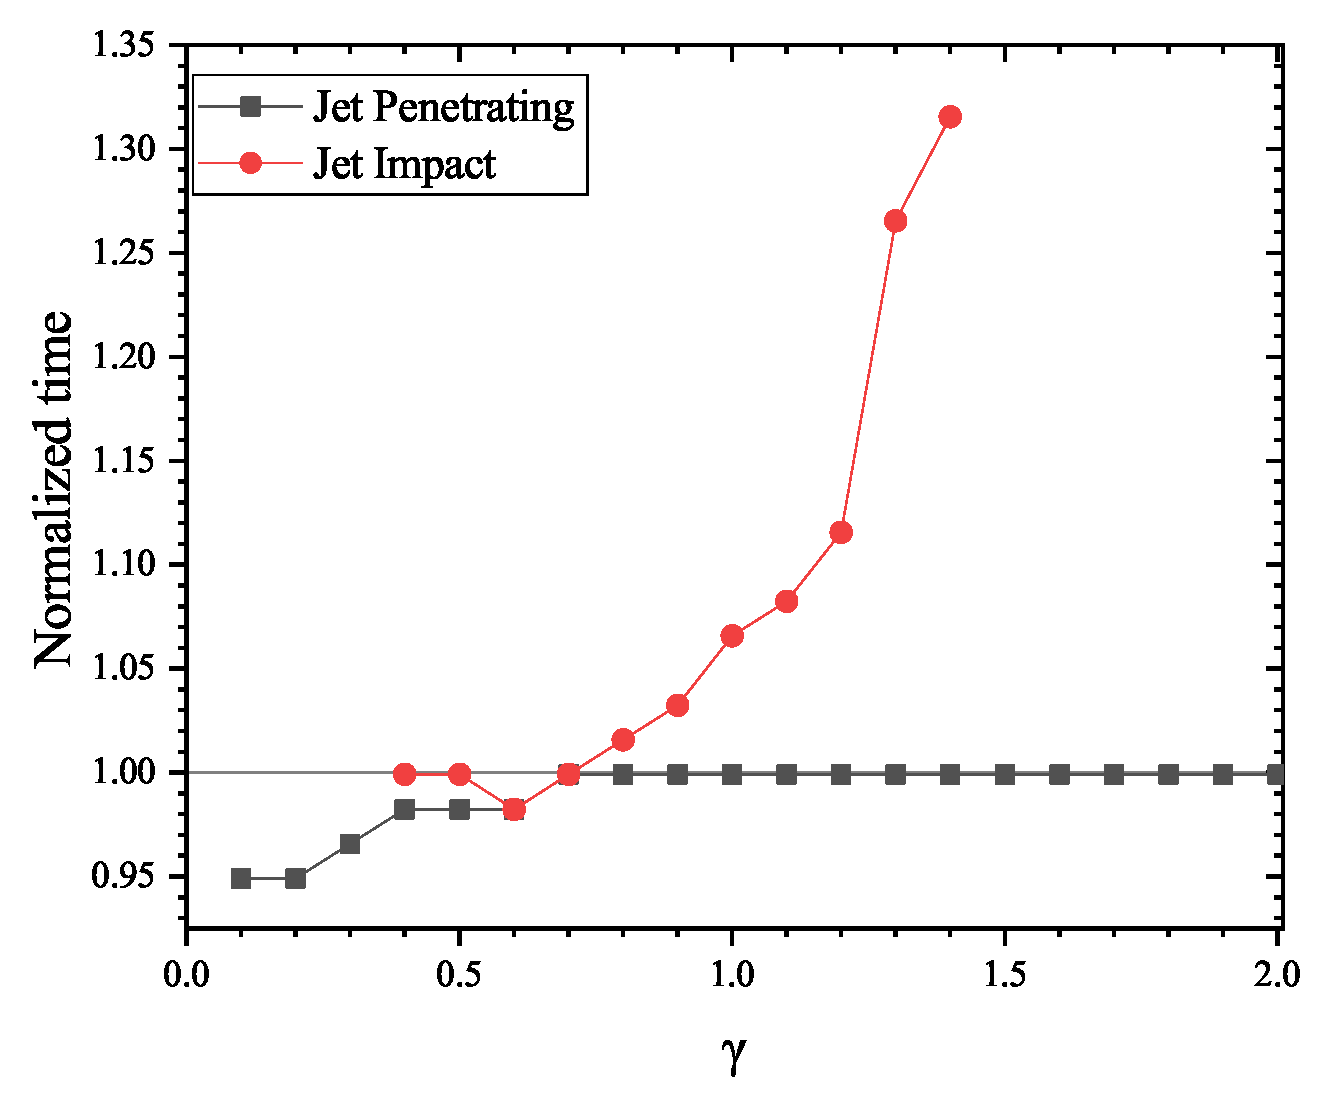
\includegraphics[width=0.6\linewidth]{img/fig3.oiljettime.eps}
    \caption{空泡距水-硅油界面不同相对距离情形下的射流击穿时间}
    \label{fig3.oiljettime}
\end{figure}
图\ref{fig3.oiljettime}中给出了,射流击穿空泡的时间和射流撞击界面的时间。
考虑到因空泡的膨胀和收缩使界面位置发生了变化,此处定义射流撞击时间为射流到达界面原位置的时间。从图中我们可以看到,在1$\mu s$的采样误差内,$\gamma\geq0.7$时的空泡的射流击穿时间几乎一致。在$\gamma<0.7$时,其撞击时间是递增的。而射流撞击时间上,$\gamma\leq0.3$时没有发生常规的射流和射流撞击,$\gamma\geq1.4$时,空泡的射流没有达到界面就丧失速度,无法到达界面位置。

从界面视角来看,空泡的脉动对其外形进行了改造。产生了类似自由界面的突起等情况。

\begin{figure}[h]
    \centering
    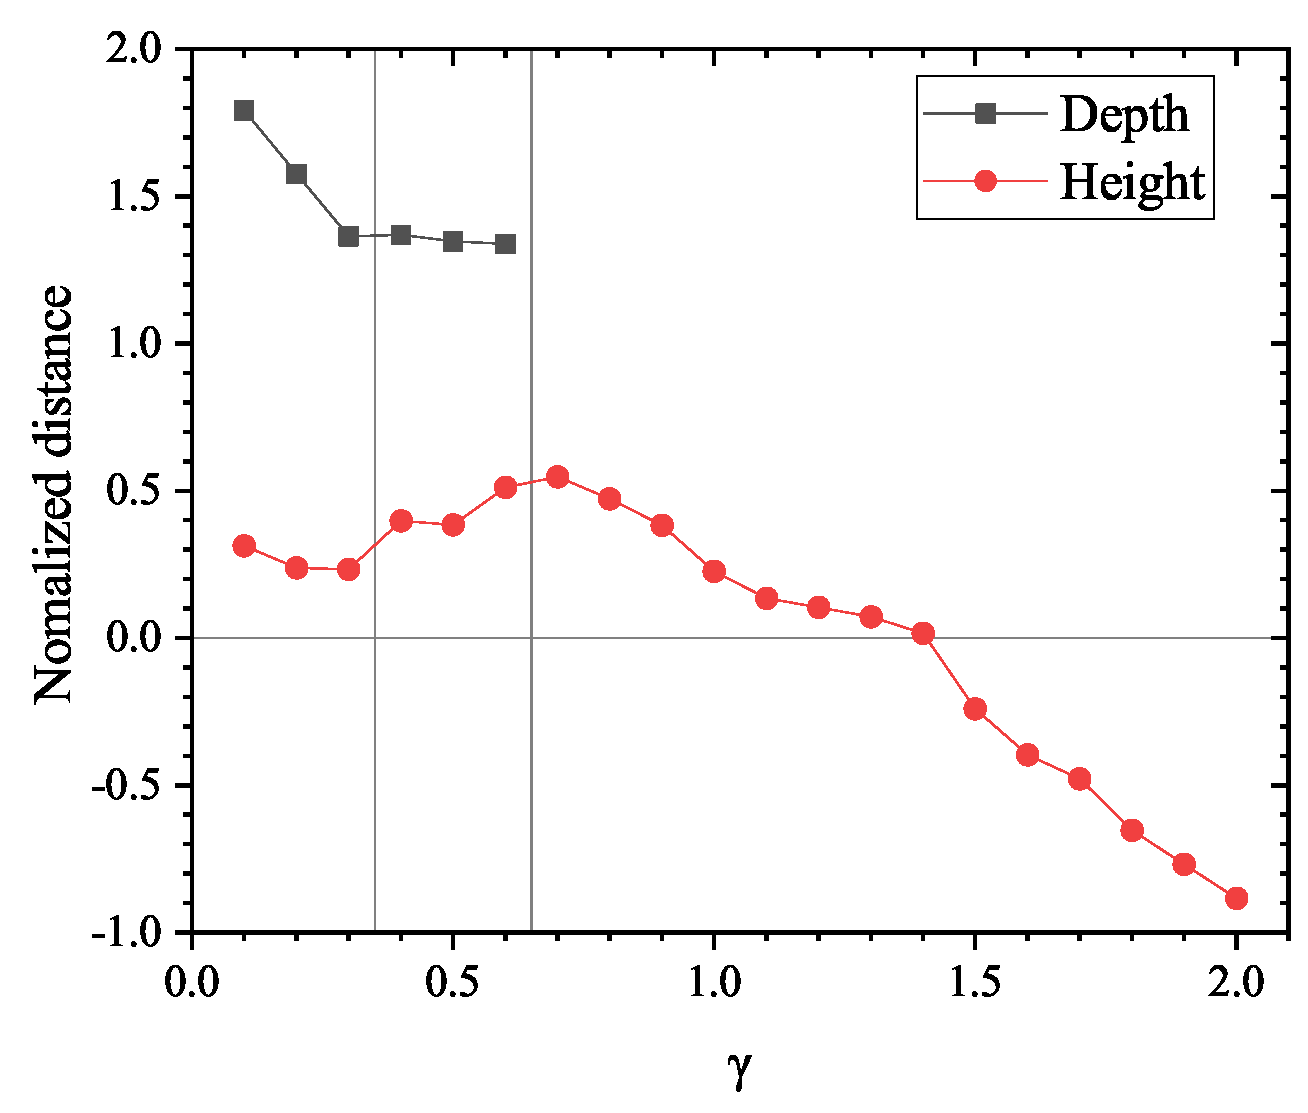
\includegraphics[width=0.6\linewidth]{img/fig3.oildistance.eps}
    \caption{空泡距水-硅油界面不同相对距离情形下的射流深度/高度(双向)}
    \label{fig3.oildistance}
\end{figure}

考虑到水-油界面附近的空泡表现出不同于水气界面的特殊行为,此处重新定义射流深度和高度。以空泡的主体部分的第二次射流撞击界面为节点,在此刻之前,以界面为基准,空泡射流向油侧深入最远的距离为高度,向水侧深入最远的为深度(深度只计断裂式溃灭)。作图\ref{fig3.oildistance}。

从图中可以看到,在$\gamma\geq1.4$时,射流没有到达界面,其高度值为负。但随着$\gamma$的变小,距离界面的距离越來越近。而在$\gamma=1.4$时,空泡的射流能够抵达界面。并且知道$\gamma=0.7$,射流的高度是越来越远的。在射流溃灭机制中,距离壁面越近,射流抵达的高度越高,并且在$\gamma=0.7$时达到最高。而在断裂式溃灭中,在A.断裂接触式($\gamma\leq 0.3$)中,因没有形成射流机制,以其溃灭后的界面最高位置替代。距离界面越近,形成的位置改造越高。而B.断裂射流式($0.4\leq\gamma\leq 0.6$)中,存在射流,但射流头部与二次膨胀的空泡边界无法区分,也以这个无法区分的头部位置为射流高度。其一定程度上符合$\gamma$越大,高度越大。




综合来看空泡在两种软物质界面附近的脉动,在大$\gamma$值的情况下,$\mathbf{\zeta}$具有有效的预言功能。但在小$\gamma$值的情况下,空泡的溃灭形式发生变化,其预言功能失效。

空泡在水气和水油界面结果的不同主要来自其对声传导和粘性的影响。声传导则主要受当地声速和物质密度影响。当地声速可由状态方程获得。高粘性和高密度都增加了空泡的能量耗散,声传导影响空泡的射流形成方式。

\section{单空泡在固体界面附近的脉动}

激光空泡与固体界面的相互作用具有广泛的应用。在实际生产生活中,空泡场景很多的是在固体边界附近,并由此形成独特的动力学特征。在本节中,我们只简单的探讨激光空泡在固定金属壁面的脉动的简化仿真模型——无限大固定壁面附近不同相对间距下的空泡脉动。

\begin{figure}[h]
    \centering
    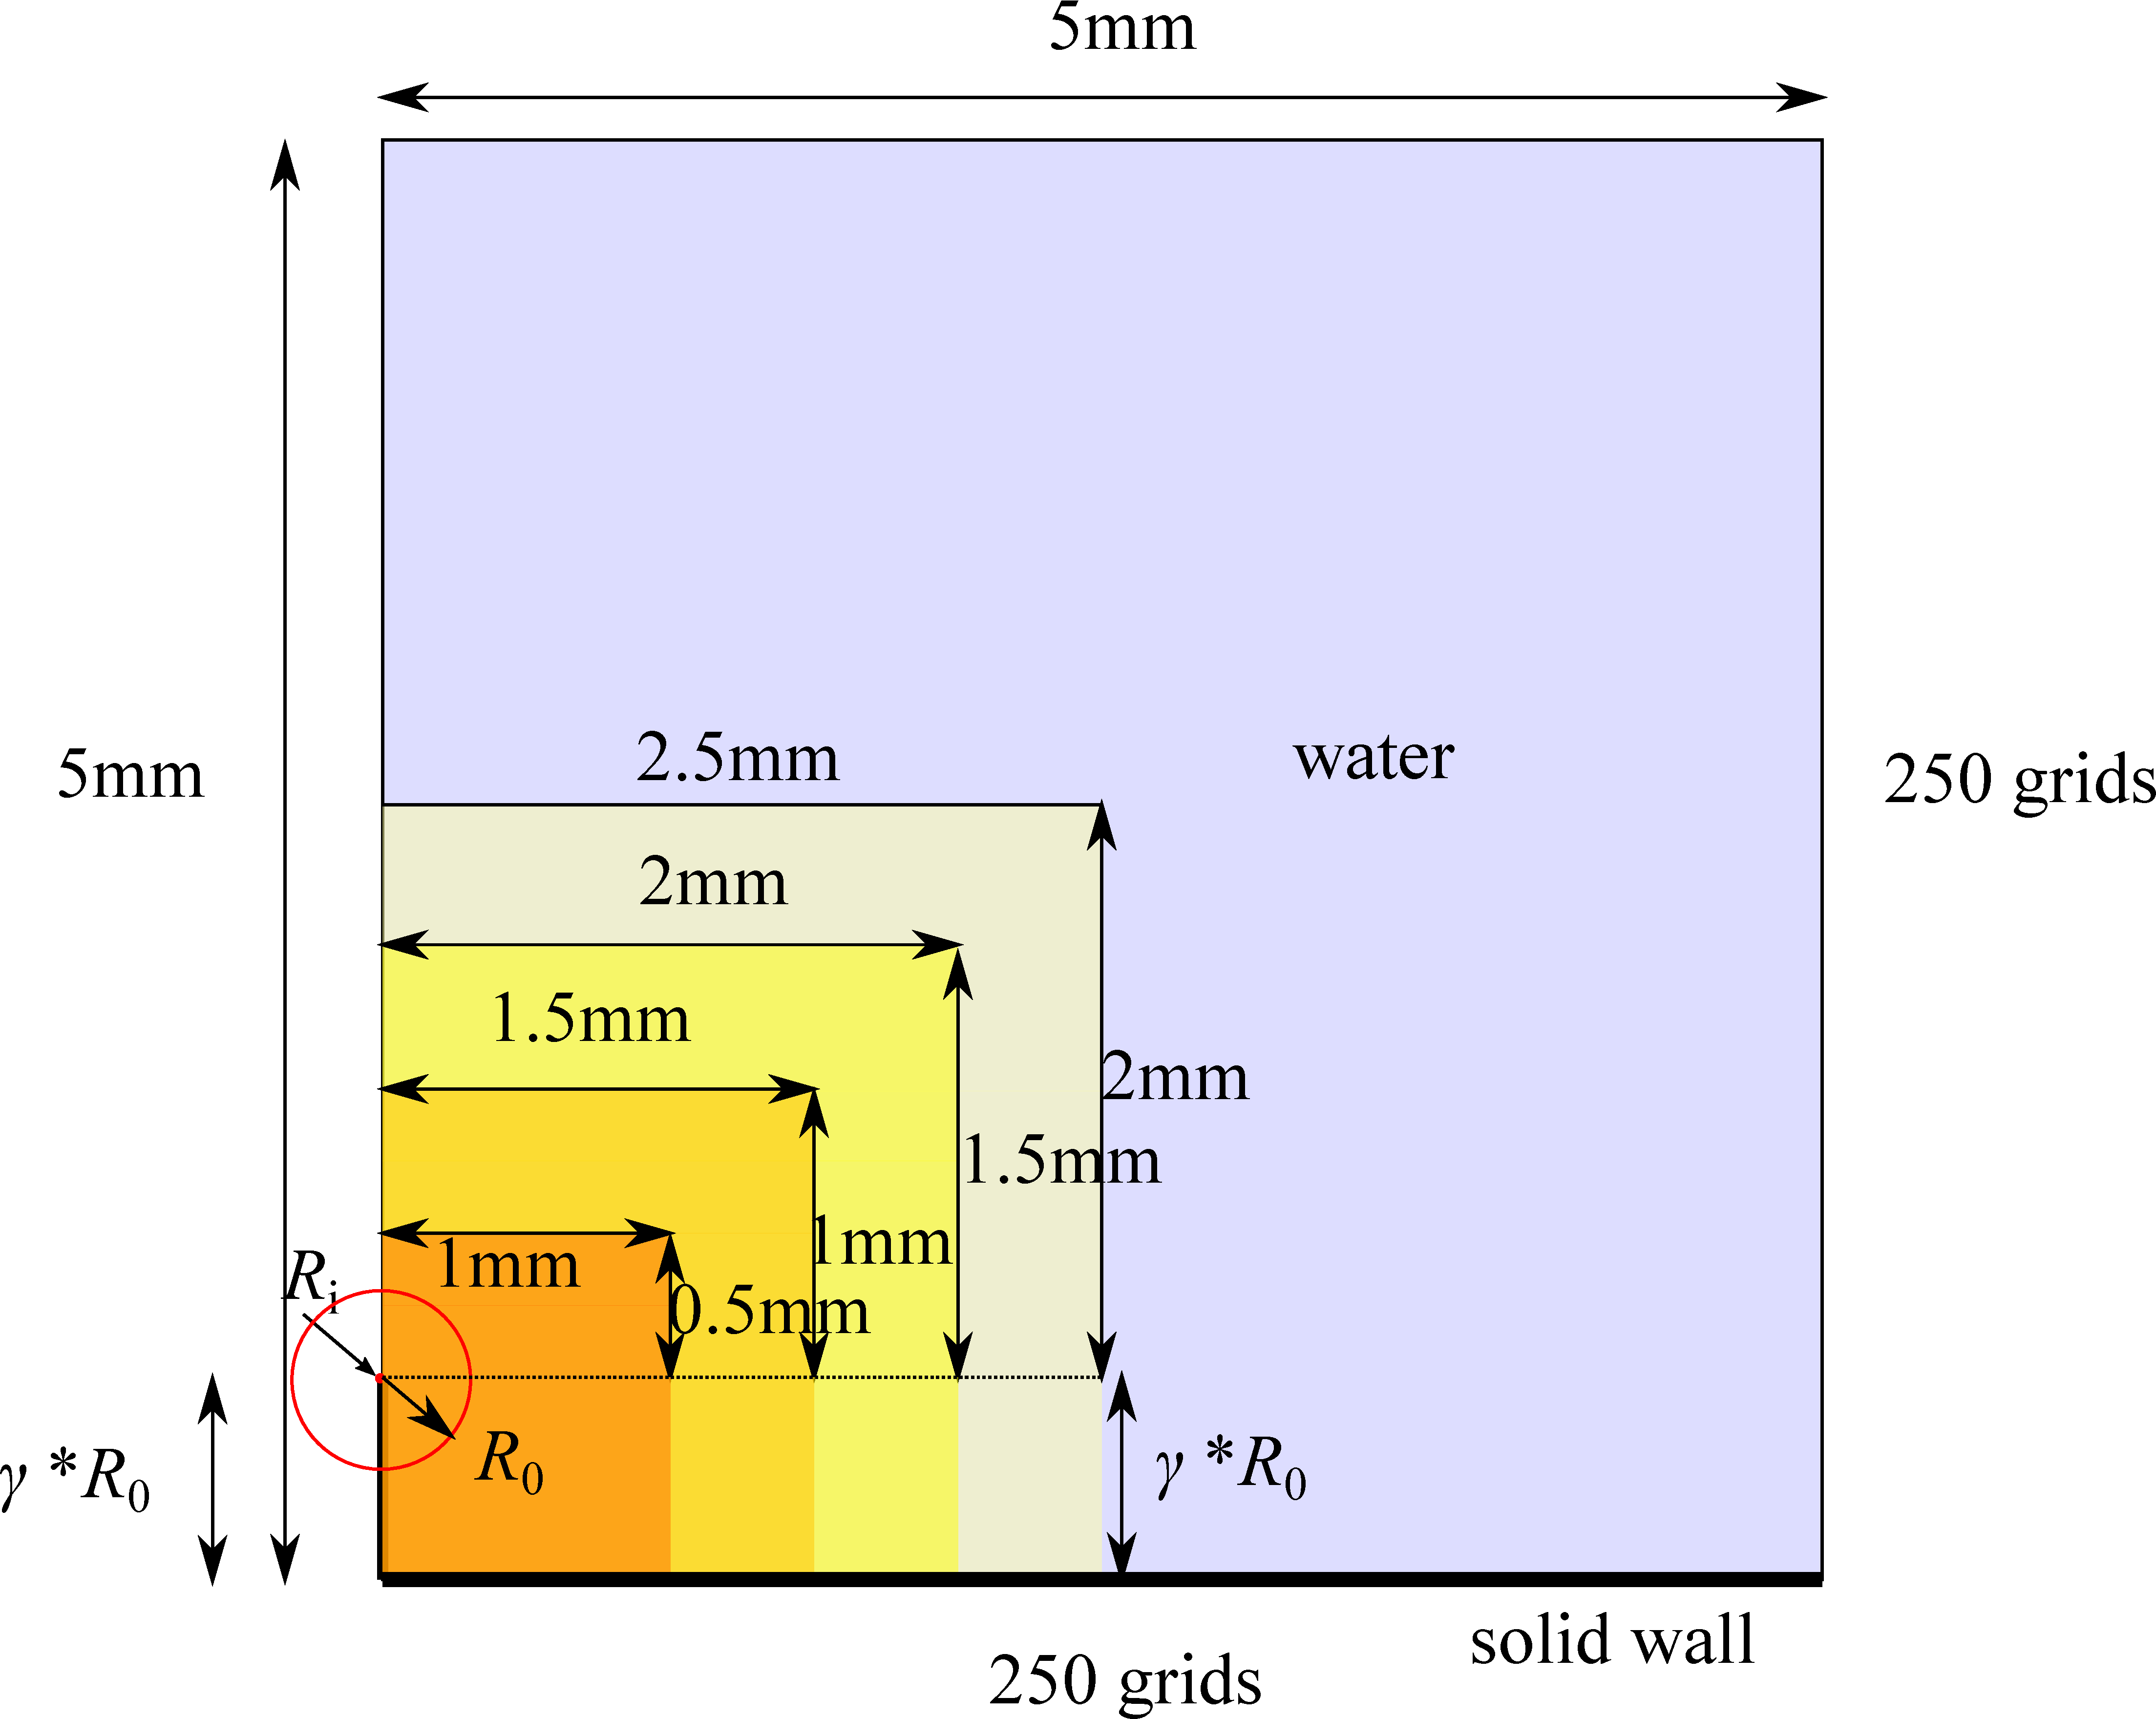
\includegraphics[width=0.7\linewidth]{img/solidwall.pdf}
    \caption{激光致空泡在固体界面附近的脉动计算域设置}
    \label{fig3.solidwallsetup}
\end{figure}

图\ref{fig3.solidwallsetup}显示了计算域的设置。对称轴仍使用对称边界,旋转面使用wedge边界,上边界和右边界都是“wavetransform”的无反射压力边界,和速度“pressureInletOutletVelocity” 流入流出边界。而固体壁面则使用“ZeroGradient”为压力和相边界,以“noSlip”为速度边界。网格密度和加密以及初始空泡设置,与上文中水与软物质界面附近空泡的设置一致。


\begin{figure}[h]
    \centering
    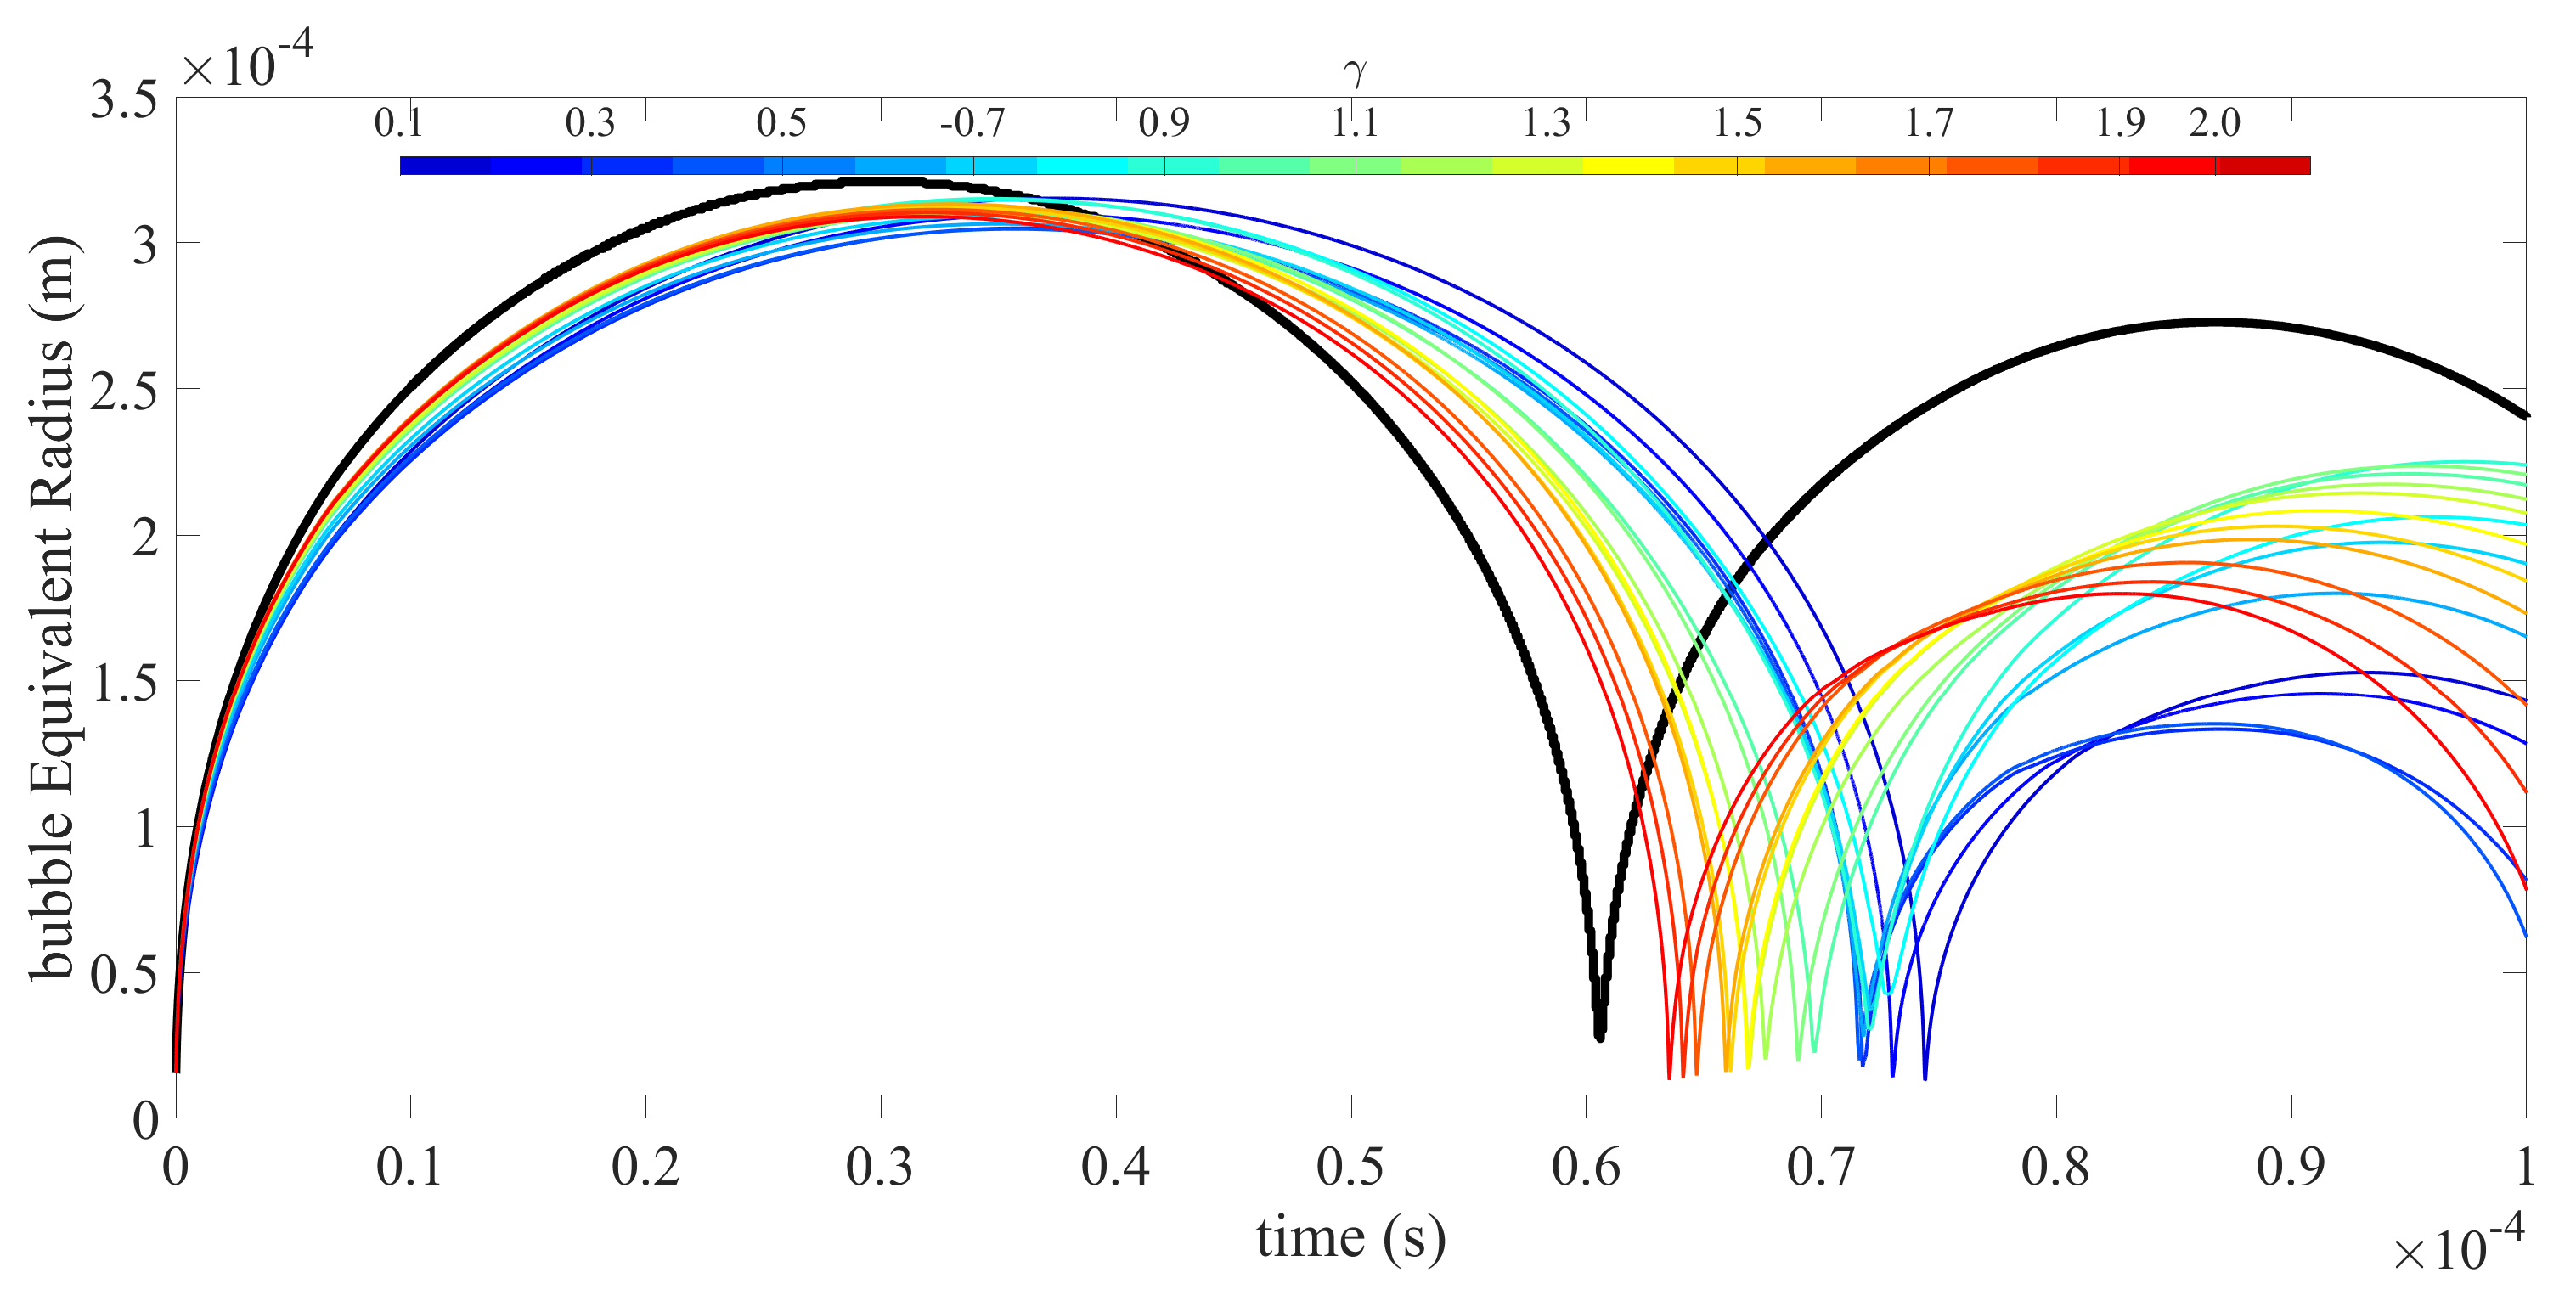
\includegraphics[width=1\linewidth]{img/fig3.solid.eps}
    \caption[空泡距固体界面不同相对距离情形下的泡半径对比图]{空泡距固体界面不同相对距离情形下的泡半径对比图,图中黑色实线为自由域中的模拟结果。}
    \label{fig3.solidradius}
\end{figure}

\begin{figure}[H]
    \centering
    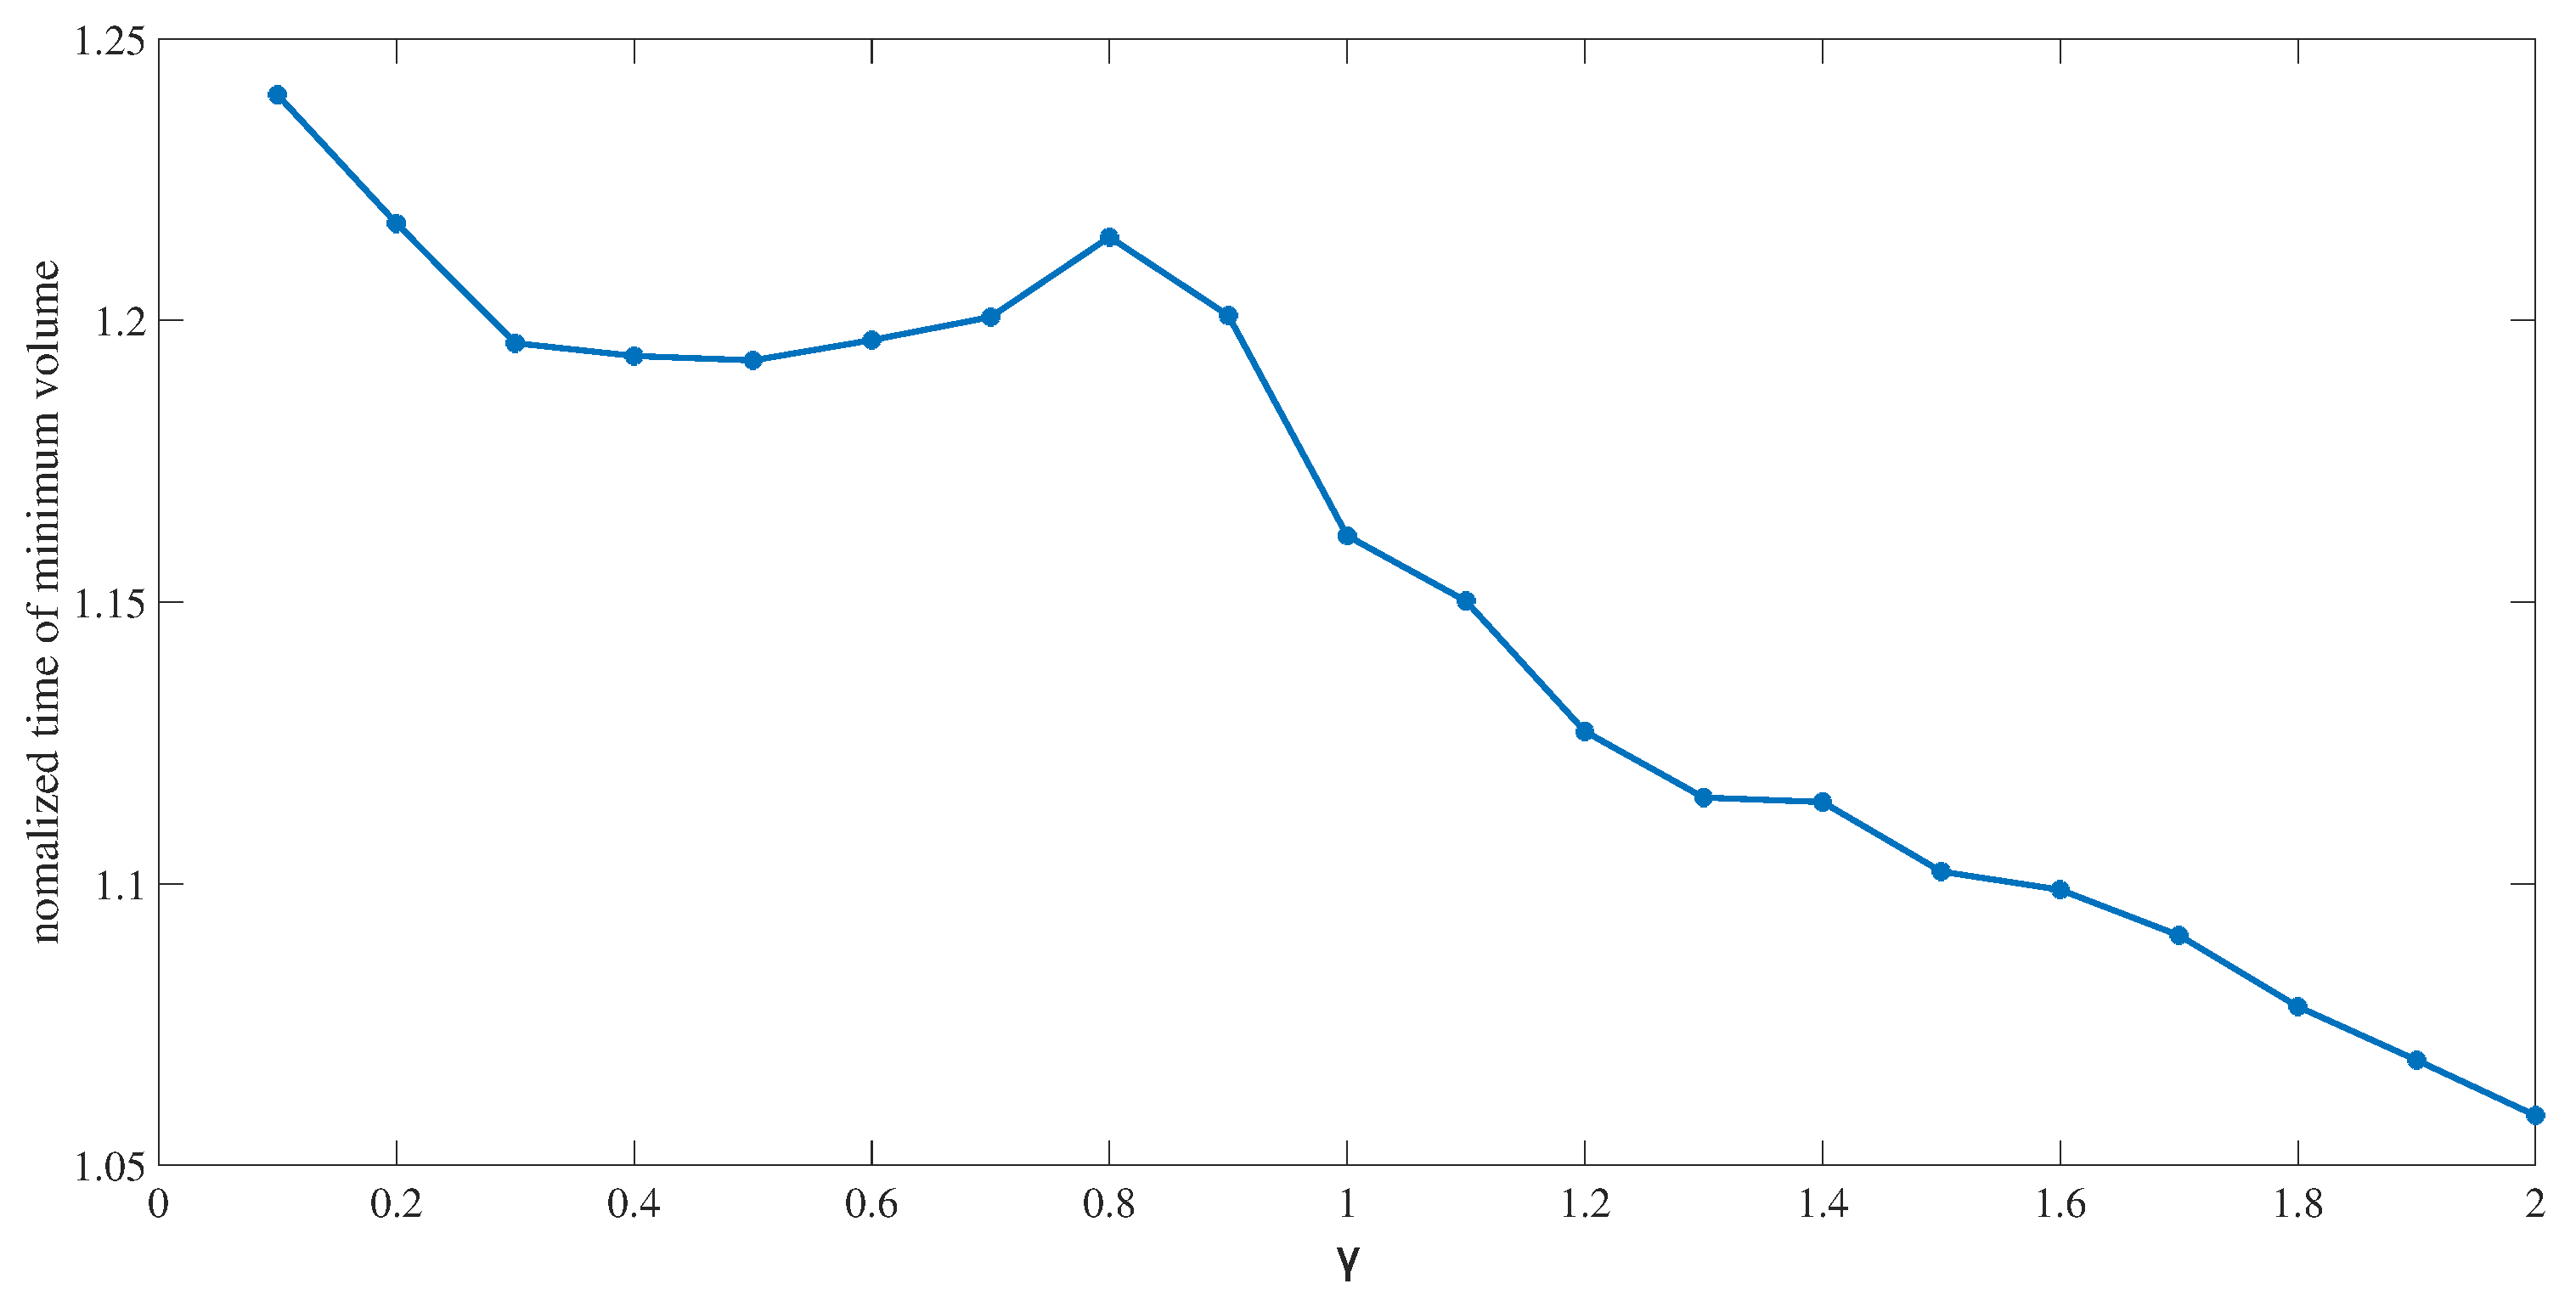
\includegraphics[width=0.9\linewidth]{img/fig3.solidnmlzedcollapsetime.eps}
    \caption[固体壁面附近空泡的归一化溃灭时间]{固体壁面附近空泡的归一化溃灭时间。归一化时间通过模拟计算中获得的体积最小时间除以自由域中的体积最小时间60.06$\mu s $获得。}
    \label{fig3.solidcolltime}
\end{figure}

图\ref{fig3.solidradius}中给出了空泡与固体界面在不同相对距离$\gamma$处的体积等效半径对比图。可以看到,在受固体制约的环境中,空泡的半径并没有达到其在自由域内能达到的高度。同时$\gamma$越大,也就是越接近自由的情况下,空泡的体积等效半径曲线越接近在自由域中的脉动。
在$\gamma\leq 0.2$,也就是空泡在界面附近时,空泡的膨胀曲线相比$\gamma> 0.2$等案例更高跨度更大。该情况可以见图\ref{fig3.solidcolltime}。图中清晰地表示了一个近似随着$\gamma$增大,归一化溃灭时间减少的趋势。这与越远离壁面越接近自由域的现实相符。
特别地,在$0.3\leq \gamma\leq0.8$区间内空泡的归一化体积最小时间有一个上升的趋势。这主要归功于空泡膨胀过程中与壁面接触后,形成粘滞作用。在空泡与壁面接触部分,边界层的存在对空泡的膨胀和收缩进行了一定地延缓。下文中将结合空泡的相-速度-压力云图给出解释。

在图\ref{fig3.solidcolltime}中可以简单的将曲线分为三个阶段,$A\,.$$\gamma\leq 0.2$的久溃灭时间阶段,$B\,. 0.3\leq \gamma\leq0.8$的溃灭时间缓慢增长的阶段,和$C\,.0.9\leq \gamma\leq2.0$的溃灭时间稳步下滑的阶段。在$A\,$阶段,过近的距离使空泡产生特殊的膨胀溃灭机制。其近似半球型的膨胀初期形状将很大的影响空泡的动力学特征。
在$B\,$阶段,因初始距离相对较在$A\,$阶段有明显的增大,从而在膨胀时虽然与壁面接触,但空泡也将受到壁面形成的推动作用。在这个阶段,空泡与壁面接触的时长也随着$\gamma$增长而减小,由此也表现出他独立的动力学特征。
在$C\,$阶段,空泡形成“常规的”射流动态,也就是空泡膨胀和溃灭都没有接触壁面,但受壁面影响形成压力梯度,从而形成射流。

下文将针对$A\,$,$B\,$,$C\,$三个阶段,各自选取一个案例对该种情况进行更细致的解释。其中$A\,$阶段,选取$\gamma=0.1$;$B\,$阶段,选取$\gamma=0.7$;在$C\,$阶段,选取$\gamma=2.0$。
%$0.3\leq \gamma\leq0.8$这个阶段主要是因为与壁面接触的时间越來越短而受到的限制作用逐渐减小。


\begin{figure}[h]
    \centering
    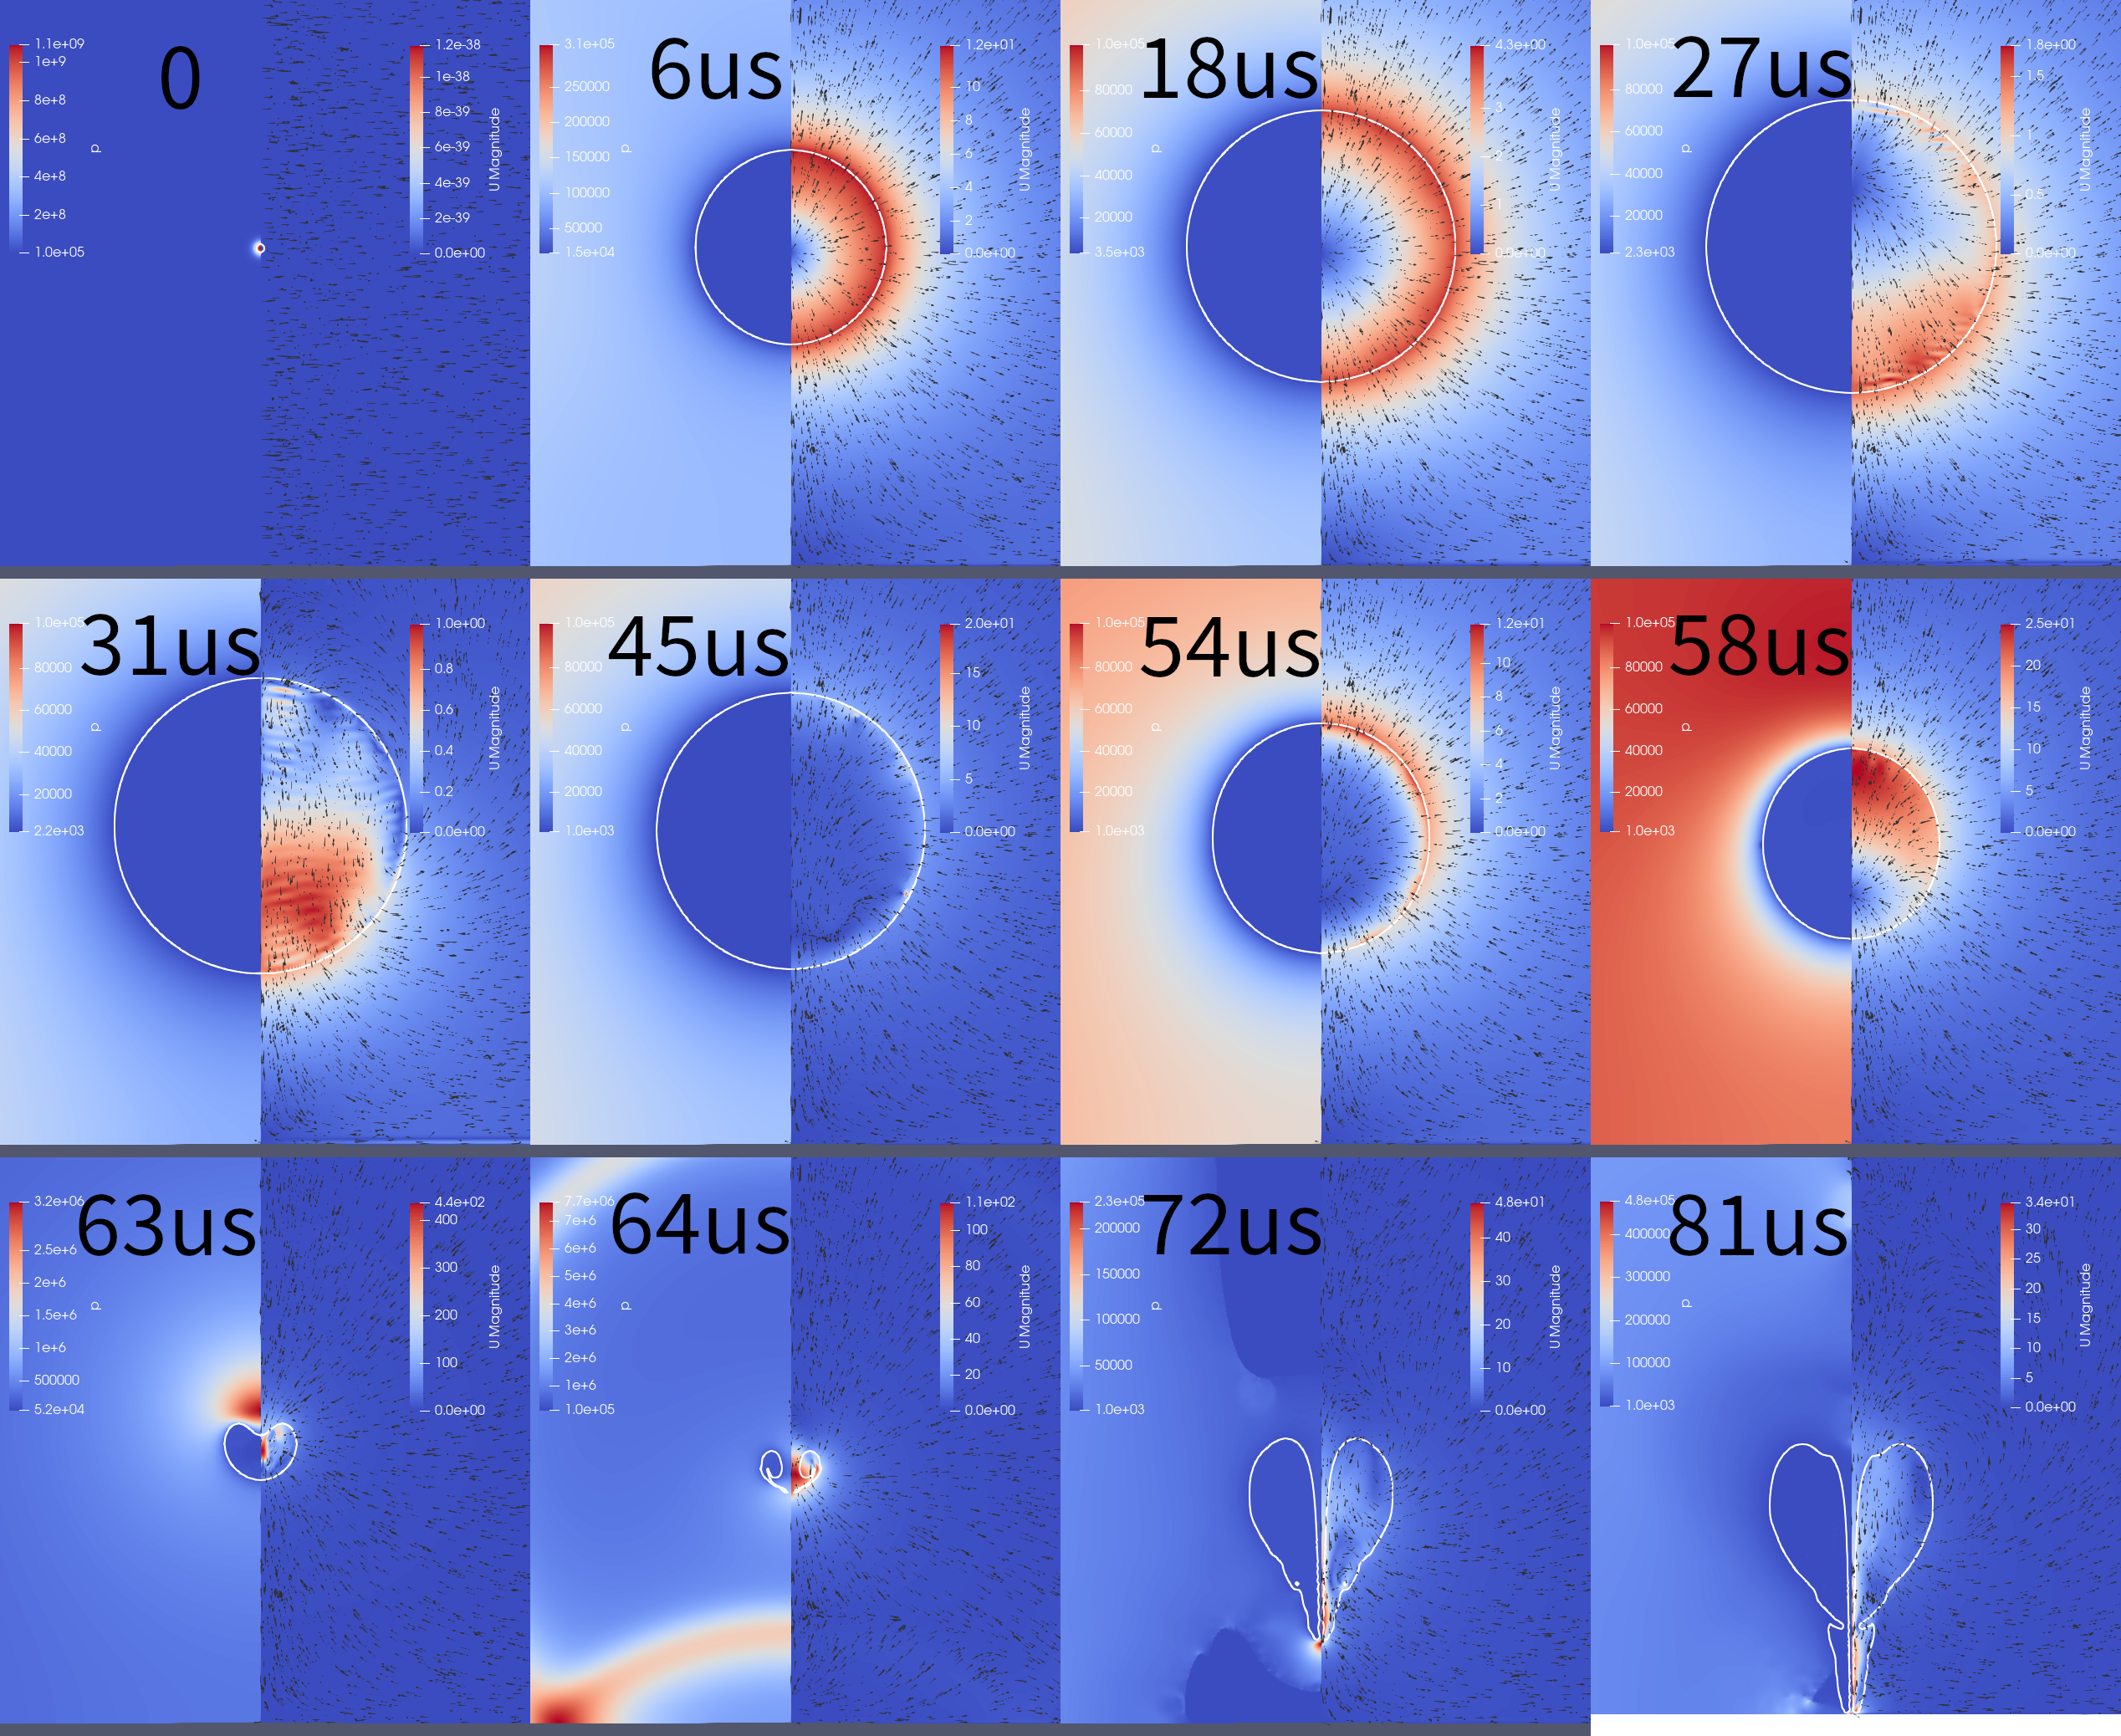
\includegraphics[width=0.9\linewidth]{img/solid2.0.png}
    \caption{空泡距固体界面$\gamma=2.0$情形下的相-速度-压力云图。}
    \label{fig3.gamma2}
\end{figure}
图\ref{fig3.gamma2}显示了$\gamma=2.0$时,空泡的相(白线表示空泡表面)-速度(右半部分图+箭头指示方向)-压力云图(左半部分)。从该图的第一栏可以看到,空泡在膨胀初期,如同自由域孤立单空泡一样各向同的膨胀。并逐渐释放泡内高压至水的饱和蒸汽压附近。在第三帧(18$\mu s$)中可以看到,空泡下部外缘形成较上部更宽的低压带。这个低压带在下一帧(27$\mu s$)中促使空泡向下移动,形成低速度区域的上移。

在第二栏的第一帧(31$\mu s$)中,空泡膨胀到最大泡半径。此时,低压带仍然存在,且速度矢量已经形成自上而下的趋势。可以看到,在空泡内部,速度指向为从上到下的。而在空泡外部上半部(北极),形成环流流向空泡上方。在空泡的下半部,速度指向壁面,并受壁面阻挡,而形成横向的外流。这时,空泡虽然处于最大泡半径时期,但已经形成了溃灭射流的潜在成因。在第二帧(45$\mu s$)中,空泡处于收缩状态。此时可见到空泡内部的下半部形成一个速度矢量的终点区域。这表明,空泡已经形成不均匀的收缩。在下一帧(54$\mu s$)中,空泡持续收缩,壁面速度继续提高。在第四帧(58$\mu s$)中,已经明显可见的形成了压力梯度,和速度梯度。就是空泡的外部的上半部分形成高压,而下半部分仍保持较低的压力。空泡内部的上半部分的速度继续提高,与下半部形成数量级的差别。此时,射流形成。

在第三栏中,第一帧(63$\mu s$)显示了空泡击穿前的流场。此时因空泡的持续收缩,水从上方持续的流向空泡上方,在空泡的上方形成一个高压区,这个高压区直接的驱动了射流的加速射向空泡低面。此时空泡内气体的流速达到440m/s。在第二帧(64$\mu s$)中,射流击穿空泡,空泡形成独特的花托(torus)状。在击穿过程中,因水体的碰撞形成巨大的能量释放,在碰撞过程中,向外辐射了一个冲击波。其在水中传播和反射,形成一个声速压力波。在第三帧(72$\mu s$)中,射流沿着对称轴方向继续前进。并在第四帧(81$\mu s$)中,射流撞击到固壁面。而此时射流的速度已经衰减到30m/s的量级。

在这个案例中,空泡形成“常规的”射流。就是在射流形成过程中,自空泡的北极先发生平化,继而向空泡内凹陷,然后发展成尖端点射流,除端点外边界拓扑没有形成突变,在射流击穿空泡后,继续前进了一段距离。这种“常规的”射流,有时发生在溃灭后期,有时发生在空泡回弹阶段。


\begin{figure}[h]
    \centering
    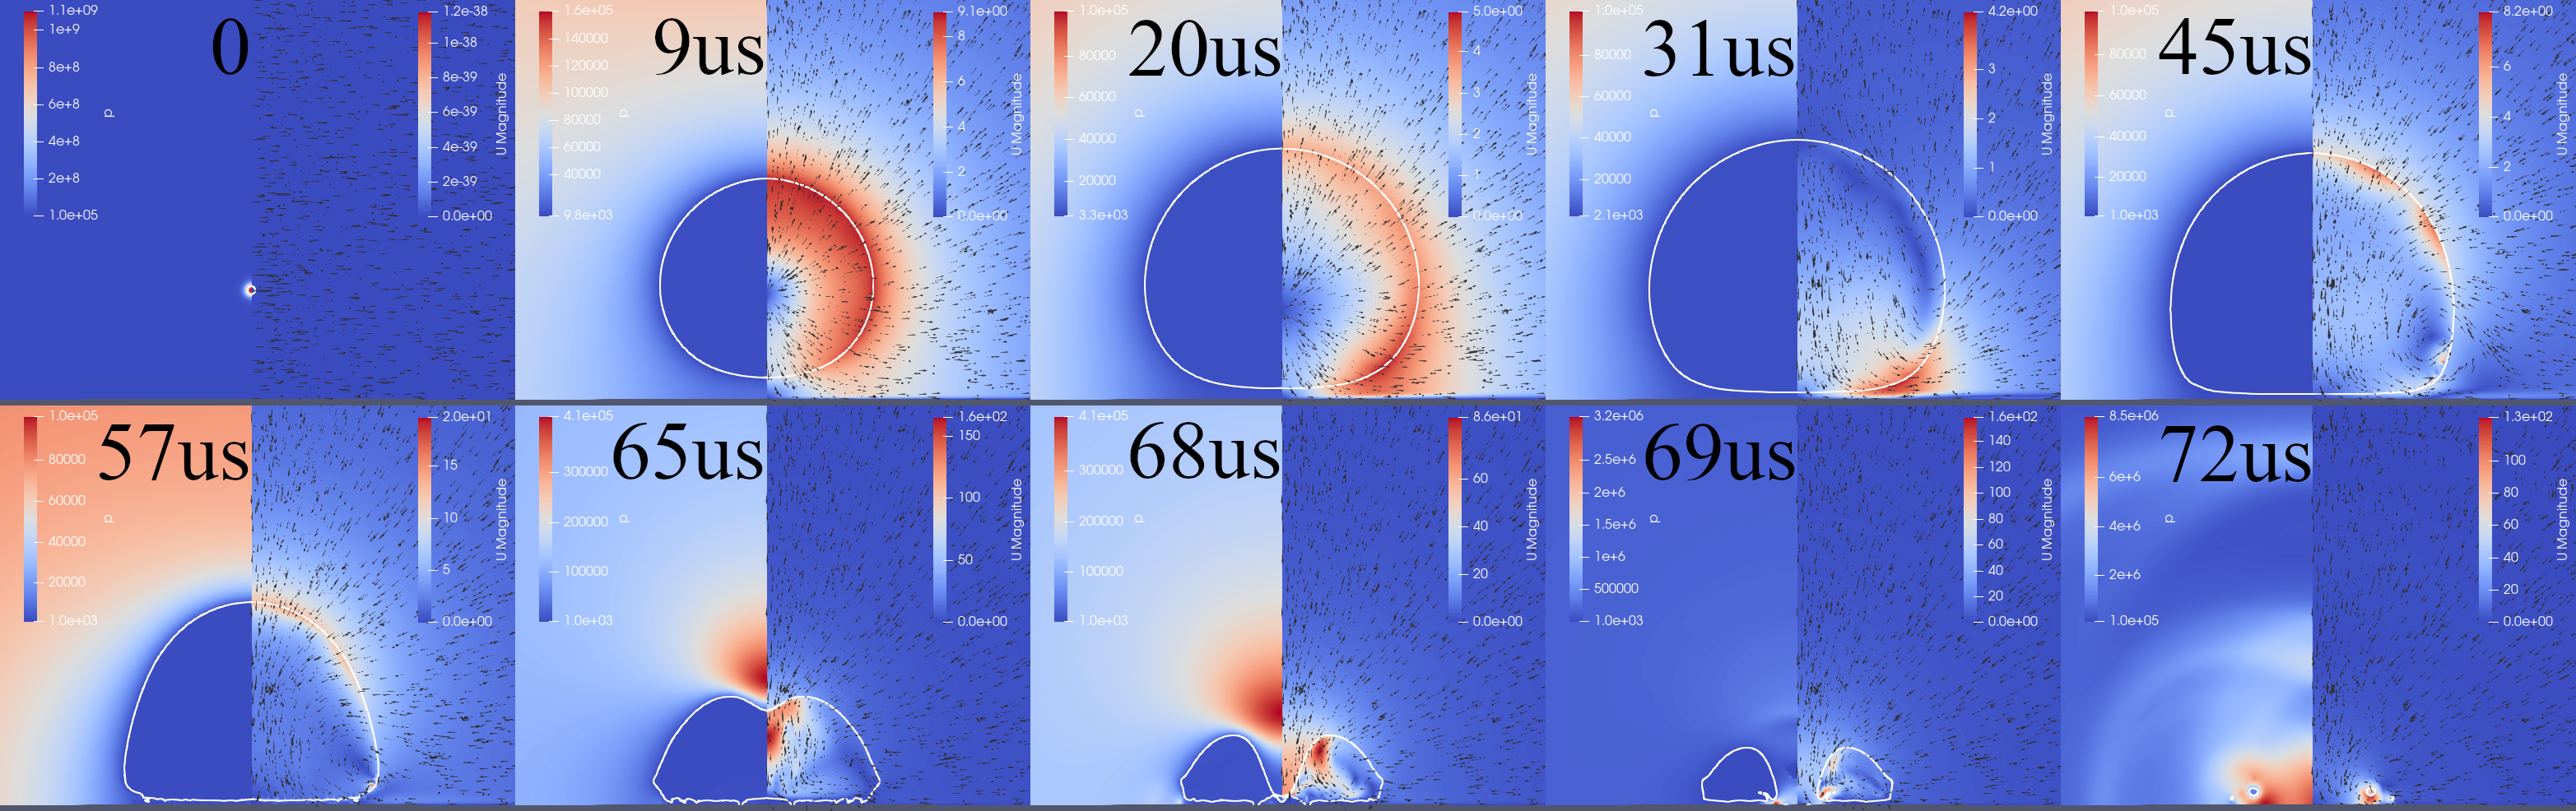
\includegraphics[width=0.9\linewidth]{img/3.solid0.7.png}
    \caption{空泡距固体界面$\gamma=0.7$情形下的相-速度-压力云图}
    \label{fig3.gamma0.7}
\end{figure}

图\ref{fig3.gamma0.7}展示了$\gamma=0.7$时,空泡的相(白线表示空泡表面)-速度(右半部分图+箭头指示方向)-压力云图(左半部分)。从第二帧($9\mu s$)中可以看到,空泡在膨胀初期就形成了膨胀的各向分化。在冲击波反射后,空泡的下方形成低压区,而空泡的上方则形成相对高压。但同时因固壁面的限制,空泡的下半部分(南极)出现平化,以及粘滞效应造成的低速度区。空泡的上半部分的膨胀速度远超下半部分,。同时因为压力的释放,在空泡的初始位置区域产生低速度区。空泡下半部分的外流场形成平行于壁面的发散流。第三帧($20\mu s$)空泡继续膨胀,但因为空泡的上半部分持续膨胀,内外压差降低并逐渐平滑,其速度逐渐下降。而同时,因固壁面的粘滞作用,空泡下半部分没有发生平化的区域,也就是没有直接面对壁面的区域速度没有发生较大变化。从而空泡的形状向帽子型逐渐演化。第四帧($31\mu s$)中,空泡达到最大泡半径。从速度图中可以看到一条蓝色带,其作为速度矢量的初始位置。这说明当前帧空泡外部的水惯性的外流,但空泡内部已经形成自上而下的速度趋势,此时异方向的速度值差别不大,均在1m/s左右。但可以看到,空泡南极的向外延展部分仍处于较高速度。即空泡下部仍保持膨胀状态。这是由于底部仍存在压差空间、壁面粘滞和惯性的共同作用。第五帧($45\mu s$)中,空泡南极的延展部分彻底平化,这是上一帧相对高速运动的结果。但同时,除这个延展接驳处仍作为速度矢量的终点方向外,因内外压差的驱动,全流场形成指向空泡的速度。空泡内部也形成自上而下的速度趋势。并在空泡下半部分转而指向上述接驳处。

在第二栏第一帧($57\mu s$)中,因全流场的运动的推动,空泡持续收缩。因北极附近形成更高的压力梯度,其速度逐渐开始提高。并且因空泡内部低压低密度气体也同时向壁面运动,空泡底部与壁面贴合得更加紧密。这也使空泡南极与壁面的接合部分成为全流场的速度终点。同样地,可以看到上文中的接驳处形成特殊的蘑菇伞盖状边缘结构。这种结构的底部是受固壁面的粘滞导致的收缩缓慢,以及当地作为空泡内部的速度出口影响而形成的。在下一帧中($65\mu s$),空泡北极附近因水的汇集而产生约4bar的高压。这个高压将驱动水射流的产生和射向空泡内部以及壁面。空泡内部也因水的持续汇集而形成高速的指向壁面的速度。值得注意的是,此时所谓的蘑菇状结构仍然存在,并将继续存在到溃灭。在第三帧($68\mu s$)中,射流在外界4.1bar的压力驱动下,撞击到空泡的南极。而蘑菇状特殊结构仍然存在,但有所收缩。下一个微秒($69\mu s$),因射流撞击壁面产生Blake Splash\cite{blake_art_1997, blake_acoustic_1999}(巴拉克喷溅)。在最后一帧($72\mu s$)中,空泡因喷溅和微射流而分裂,分裂后的每一部分单独溃灭时,都向外辐射了冲击波,并对隔壁空泡的溃灭进行了溃灭加强,形成较强的空泡南极位置的高压加强和多轮冲击波辐射。

在本例的这种情况下,空泡膨胀并与壁面发生贴合和黏连,导致空泡与壁面的接触面在水平方向上的膨胀时间较长,收缩速度较慢,形成特殊的溃灭结构。射流在击穿空泡下表面的几乎同时也到达壁面。在这种情况中,$\gamma$越大,接触面相对较小,但共同有类似的动力学过程。


\begin{figure}[h]
    \centering
    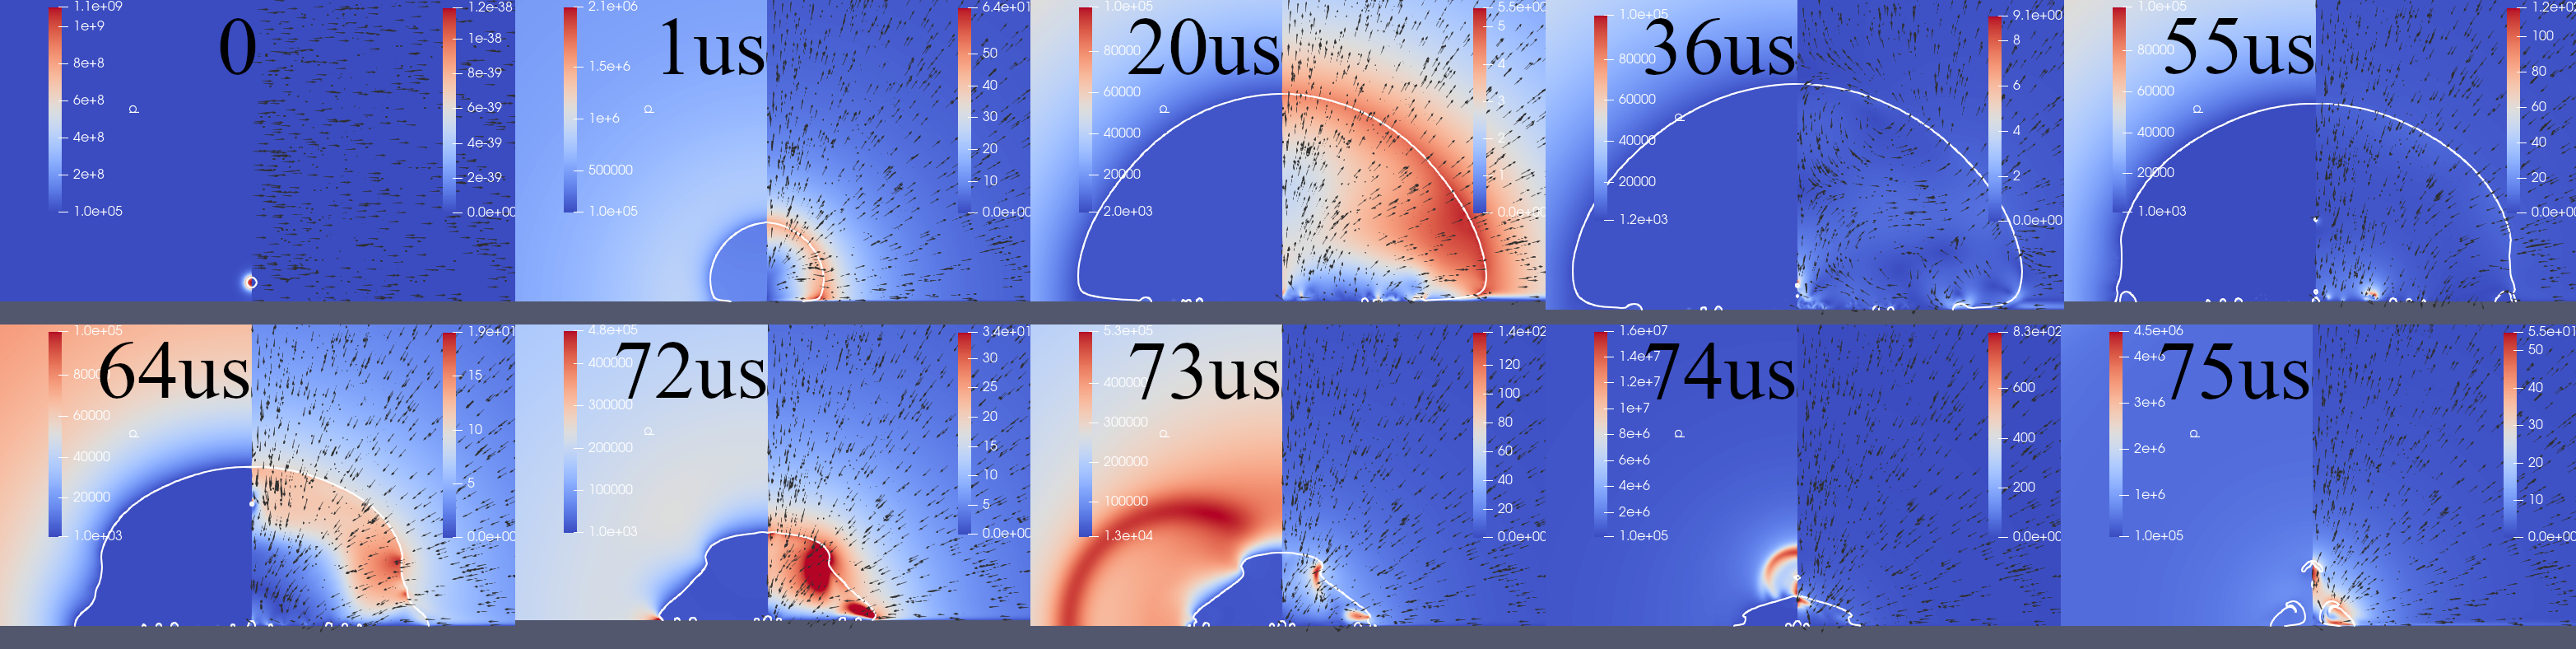
\includegraphics[width=0.9\linewidth]{img/3.solid0.1.png}
    \caption{空泡距固体界面$\gamma=0.1$情形下的相-速度-压力云图}
    \label{fig3.gamma0.1}
\end{figure}

图\ref{fig3.gamma0.1}展示了$\gamma=0.1$时,空泡的相(白线表示空泡表面)-速度(右半部分图+箭头指示方向)-压力云图(左半部分)。也是最为特殊的一种情况。
在首栏第一帧显示了空泡的初始位置,这时空泡几乎贴近固壁面。于是产生了在第二帧($ 1\mu s$)中,空泡形成的半球外型。此时,空泡的下表面贴合固壁面表面。而在边缘接驳处贴合位置尚未移动达到此处,其形成水膜层。此时就形成上文中特殊的蘑菇型结构。可以注意到,此时的速度在$Y>\gamma \times R_0$以上位置是呈扇形散射的。而在$Y<\gamma \times R_0$形成一个平行与壁面的流动。在空泡初始位置以下接近上述接驳处的空泡表面具有相对最高的速度。这是由于空泡初始能量的点源释放时,近固壁面方向受阻挡,物质在此处集中释放。于是形成下一帧($20\mu s$)中,此处的空泡界面追赶上其他方向的位置,形成半球型。但同时因固壁面的粘滞作用,这个接驳点仍然存在。空泡壁面此时仍受惯性驱动而继续向膨胀。而速度的集中释放位置也因固壁面粘滞的限制而上移到远离壁面的位置。在第四帧($36\mu s$)中,空泡到达其最大泡半径位置。此时空泡内外的速度都极小,将在下一时刻因外部高压的驱动而形成向内的速度。值得注意的是,上述的接驳处相比前一帧形成更加垂直的趋势。
第五帧($55\mu s$)显示了空泡收缩时的一个状态。靠近壁面的水平流推动空泡的下部垂直的移动,而空泡的上部则受辐射状汇聚的水流推动,形成扁帽式收缩。于是在水平流和辐射流的相交位置产生一种下部内嵌进上部的连接结构,有时也成为扭结结构。这种结构的早期诞生为后续现象的诞生确定最关键的因素。

第二栏中显示了空泡溃灭的一个序列。第一帧($64 \mu s$)中,近壁面的水平流持续推进壁面向对称轴运动。但壁面的粘滞作用使空泡贴在壁面部分很少的移动,也是靠近底部的部分对水平流的推动反应不明显。水平流的推动以及其被粘滞层挤压向上的移动和辐射流的推动,是内嵌结构处产生速度的叠加,形成高速点。这种速度的叠加在嵌入结构处持续演化,在第二帧($ 72\mu s$)中,其局部速度达到30m/s,较上一帧几乎翻倍。在本帧中,空泡壁面在水平流的推动和壁面粘滞的作用下,在空泡下部形成较大的倾斜度,同时在上方向下压迫的辐射流也对这个现象有贡献。另外值得注意的一点是,在空泡与壁面连接的地方,因当地存在连续的几个水滴。在泡外水体接触到这几个水滴后,立刻成为泡外水体的一部分。使空泡下边缘再次产生上文中特殊的蘑菇伞盖结构。此处蘑菇结构为在下一帧($ 73\mu s$)中表现出的冲击波负主要责任。而在此帧中,流域内的水持续想低压去域移动,内嵌结构处的收缩速度已经达到140m/s,与其他部位的40m/s产生较大的差距。随后在下一帧($ 74\mu s$)中,内嵌结构收缩撞击产生一个冲击波,这个冲击波在传播衰减后仍达到了160bar以上。而内嵌结构以上的空泡上部随结构的撞击而脱离空泡本体,形成一个微气泡。而在内嵌式结构撞击后,形成一个高速的朝向上下两个方向的射流,但因为上部本就是水体环境,只表现为高压局部。而空泡内则形成一个针状射流,其速度可以达到近1000m/s,在图中表现为衰减后的830m/s。同样的现象,Fabian和C-D,Ohl实验发现并解释了该现象\cite{reuter_supersonic_2021},如图\ref{fig3.needlejet}所显示的。在图\ref{fig3.gamma0.1}最后一帧中,射向空泡的射流击穿空泡,撞击壁面,沿着壁面方向延展,并发射了一个冲击波(传播出视野)。而被嵌入式结构截断的微空泡在向上方向的射流推动下继续向上运动及回弹。


\begin{figure}[h]
    \centering
    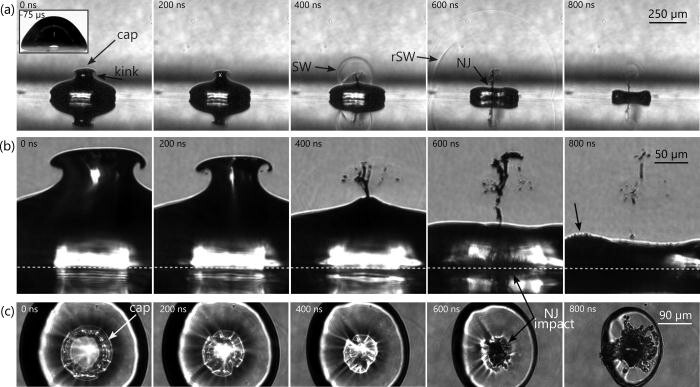
\includegraphics[width=0.9\linewidth]{img/fig3fabiandieter.jpg}
    \caption[实验发现的内嵌式结构和针状射流]{实验发现的内嵌式结构和针状射流\cite{reuter_supersonic_2021}。}
    \label{fig3.needlejet}
\end{figure}

在这种情况下,空泡形成一个半球型,其不是简单的形成一个自上而下的射流,而是形成特殊的内嵌式结构,空泡的这个结构在左右方向上持续收缩,最后撞击产生高压并形成向下的超高速射流。在这之前,空泡一直没有形成射流初始状态的内凹。



\begin{figure}[h]
    \centering
    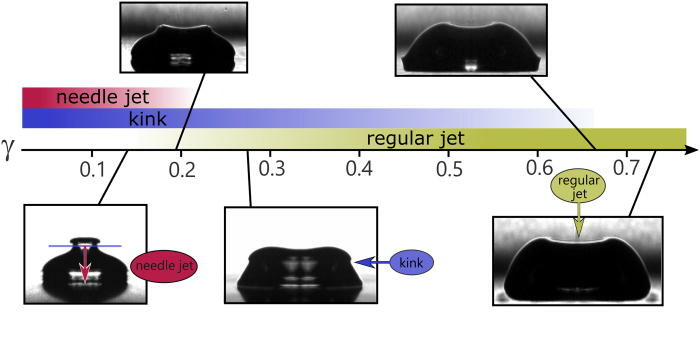
\includegraphics[width=0.7\linewidth]{img/figkink.jpeg}
    \caption[实验发现的内嵌式结构和射流的分野]{Fabian 和CD, Ohl实验发现的内嵌式结构和射流的分野\cite{reuter_supersonic_2021}。}
    \label{figkink}
\end{figure}



%$\gamma$ 对脉动形式的影响
空泡在距离壁面不同$\gamma$ 时表现出不同动力学特征。当$0.9\leq \gamma\leq2$(本文中所做案例的上限)时, 射流在击穿空泡后射向壁面,且空泡在射流击穿前其下半部分保持较好的球性。当$\gamma=\{0.3,0.4,0.5,0.6,0.7,0.8,\}$ 时,空泡粘着在壁面上,并形成特殊的空泡结构。射流在形成后指向壁面,并促使射流击穿空泡的同时也接触壁面,从而形成BlakeSplash。$\gamma=\{0.1,0.2\}$时,空泡形成一种嵌入时结构,这种嵌入式结构在收缩时碰撞并随之形成高速针样射流。
这与实验结果\ref{figkink}\cite{reuter_supersonic_2021}的结果一致。


\begin{figure}[h]
    \centering
    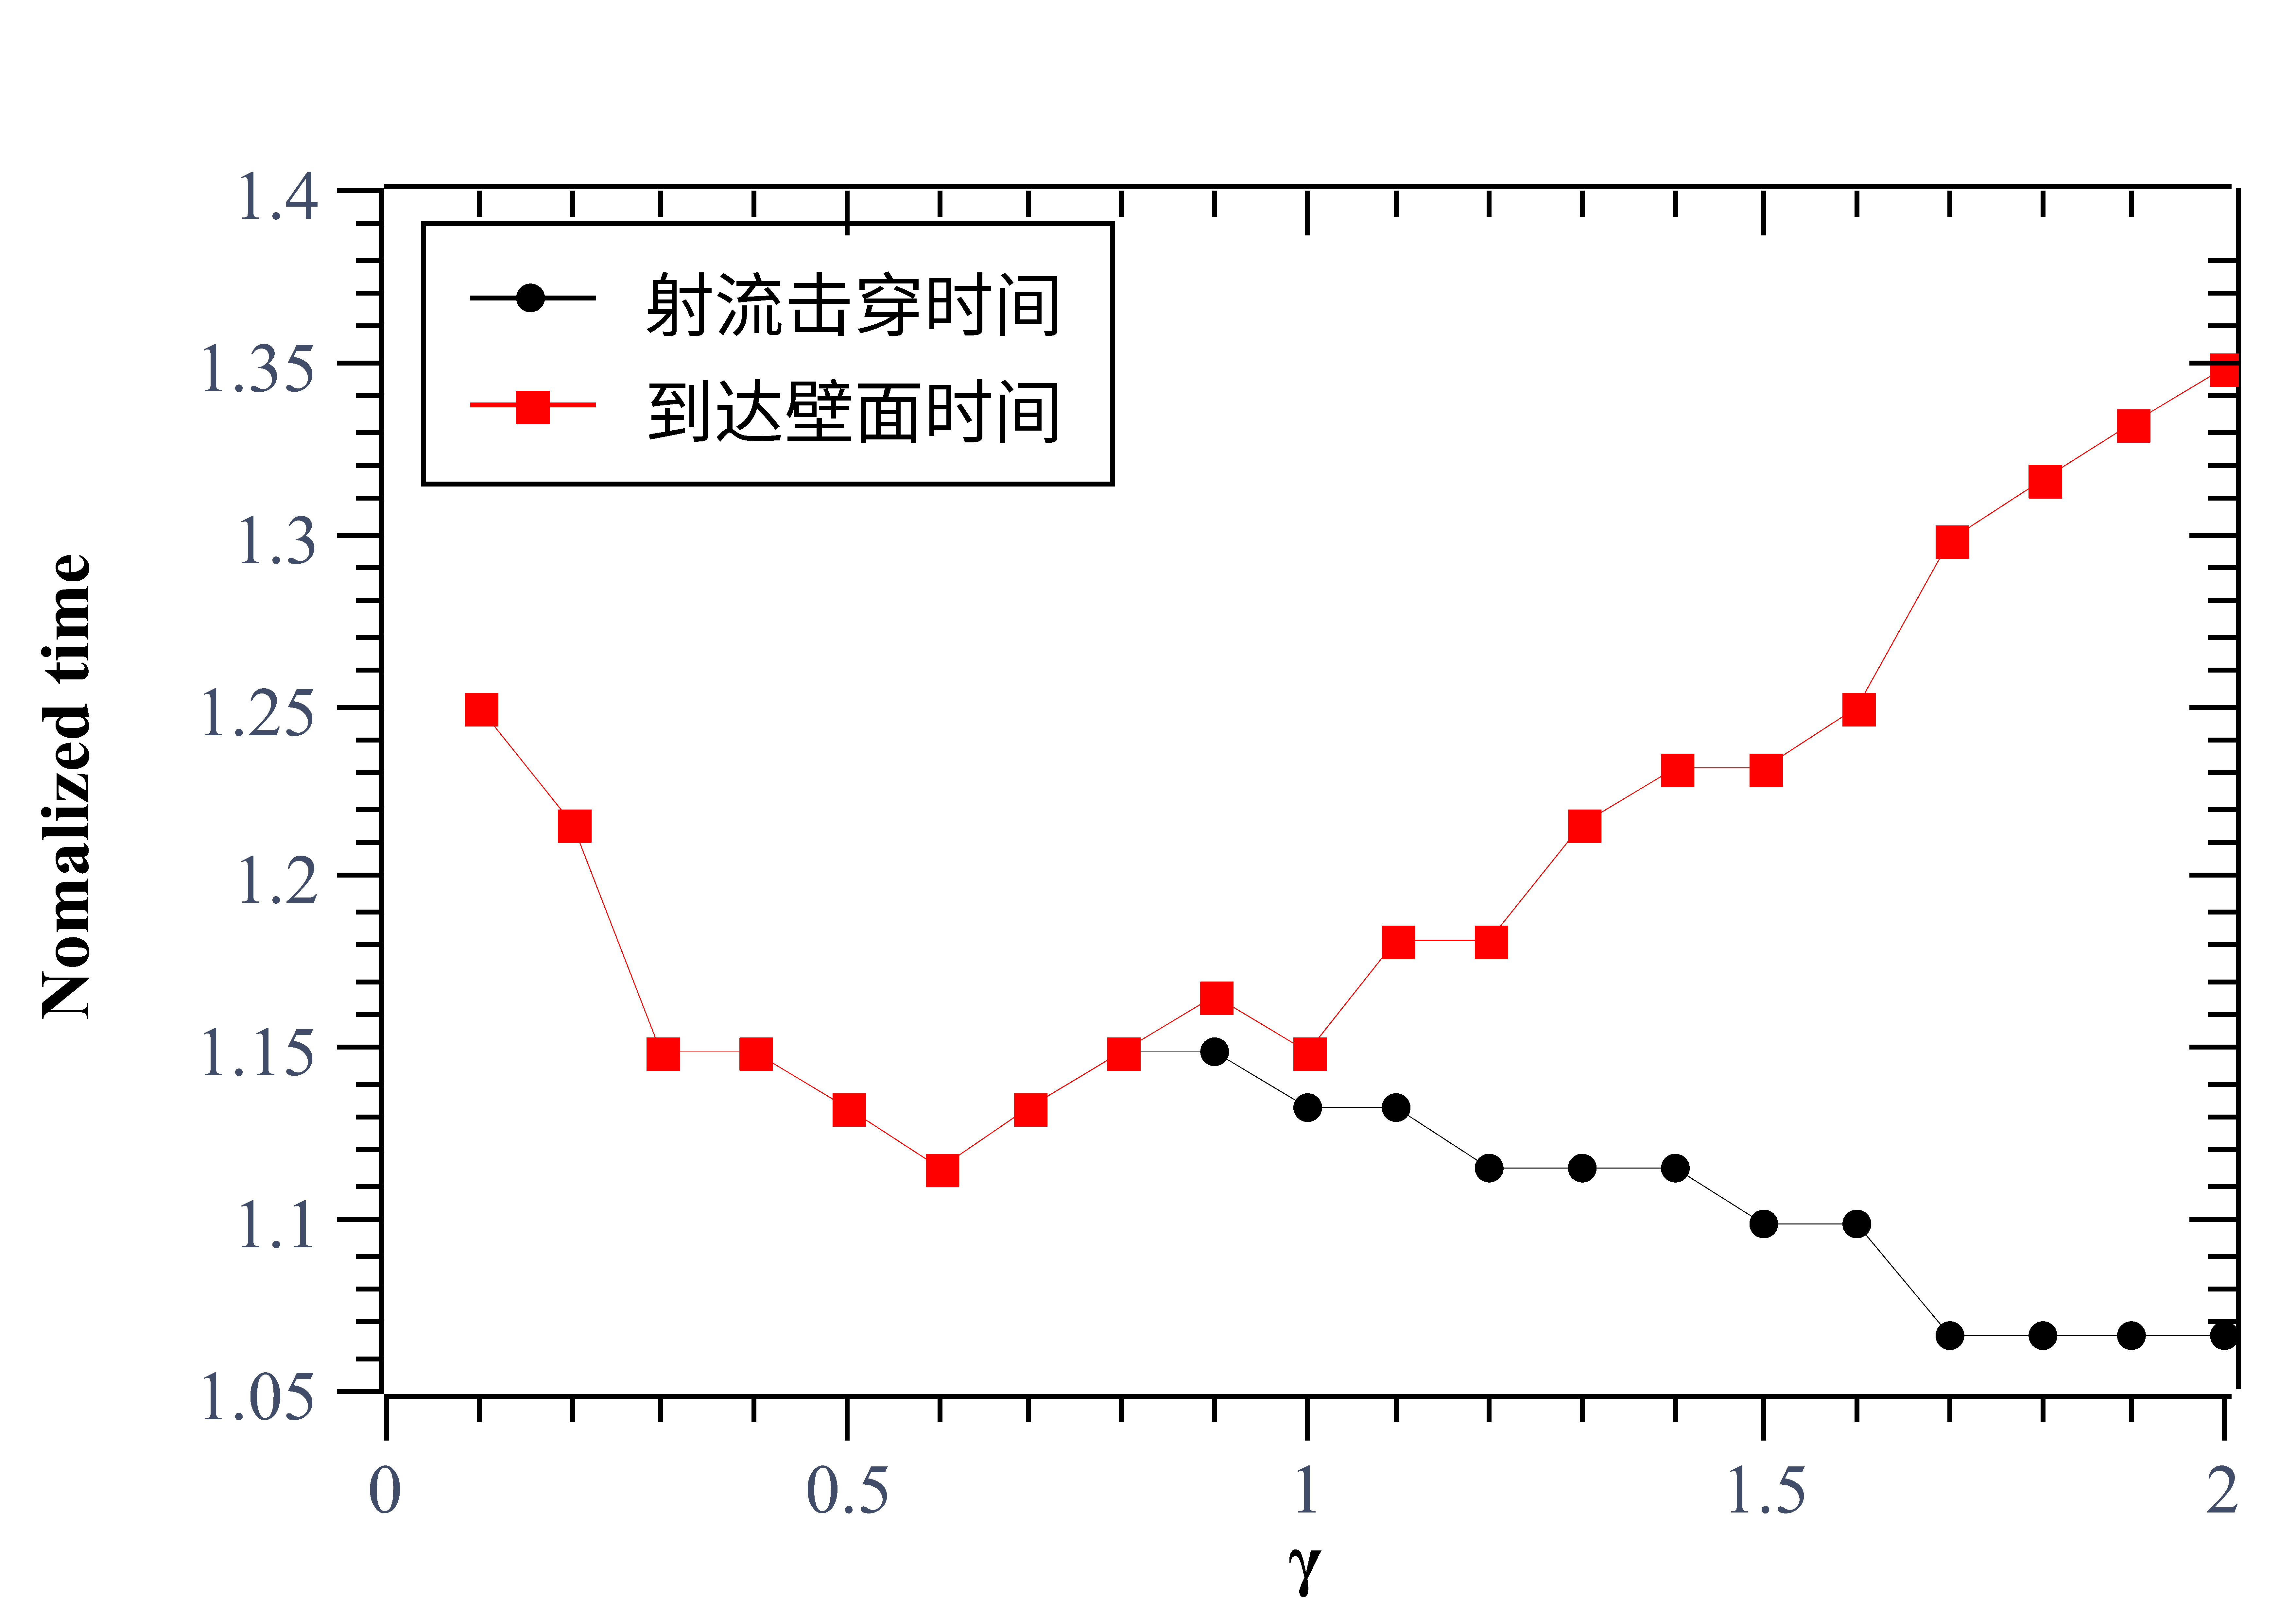
\includegraphics[width=0.9\linewidth]{img/solidtime.eps.pdf}
    \caption{空泡距固体界面不同相对距离情形下的射流击穿空泡时间和射流到达固体壁面的时间}
    \label{fig3.jettime}
\end{figure}

在以上三种情况中,都产生了各自特殊情况的射流。
图\ref{fig3.jettime}显示了空泡距固体界面不同相对距离情形下的射流击穿空泡的归一化时间和射流到达固体壁面的归一化时间。对大相对距离的情况,也就是$\gamma>1.7$时,射流击穿的归一化时间相当接近1.0,也就是射流击穿时间和自由单空泡的溃灭时间接近。也可以理解成,在这种情况下,空泡的射流击穿是在空泡的溃灭末期形成的,即空泡溃灭和空泡射流几乎同时。可以认为,$\gamma$越大这种同时性会越來越好。这与\ref{chapter1.2.2.2}中使用$\zeta$预言的结果一致。在$\gamma>0.7$时,空泡击穿的时间是递减的,也就是越脱离壁面的影响,空泡的击穿时间越接近自由空泡。而空泡到达壁面的时间是递增的,这与空泡离壁面位置越远到达壁面的时间越长的逻辑是一致的。$0.3\leq \gamma\leq0.8$范围内,空泡的膨胀贴近壁面,射流击穿空泡自身和到达壁面的时间几乎一致。而$\gamma\leq0.2$时,空泡表现出半球型膨胀和收缩,其空泡的体积等效半径与其他空泡类似,但因半球型而形成较大的上下空泡面距离,其形成的针状射流,时间较晚但速度较快。


\section{本章小结}


本章主要探讨了基于可压缩多相流模型的空泡在水-气、水-油、水-固界面附近的脉动情况。针对空泡距离不同界面不同位置做了空泡动力学分析和射流模式的分析。
在水气界面形成三种不同的相互作用机制:爆破型、皇冠射流型、和凸起型。
在水油界面则分成了断裂式溃灭和射流式溃灭。而其中断裂式溃灭又可以细分为断裂接触式和断裂射流式。
在水固界面也因三种空泡的脉动形式而形成多种射流机制:常规射流溃灭,和针状射流溃灭。常规射流又可以细分为空泡接触壁面和不接触壁面两种机制。

文中对空泡动力学和形态学进行了详细的解释,并分析了针对空泡与界面的距离对空泡与界面相互作用的规律性现象。

本模型也可应用于计算更多种不同界面形状和不同物性的空泡脉动。



